\documentclass[a4paper]{article}
\usepackage[a4paper,
top=1in, 
bottom=1in, 
left=1in, 
right=1in
]{geometry}
\usepackage{verbatim}
\usepackage[backend=biber,
style=authoryear,
bibencoding=utf8]{biblatex}
\usepackage{graphicx}
\usepackage{subcaption}
\usepackage{pythonhighlight}
\usepackage{xcolor}
\usepackage{tcolorbox}
\usepackage{xurl}
\usepackage{parskip}
\usepackage{titlesec}
\usepackage{longtable}
\usepackage{booktabs}
\usepackage{amsmath}

\setcounter{secnumdepth}{4}

\titleformat{\paragraph}
{\normalfont\normalsize\bfseries}{\theparagraph}{1em}{}
\titlespacing*{\paragraph}
{0pt}{3.25ex plus 1ex minus .2ex}{1.5ex plus .2ex}

\addbibresource{sources.bib}
\begin{document}

\includegraphics[width=\linewidth]{./logo.jpg}
\subsection*{Interuniversity Institute of Bioinformatics in Brussels}
\vfill
\section*{Large scale comparison between the biophysical landscape of cytoplasmic and periplasmic proteins with focus on the effect of signal peptides in Gram-negative Bacteria}

M\'emoire pr\'esent\'e en vue de l'obtention du dipl\^ome de Master en Bioinformatique et Mod\'elisation

\vfill
\subsection*{Jan Van den Schilden}
\subsection*{Promoter: Prof. Dr. Wim Vranken}
\subsection*{IB2}
\paragraph*{Academic year: 2019-2020}
\thispagestyle{empty}
\newpage

\tableofcontents
\newpage

\section{Introduction}
	% Part about UniProtKb
With protein and nucleotide sequencing getting cheaper every year, 
large-scale sequencing efforts are increasing the coverage of complete proteomes.
The amount of protein sequences in UniProtKB has been growing exponentially.
As on the moment this paragraph was written, 
UniprotKB contained a total of 181,252,700 protein sequences. 
562,253 were reviewed by expert curators and part of the UniProtKB/Swiss-Prot database.
180,690,447 unreviewed sequences are part of the UniprotKB/TrEMBL database. 
That means that experimental information about functionality or biophysical features is only available for about 0.3 percent of the proteins.
For 99.7 percent, only the protein sequence is known.
% Relation between protein function and primary sequence
Local and distant interactions along this the structure guide the folding process,
thereby determining structure , dynamics and function.
Essentially, all of the biophysical features are encoded within the primary sequence.
However, predicting and extracting these features, given only the protein sequence, has proven to be a challenging task,
and still a topic of ongoing research.

% More specific about dynamics
Traditionally, protein function was thought to be a direct result of protein structure,
But in recent years it has become clear that the structure provides only part of the picture.
Other biophysical features, such as the propensity toward dynamics, disorder, and early folding also seem to play a fundamental role for protein functionality.
A new generation of machine learning based predictors that only need a single protein sequence as input
are being developed at the Bio2Byte research lab at the Interuniversity Institute of Bioinformatics in Brussels.
These predictors are trained on in-solution characteristics that highlight the importance of local interactions.
Two such predictors are Dynamine, which predicts backbone an sidechain dynamics,
and EFoldMine, which predicts how likely amino acids are involved in early folding events.
Not only can these predictors predict biophysical features without relying on prior structural knowledge,
the predictions are also very fast,
making them scalable for computational high-throughput methods.

% Protein localization and signal peptides
Cells are organised into different subcellular compartments including
the cytoplasm, the periplasm, the cell wall, and the nucleosome.
Signal peptides are short polypeptides at the N-terminal end of proteins that act as zip-code within the cell,
providing information to the cell how to sort the proteome over the different compartments.
These peptides typically have a length between 25 and 30 residues.
In general, signal peptides display low sequence similarity,
but there is a strong conservation of biophysical properties.
While signal peptides play an important role in protein translocation,
they are on themselves insufficient to guarantee this process.
A study (\cite{orfanoudaki2017}) has shown that cytoplasmic proteins can be distinguished from the secreted with an accuracy up to 95 percent using only features present in the mature domain.
One prominent difference seems to be that secreted proteins delay the folding process 
and display an increased flexibility and dynamics.
The reason for this difference, and what biophysical effect signal peptides have on these characteristics remains unclear.

% What is unknown and what was researched
In this master thesis,
the biophysical features of cytoplasmic and periplasmic proteins were compared on an extensive Gram-negative Bacteria protein dataset.
In addition, the effect of signal peptides on these features was examined.
The dataset was extracted from the public database UniProtKB by making use of their annotation system.
Biophysical predictions were acquired with state of the art machine learning based predictors that require only a single protein sequence as input,
making this method applicable for the full protein sequence space.


\newpage

\section{Literature review}
%\input{0.protein_introduction/0.protein_introduction}
	\subsection{Central dogma of molecular biology}
		The central dogma of molecular biology (Fig. \ref{fig:central_dogma}) describes the flow of information from DNA (deoxyribonucleic acid), 
through RNA (ribonucleic acid) into proteins. 
During the transcription process,
DNA is duplicated into a complementary RNA strand, 
which acts as messenger to deliver the information to the ribosome. 
Ribosomes use the code embedded in the messenger RNA (mRNA) to construct 
a protein in a process called translation (\cite{crick1970}).

DNA is a linear polymer with a fixed backbone from which can extend 4 different bases: 
adenine (A),
cytosine (C), 
guanine (G),
and thymine (T). 
These bases combine into specific Watson-Crick base pairs,
held together by hydrogen bonds. 
This way, two single strands of DNA can combine into a double helix.
Each strand contains all information to form the other, 
providing a template for the DNA replication mechanism. 
These features combined with its robust nature make DNA the ideal candidate for storage
and heredity of information (\cite{berg2015}).

During transcription, 
the same Watson-Crick base pairing rules are used to copy the information to mRNA. 
The only difference being that the base thymine is replaced by an uracil base. 
The protein RNA polymerase synthesises a complementary strand of mRNA by reading the sense thread of dsDNA. 
The mRNA is transported through the cytoplasm to the ribosomes, 
which can be seen as the protein factories of the cell. 
Ribosomes read the mRNA template three bases at a time, also known as codons. 
Each codon is translated into a specific amino acid.
There are 64 different codons, yet only 20 distinct amino acids. 
This means that multiple codons encode the same amino acid. 
Codon for codon, the mRNA is translated into a linear polymer of amino acids.

~\begin{figure}[h!]
	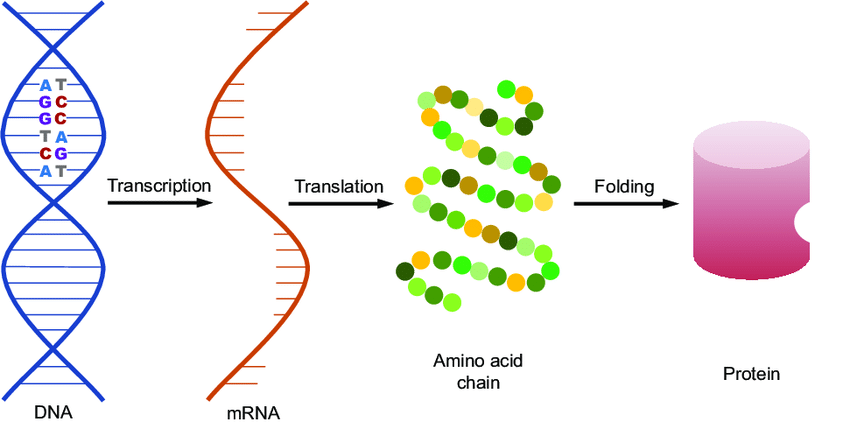
\includegraphics[width=\linewidth]{./literature_review/central_dogma/img/central_dogma.png}
	\caption{
	\textbf{Central dogma of molecular biology.}
	It describes the flow of molecular information, 
	starting from DNA, 
	through RNA, 
	and ending as a amino acid sequence. 
	Subsequently, this sequence folds into a functional protein.
	The transition from DNA to RNA is called transcription, 
	the transition from RNA to a protein is called translation
	(from \cite{cichonska2018}).	
	}
	\label{fig:central_dogma}
~\end{figure}

	\subsection{Proteins}
		Proteins fulfil the fundamental processes of life. 
Proteins consist of amino acids,
the building blocks that link together into a linear sequence, 
as beads of a pearl necklace.
This linear sequence is called the primary structure. 
Local and distant interactions between amino acids in the sequence will determine the fold and biophysical properties, 
and thus the function of the protein (Fig. \ref{fig:local_distant}).
To understand the difference between local and distant interactions,
we can visualise this  with the pearl necklace metaphor.
Imagine yourself unhooking the necklace and placing both ends far away from each other, forming a straight line.
Which beads are close to each other? 
Each bead is closest to its directly connected neighbours, 
a bit farther to the neighbours of the neighbours,
even further to their neighbours, and so on...
By placing the necklace as a straight line,
we have essentially reduced a three-dimensional necklace to a one-dimensional sequence.
When speaking about local interaction, 
it is meant as interactions between between beads that are close to each other in this one-dimensional space.
Proteins are not straight lines of amino acids however.
Just as a pearl necklace can make curves and fold upon itself, 
so do proteins.
This way beads that are very far away from each other in sequence,
can be close to each other in three-dimensional space and form interactions.
These are called distant interactions.
Each protein has its own unique local and distant interactions.
This way, 
they fold into different shapes and can so specialise for specific tasks.

~\begin{figure}[h!]
	\centering
	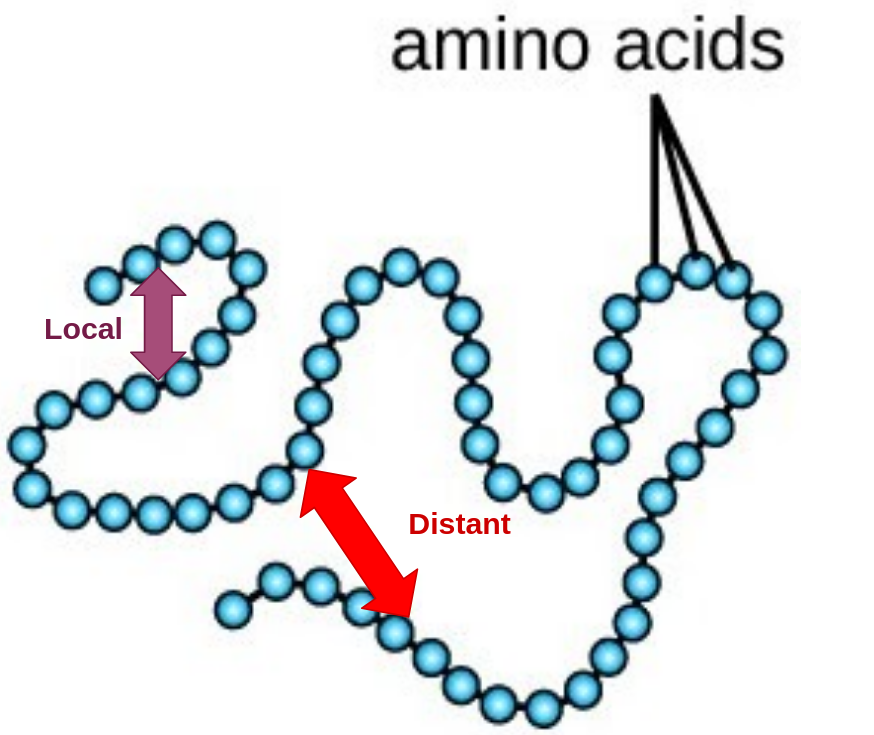
\includegraphics[width=0.6\linewidth]{./literature_review/proteins/img/local_distant.png}
	\caption{
		\textbf{Local and Distant interactions along the protein sequence}
		(adapted from https://tinyurl.com/y7aoehrt).
	}
	\label{fig:local_distant}
~\end{figure}

		\subsubsection{Amino acids}
			There are 20 different amino acids to act as building blocks for proteins (Fig. \ref{fig:amino_acids}).
This alphabet displays diverse structural and chemical properties, 
giving proteins the ability to assume many functional roles.
Each amino acid consist of a central $\alpha$-carbon,
which is linked to four different groups:
an amino group,
a carboxylic acid group,
a hydrogen atom,
and one of the 20 possible sidechains.
A wide range of functional groups can be displayed on the sidechain,
including alcohols,
a thiol,
a thioether,
carboxylic acids,
and various basic groups.
Because these 20 unique amino acids,
each with their own physico-chemical properties,
can be ordered in numerous ways in a protein sequence, 
there is broad spectrum of protein functionality
(\cite{berg2015}).

~\begin{figure}[h!]
	~\begin{subfigure}[b]{0.70\linewidth}
		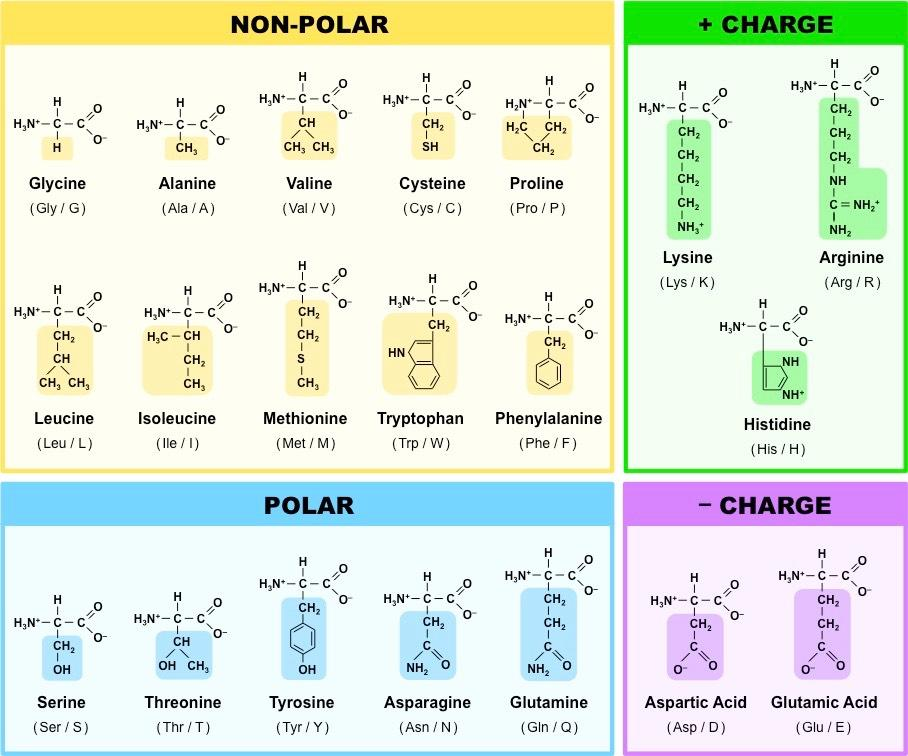
\includegraphics[width=\linewidth]{./literature_review/proteins/amino_acids/img/classification.jpg}
		\caption{\textbf{Classification}}
	~\end{subfigure}
	~\begin{subfigure}[b]{0.25\linewidth}
		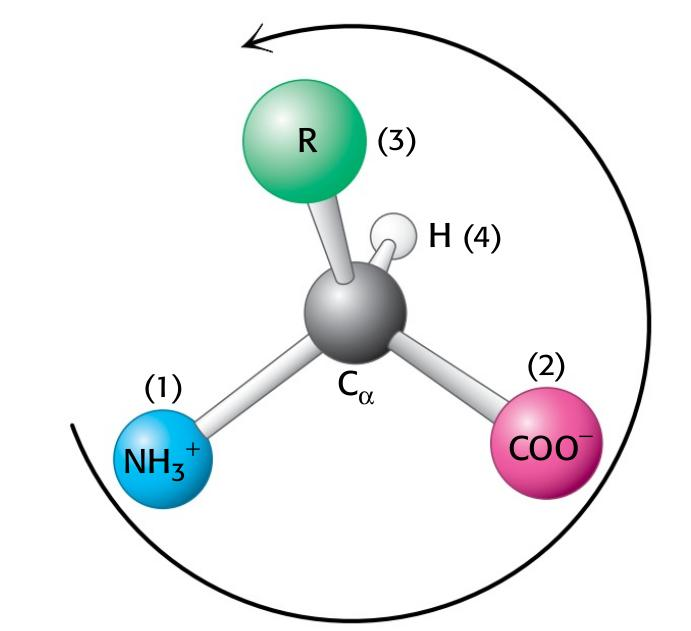
\includegraphics[width=\linewidth]{./literature_review/proteins/amino_acids/img/structure.jpg}
		\caption{\textbf{Structure}}
	~\end{subfigure}
	\caption{
		\textbf{Amino acids. a.}
	Amino acid classification by general chemical properties. 
	Each amino acid is depicted with its chemical structure, name, three-letter and one-letter code. 
	The sidechains are highlighted by a coloured frame 
	(from ib.bioninja.com.au).
		\textbf{b.}
	The general structure of an amino acid. 
	A central alpha-carbon is connected to 
	an amino group (blue),
	a carboxylic acid group (pink),
	an hydrogen atom (white),
	and a one of the 20 sidechains (green).
	(from \cite{berg2015}).
	}
	\label{fig:amino_acids}
~\end{figure}

		\subsubsection{Primary structure}
			The primary structure of a protein can be described as a linear sequence of amino acids, also called residues.
They are connected to each other by peptide bonds (Fig. \ref{fig:primary_structure}).
These amide bonds link the $\alpha$-carboxyl group of one amino acid to the amino group of the next.
A polypeptide chain has directionality, 
by convention it start with the amino group and ends with the carboxyl group. 
In the sequence YGGLHAV, Tyrosine (TYR, Y) is the amino-terminal (N-terminal) residue and Valine (VAL, V) the carboxyl-terminal (C-terminal) residue.
The reverse sequence VAHLGGY will have other chemical properties and display other dynamical and conformational behaviour.
Therefore it is considered a different peptide.
The $\alpha$-carbon ($C_{\alpha}$) plus the amino group (NH) and carboxylic acid group (CO) that are connected to it are the same for every residue.
Therefore, a repeating pattern (...-NH-$C_{\alpha}$-CO-NH-...) is observed throughout the sequence.
This constant pattern is called the backbone or mainchain of the protein.
Each residue has also a variable sidechain.
As opposed to DNA,
the backbone of proteins is uncharged.
Therefore, amino acids polymers can form tightly packed globular structures
(\cite{berg2015}).

~\begin{figure}[h!]
	\centering
	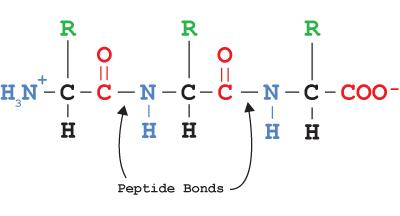
\includegraphics[height=0.25\textheight]{./literature_review/proteins/primary_structure/img/primary_structure.jpg}
	\caption{
		\textbf{The primary structure of a small peptide with three amino acids.}
	(from cbm.msoe.edu).
	}
	\label{fig:primary_structure}
~\end{figure}

		\subsubsection{Secondary structure}
			% torsion angles
The backbone of a polypeptide chain is flexible and changes shape by rotating around its bonds.
There are three different angles of rotation for every residue in a protein,
also called torsion angles (Fig. \ref{fig:torsion_angles}).
The rotation angle around the peptide bond, 
connecting the amino group with carboxylic acid group,
is called $\omega$.
The torsion angles around the bond that connect the amino group with $\alpha$-carbon is $\phi$,
and $\psi$ is the angle around the bond that connects the $\alpha$-carbon with the carboxylic acid group.

A protein in disordered state is highly dynamical and can rotate relatively freely around its torsion angles.
In folding the proteins fixes most of these torsion angles, 
thereby losing entropy.
For folding to be spontaneous, 
the protein needs to compensate for this loss of entropy with a negative change in enthalpy.
This is done by forming molecular interactions 
(e.g. hydrogen bonds, Van Der Waals interactions, electrostatic interactions, etc).
Should all the torsion angles be able to rotate the full 360 degrees,
the entropic loss would be to great to overcome
and the protein would never fold.
This is only a simplified explanation,
the reality is more complex as also the entropy and enthalpy of the surrounding environment,
especially the water molecules, have to be taken in to account.

Torsion angles are restricted however.
The $\omega$ angle describes the rotation around the peptide bond.
Because peptide bonds have a partial double-bond character, 
only two conformations are energetically allowed: 
cis conformation (0 degrees) (Fig. \ref{fig:cis}),
and trans conformation (180 degrees) (Fig. \ref{fig:trans}).
For sterical reasons,
the trans conformation is more frequently observed.
For similar sterical reasons,
not all $\phi$ and $\psi$ angle combinations are  physically possible.
Allowed combination can be visualised on a Ramachandran plot
(\cite{berg2015}).
Within these allowed Ramachandran plot regions,
regular repeating arrangements can arise to form secondary structures,
The most common being $\alpha$-helices and $\beta$-strands.

~\begin{figure}[h!]
	~\begin{subfigure}[b]{0.32\linewidth}
		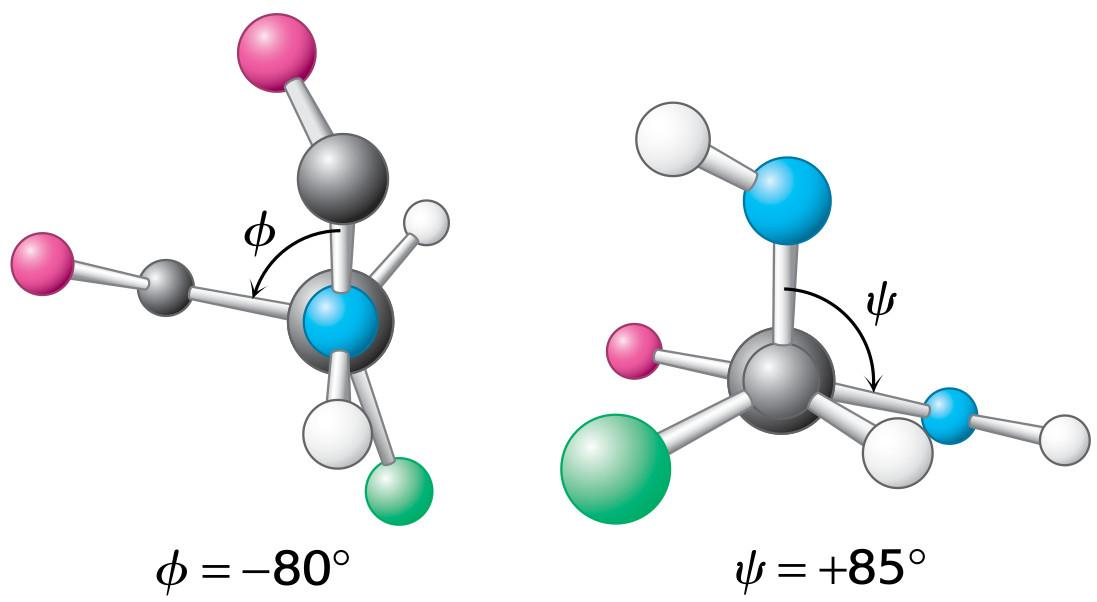
\includegraphics[width=\linewidth]{./literature_review/proteins/secundary_structure/img/torsion_angles.jpg}
		\caption{\textbf{Torsion angles}}
		\label{fig:torsion_angles}
	~\end{subfigure}
	~\begin{subfigure}[b]{0.32\linewidth}
		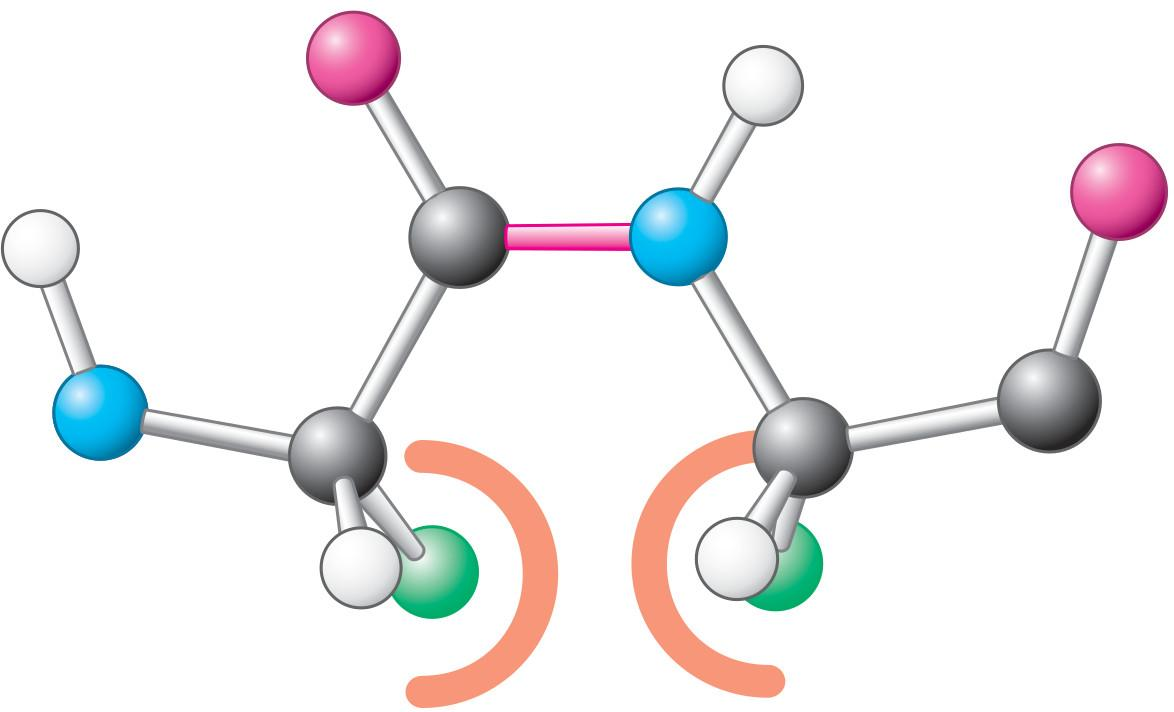
\includegraphics[width=\linewidth]{./literature_review/proteins/secundary_structure/img/cis.jpg}
		\caption{\textbf{Cis}}
		\label{fig:cis}
	~\end{subfigure}
	~\begin{subfigure}[b]{0.32\linewidth}
		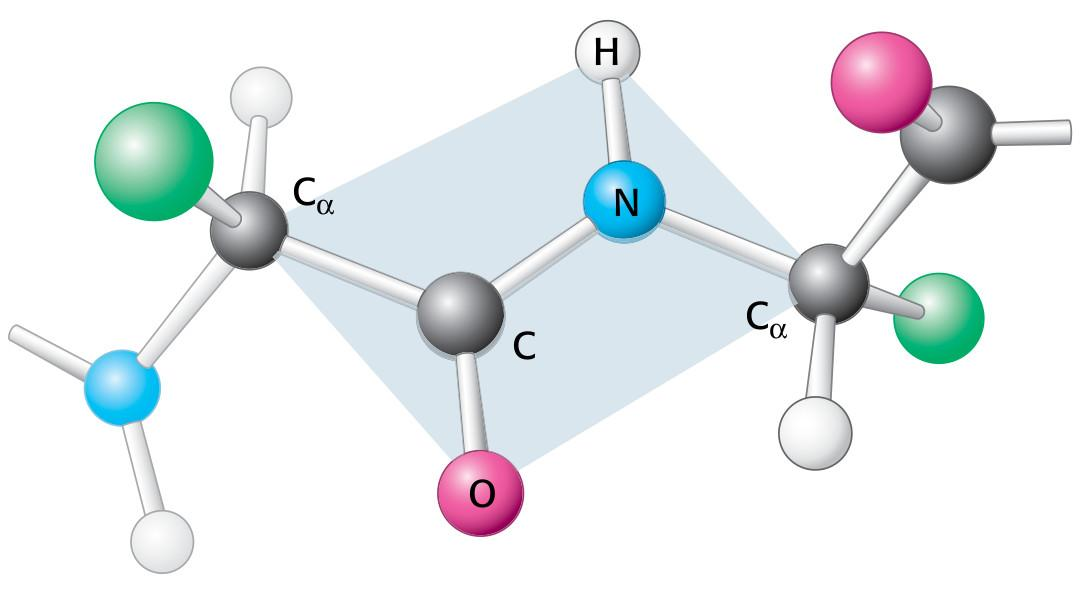
\includegraphics[width=\linewidth]{./literature_review/proteins/secundary_structure/img/trans_planar.jpg}
		\caption{\textbf{Planarity of peptide bond, trans}}
		\label{fig:trans}
	~\end{subfigure}
	\caption{
		\textbf{Peptide bond and torsion angles.}
	Green:R-group,
	Black:Carbon,
	Purple:Oxygen, 
	Blue:Nitrogen,
	White:Hydrogen
		\textbf{a.}
	The partial double bond-character character of peptide bonds ensures that 6 atoms lie in the same plane for every pair of amino acids. 
	The peptide bond is shown in trans configuration.
		\textbf{b.}
	In cis configuration, sidechains will experience energetically unfavorable steric clashes.
		\textbf{c.}
	Torsion angles.
	(From \cite{berg2015}).
	}
~\end{figure}

			\paragraph{Alpha helix}
				~\begin{comment}
Fig. \ref{fig:local_helix}) shows that cytoplasmic proteins have a higher propensity to form a helix at the beginning and near residue position 25 (as shown by the bump in the blue curve).
More C-terminal position do not show this preference as is depicted by the relatively even curve.
Mature periplasmic domains on the other hand seem to have a lower propensity toward helix formation as is observed starting from position 0 going to position 75.
The signal peptide itself displays a high tendency towards this secondary structure however, 
and this effect seems to be propagated to the N-terminal part of the periplasmic proteins.

Why cytoplasmic proteins have an increased tendency to form helices at near position 0 and 25,
while this is decreased in the mature domains of the periplasm remains unclear.
These same general regions seem to have a relative high propensity toward early folding both in cytoplasmic and periplasmic proteins and (Fig. \ref{fig:local_earlyfolding),
though in periplasmic proteins they are shifted toward the C-terminal end.
This could suggest that these regions play an important role in the folding process,
decreasing the propensity toward helix formation possible has a delaying effect.
~\end{comment}


			\paragraph{Beta sheet}
				A $\beta$-strand is a polypeptide chain that is almost fully extended, 
with the sidechains of neighbouring residues directed in opposite orientations (Fig. \ref{fig:sheet}). 
Folding the chain back and forth brings $\beta$-strands next to each other, 
which allows them to undergo hydrogen bonding and form a $\beta$-sheet.
Adjacent residues along the strand point in opposite directions and the distance between them is 3.5 Å. 
Neighbouring strands either run in the same or opposite directions. 
This forms a antiparallel, parallel, or mixed $\beta$-sheet
In antiparallel arrangement (middle and bottom strand),
the NH group and CO group of an amino acid are hydrogen bonded with a partner amino acid in the neighbouring strand.
The parallel arrangement is more complicated.
Each amino acid of one strand forms hydrogen bonds with two amino acids of the adjacent strand. 
Finally, in the mixed sheet parallel and antiparallel neighbouring strands are mixed in one sheet
(\cite{berg2015}).

~\begin{figure}[h!]
	\centering
	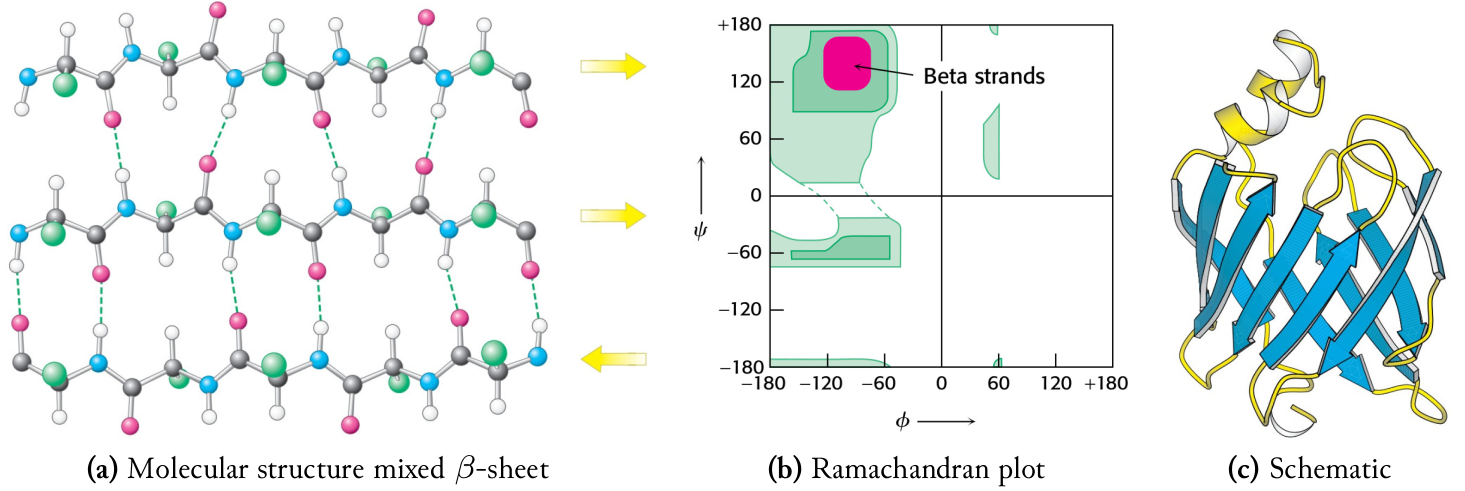
\includegraphics[width=\linewidth]{./literature_review/proteins/secundary_structure/sheet/img/sheet.png}
	\caption{
		\textbf{$\beta$-sheet secondary structure. a.}
	Molecular structure of a mixed $\beta$-sheet. 
	Adjacent residues along the strand point in opposite directions and the distance between them is 3.5 Angstron. 
	In antiparallel arrangement (middle and bottom strand),
	the NH group and CO group of an amino acid are hydrogen bonded with a partner amino acid in the neighbouring strand.
	The parallel arrangement is more complicated (top strand and middle strand). 
	Each amino acid of one strand forms hydrogen bonds with two amino acids of the adjacent strand. 
	Green:R-group, 
	Black:Carbon, 
	Purple:Oxygen, 
	Blue:Nitrogen,
	White:Hydrogen, 
		\textbf{b.}
	Situation of $\psi$ and $\phi$ angles of the $\beta$-strand on the Ramachandran plot.
		\textbf{c.}
	Schematic representation of a protein rich in $\beta$-sheets.
	}
	\label{fig:sheet}
~\end{figure}

		\subsubsection{Tertiary and quaternary structure}
			Whereas secondary structures are mainly determined by local interactions, 
so are tertiary structures in addition influenced by distant interactions. 
Hydrophobic interactions are the main driving force in determining the tertiary structure, 
but hydrogen bonds, 
disulfide bonds 
and ionic bonds 
play an important role as well 
(\cite{madigan2015}). 
It is thermodynamically more stable to cluster hydrophobic groups together than expose them to the aqueous environment. 
Therefore, a protein folds in such a way that nonpolar sidechains are buried inside the core 
and polar sidechains reside on the surface.
Multiple macromolecules can form a complex with the tertiary structure, this is called the quaternary structure.
Proteins are versatile in that the tendency to form specific local and distant interactions,
which secondary structures will be formed, 
and even the final fold, 
are all encoded within the primary structure (Fig. \ref{fig:topology})
(\cite{berg2015}).


~\begin{figure}[h!]
	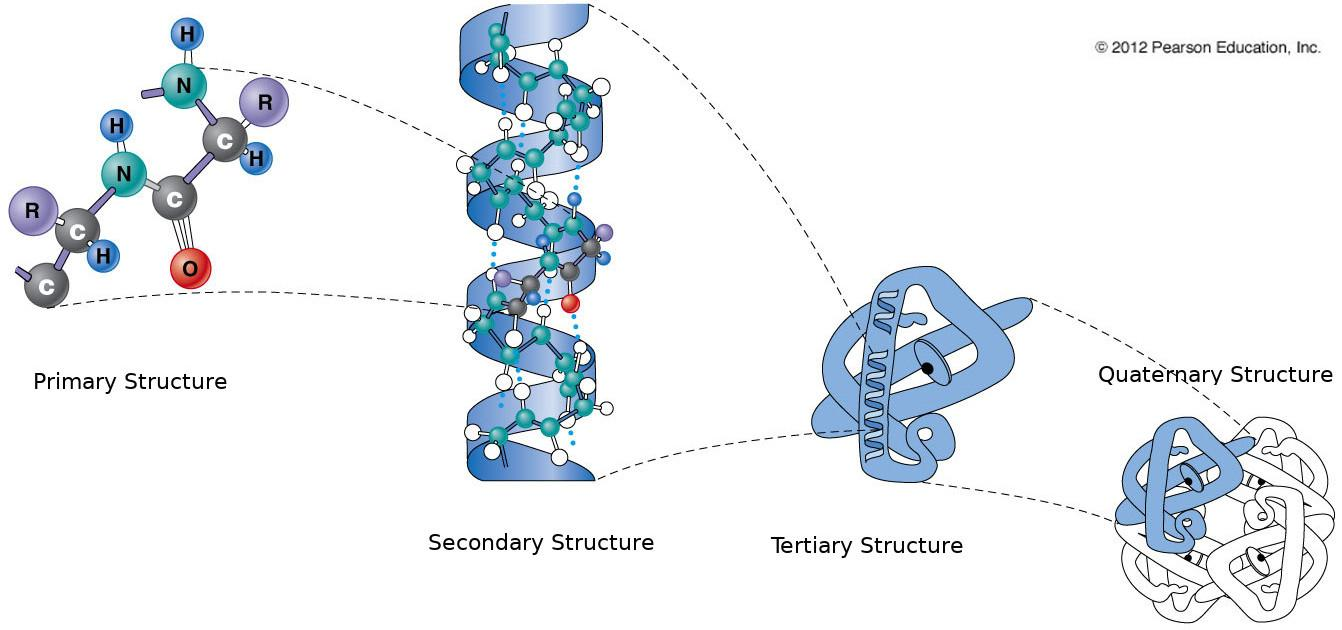
\includegraphics[width=\linewidth]{./literature_review/proteins/tertiary_quaternary/img/topology.jpg}
	\caption{\textbf{Different levels of protein topology.}}
	\label{fig:topology}
~\end{figure}
	
		\subsubsection{Dynamics}
			The structure of a protein is important for its final function,
however it is not the full story.
Dynamics in the backbone and sidechain are necessary for protein functionality,
but also guide the protein folding process.
As with structure,
dynamical preferences are encoded within the primary sequence.


			The importance of dynamics in proteins is highlighted in intrinsically disordered proteins (IDP).
In contrast with more traditionally studied proteins,
they do not need to adopt a defined three-dimensional fold to achieve their function.
Instead, they remain in a disordered, more coil-like state,
where no particular well-defined conformation is adopted by the protein.
In fact, for many IDP's there function seems to depend on the protein remaining in this disordered state most of the time,
only folding upon interaction
(\cite{van2014}).

Fully structured proteins and IDP's are only two ends of a spectrum, 
with a lot of possibilities in between (Fig. \ref{fig:structure_disorder}).
In fact, many structured proteins have at least some intrinsically disordered regions (IDR's).
For example,
it is estimated that 44 percent of the human proteins contain a disordered region of 30 amino acids or more.
Initially, those regions were thought to be linkers between functional, structured regions, but remaining passive otherwise.
However, it has now been established that these regions participate in a variety of functions,
such as interacting with other domains and post translational modifications (PTM's).
Other functionalities include molecular recognition,
molecular assembly,
and entropic chains
(\cite{van2014}).

~\begin{figure}[h!]
	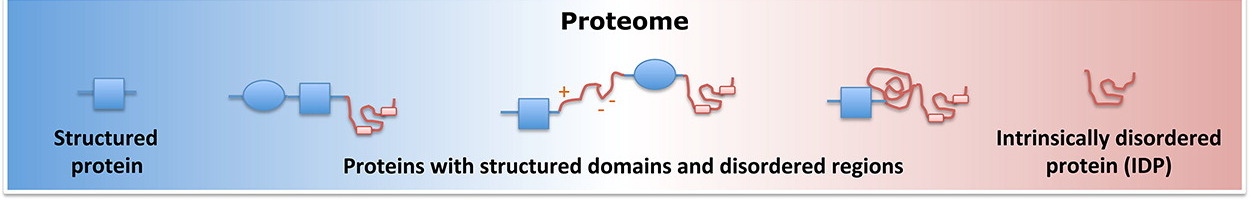
\includegraphics[width=\linewidth]{./literature_review/proteins/dynamics/img/protein_classes.jpeg}
	\caption{
	\textbf{Order and disorder in proteins.}
Proteins exist as a spectrum of dynamical possibilities,
ranging from fully structured and relatively rigid 
to fully disordered.
(adapted from \cite{van2014}).
}
	\label{fig:structure_disorder}
~\end{figure}

	\subsection{Protein feature prediction}
		Traditionally, 
protein function was tightly associated with structure,
but this is only part of the picture.
Many different biophysical features determine protein function:
structure,
hydrophobicity,
backbone and sidechain dynamics,
early folding propensity,
aggregation propensity,
solvent exposure,
and many more.
And essentially all are encoded within the primary sequence.
Extracting them remains challenging, but many efforts are being made,
as extracting biophysical features and to understand their relation to sequence space would greatly improve our understanding in proteins (Fig. \ref{fig:sequence_feature_relation}).
It would also help advance the field of protein design.
It is considered by some to have potential similar the to industrial revolution by the many application in 
medicine,
genetic circuit design,
bottom up nano technology,
and much more.


~\begin{figure}[h!]
	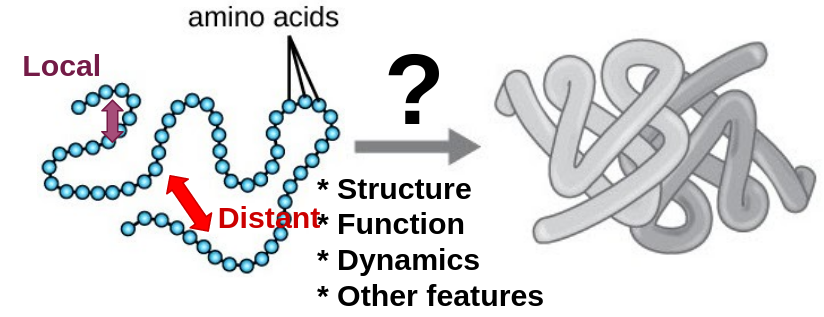
\includegraphics[width=\linewidth]{./literature_review/feature_prediction/biophysical_landscape/img/feature_prediction.png}
	\caption{\textbf{The protein sequence encodes its biophysical features.}
Local and distant interactions in protein sequence determine its biophysical properties,
but the mechanism are still a topic of active research.
}	
	\label{fig:sequence_feature_relation}
~\end{figure}


		\subsubsection{Sequence based predictors of biophysical features}
			While it is still not possible to predict the behaviour of the whole protein from sequence, 
there exist machine learning based predictors that can predict certain characteristics. 
A new generation of predictors, developed at the VUB, 
use in-solution characteristics of proteins and include information about intrinsically disordered regions, setting them apart om structure-based methods. 
The predictions are based on statistical information and highlight the importance of local interactions in a sequence between amino acids close to each other in the sequence, and the relative positions of different residues, 
e.g. a tyrosine could hypothetically increase the backbone dynamics when 3 amino acids apart from a valine, 
but reduce it when 7 amino acids apart. 
These predictions are very fast, which makes them scalable for computational high-throughput methods. 
DynaMine (\cite{cilia2013}) predicts the backbone dynamics of a protein. 
The predictor is trained on NMR data of proteins in solutions. 
Disordered regions are identified with similar accuracy as compared to the best other predictors, 
but without relying on structural information or prior disorder knowledge.
It even shows great potential in distinguishing between folded domains, molten globules, disordered linkers and pre-structured binding motifs of different sizes. 
Other DynaMine flavors, for sidechain dynamics and secondary structure propensities, 
were developed to create EFoldMine (\cite{raimondi2017}). 
This method predicts which amino acids are likely involved in early folding events, as detected by hydrogen deuterium exchange data from NMR pulsed labelling experiments. 
Predicted early folding residues are frequently those with a lot of interactions in the folded structure and they also display evolutionary covariation. 
Early folding events are likely defined by intrinsic local interactions and could have lasting effect in subsequent states. 

	\subsection{Subcellular localization of the proteome}
		\subsubsection{Protein localization}
			Cells are organised in different subcellular structures,
which is more complex in the Eukarya compared to the Bacteria and Archaea.
Different eukaryotic cellular structures include:
the nucleus,
plasma membrane,
cell wall,
different types of organelles,
and the endoplasmic reticulum.
By separating the cell in subcellular compartments, 
there can be a physical separation of different functions.
For example,
Mitochondria focus on the production of energy,
chloroplasts capture electromagnetic energy  by storing it into carbon based molecules,
and the nucleus contains the genetic information.
In addition, each compartment has its own local environment and conditions,
evolutionary tuned to the function it has to perform.
Animal and plant subcellular compartments are the most studied structures (Fig. \ref{fig:eukaryotic_cell_structure}).
While they both contain 
a nucleus, 
cytoplasm,
plasma membrane, 
endoplasmic reticulum,
and mitochondria,
there are some striking differences as well. 
The centrosome and lysosomes are unique organelles form animal cells. 
Plant cells on the other hand have a 
cell wall, 
a large central vacuole, 
chloroplasts and other specialized plastids
(\cite{boundless_biology_eukaryotic}).

~\begin{figure}[h!]
  \centering
  ~\begin{subfigure}[b]{0.45\linewidth}
    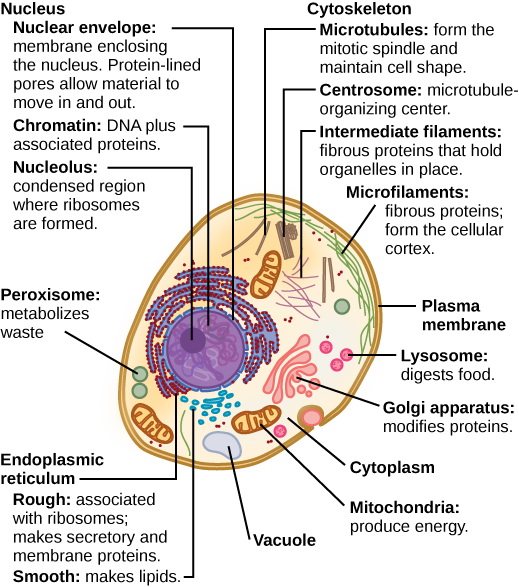
\includegraphics[width=\linewidth]
	{./literature_review/subcellular_location/protein_localization/img/animal_cell_structure.png}
  \caption{Animal cell}
  ~\end{subfigure}
\hfill
  ~\begin{subfigure}[b]{0.48\linewidth}
    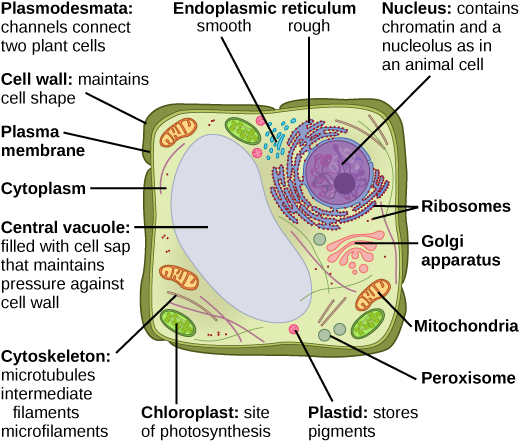
\includegraphics[width=\linewidth]
	{./literature_review/subcellular_location/protein_localization/img/plant_cell_structure.png}
  \caption{Plant cell}
  ~\end{subfigure}
  \caption{
\textbf{The eukaryotic cell structure.} 
Eukaryotic cells are subdivided in different subcellular compartments.
Shown are the animal and plant cell.
(from \cite{boundless_biology_eukaryotic}).
}
  \label{fig:eukaryotic_cell_structure}
~\end{figure}

The prokaryotic cell structure of Bacteria and Archaea is less complex than the eukaryotic structure.
Similarly, the plasmamembrane contains the cytoplasm.
Unlike eukaryotes, prokaryotic genetic DNA is not encapsulated by a nucleus,
but localised in a region called the nucleoid.
Prokaryotic cells are much smaller their eukaryotic counterparts,
and they lack organelles
(\cite{boundless_biology_prokaryotic}).
Bacteria can be divided into two major groups based on their Gram stain reaction
(Fig. \ref{fig:prokaryotic_cell_structure}).
Gram-negative cells have a cell wall that is made out of two layers:
a small peptidoglycan layer, 
and outer membrane containing a lipid bilayer and polysacharides.
The region between the inner and outer membrane is called the periplasm.
Gram-positive Bacteria have a thick mono-layer cell wall, mostly made out of peptidoglycan,
but no outer membrane
(\cite{madigan2015}).


~\begin{figure}[h!]
  \centering
  ~\begin{subfigure}[b]{\linewidth}
    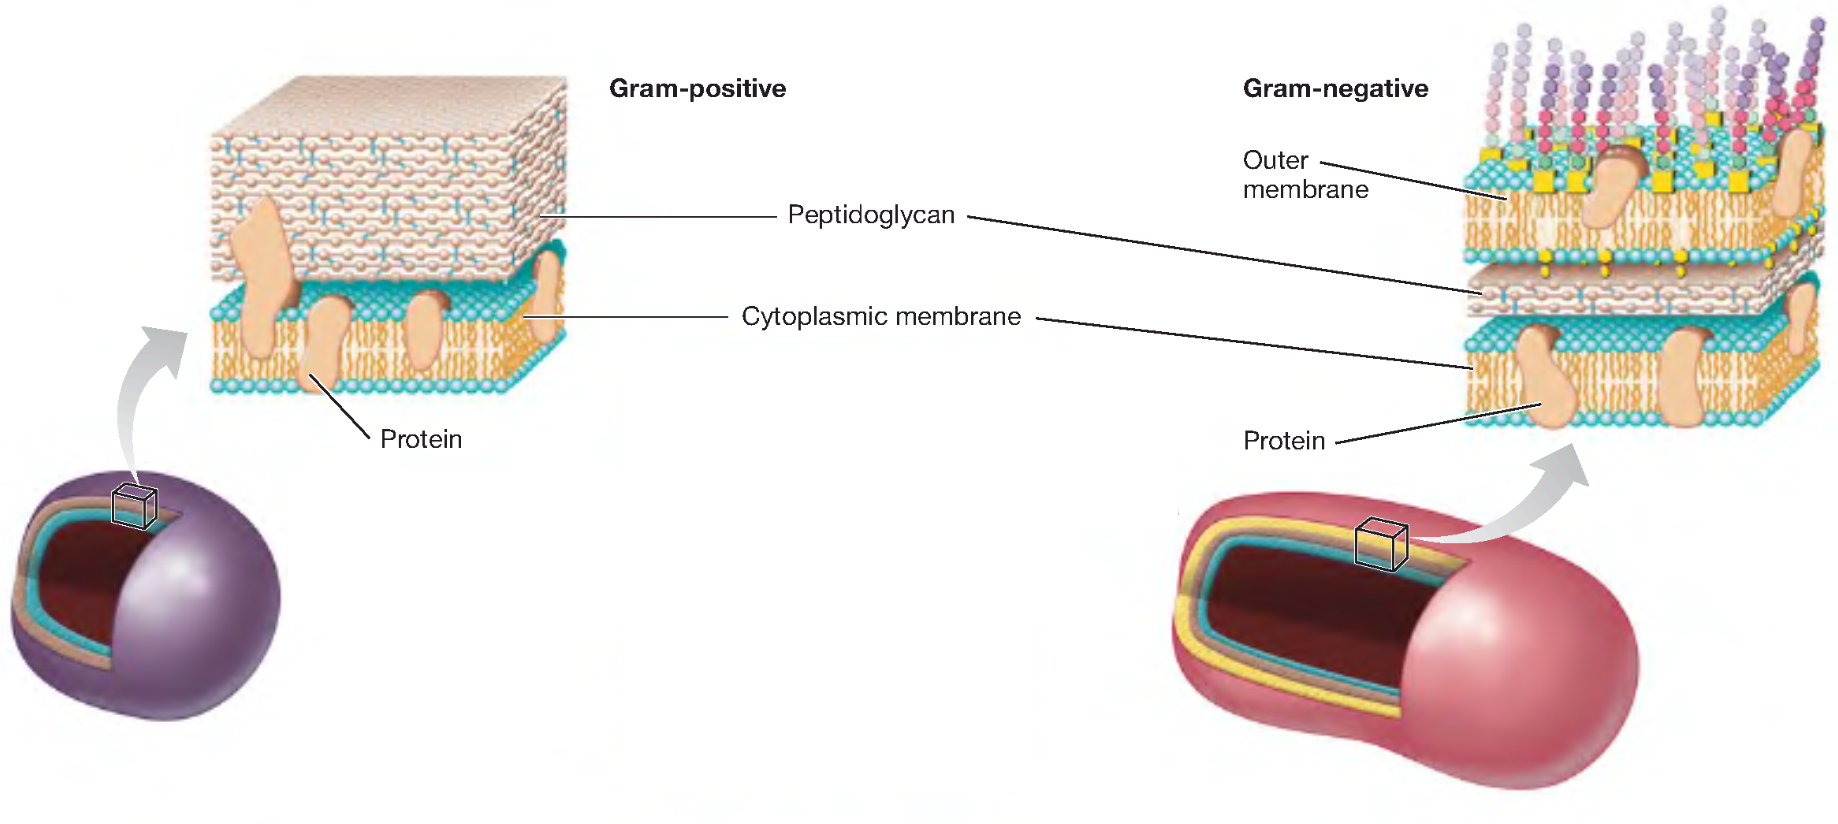
\includegraphics[width=\linewidth]
	{./literature_review/subcellular_location/protein_localization/img/gram_pos_vs_neg.png}
  ~\end{subfigure}
  \caption{
\textbf{The prokaryotic cell structure of gram positive and gram negative Bacteria.} 
(adapted from \cite{madigan2015}).
}
  \label{fig:prokaryotic_cell_structure}
~\end{figure}



		\subsubsection{proteome distribution}
			The proteome,
the collection of different proteins used by the cell, 
is distributed over the different cellular compartments.
Proteins are found on DNA,
near ribosomes,
on membranes,
through membranes,
or become excreted.
In many Bacteria,
up to and more than a third of the proteins exit the cytoplasm,
also called the exportome.
These proteins are either embedded in the inner membrane,
reside in the cell envelope,
or are fully released in the external environment. 
In vivo,
they fulfill a variety of function like 
signalling,
transport,
and membrane biogenesis and maintenance.
Unraveling what kind of function, interactions and dynamics proteins display on their way to and inside their final location
will help to improve our general biophysical understanding of proteins and their evolutionary connections (\cite{loos2019}).
More practically, it can help improve the efficiency of recombinant protein productions,
a tool used in pharmaceutical and industrial protein production (\cite{owji2018}).
For proteins to end up in the right location,
the cell has to overcome multiple challenges.
First it needs to be able to distinguish between those protein that stay in the cytoplasm and those that have to leave it.
As cells have no internal eyes, 
recognition needs to be achieved by physical contact between internal receptors and the target protein.
This is no easy task as the cytoplasm is very crowded (Fig. \ref{fig:crowding}).
Secondly, recognised proteins need to associate with or cross through the plasmamembrane. 
Proteins are big, bulky macromolecules that need special pathways to pass the membrane.
Additionally, exported proteins tend to delay their folding.
Protein trafficking if influenced by both extrinsic factors and intrinsic factors.
Extrinsic factors include 
the cellular environment of nascent proteins,
protein concentration,
proteostatic pathways,
and translocases.
Intrinsic factors on the other hand originate from the polypeptide itself, 
but are often poorly understood:
order / disordered regions,
3D fold and motifs,
nucleotide binding domains,
and signal peptides
(\cite{loos2019}).


~\begin{figure}[h!]
  \centering
  ~\begin{subfigure}[b]{0.45\linewidth}
    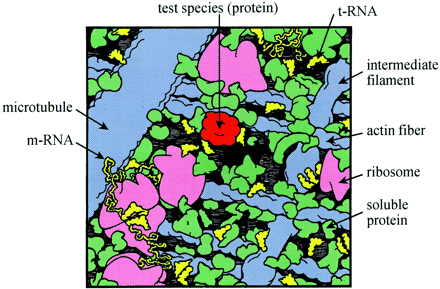
\includegraphics[width=\linewidth]
{./literature_review/subcellular_location/proteome_distribution/img/crowding_cartoon.png}
  \caption{Cartoon}
  ~\end{subfigure}
\hfill
  ~\begin{subfigure}[b]{0.48\linewidth}
    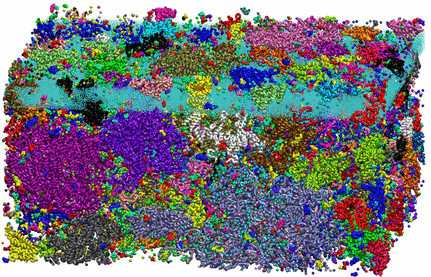
\includegraphics[width=\linewidth]
{./literature_review/subcellular_location/proteome_distribution/img/crowding_MD.png}
  \caption{Molecular dynamics simulation}
  ~\end{subfigure}
  \caption{
\textbf{Crowding in the cytoplasm.} 
\textbf{a.}
Cartoon representation of crowding in the cytoplasm at a magnification of 1,000,000.
Soluble proteins are shown in green,
RNA species in yellow,
cytoskeletal fiber in blue,
and ribosomes in pink
(from \cite{minton2001}).
\textbf{b.}
Molecular dynamics simulation of crowded cellular system.
The cytoplasm consists of proteins, RNA, metabolites, ions, and water
(from \cite{feig2017}).
}
  \label{fig:crowding}
~\end{figure}





		\subsubsection{Signal peptides}
			Signal peptides have been elaborately studied since they were first hypothesized by Blobel and Sabatini (\cite{blobel1971}).
They are short polypeptides at the N-terminal end of proteins, the part that is generated first by ribosomes,
and carry information for the protein target location or secretion.
They occur in all domains of life and have been of interest both industrial and scientific fields,
ranging from industrial recombinant protein production and biotherapeutics to immunization and laboratory techniques (\cite{owji2018}).
The gram positive model organism \textit{Bacillus subtilis} contains for about 50 percent of the extracellular proteins a typical signal peptide (\cite{humphery2006})
For the gram negative model organism \textit{Escherichia coli}, this is more than 90 percent (\cite{rusch2007}),
and also eukaryotes contain a significant amount of secretory proteins with signal peptide (\cite{kanapin2003}).
Even though multiple studies examined signal peptide function and structure,
some features remain to be elucidated.


			
			Signal peptides typically have a length between 25 and 30 residues
(\cite{von1990}),
but long signal peptides up to 140 residues are found in eukaryotes.
Longer signal peptides most often target organelles, 
where they remain stable after translocation, giving the protein additional functionality.
Evolutionary, signal peptides  display low sequence similarity,
but there is a strong conservation of biophysical properties
(\cite{paetzel2002}).
Three regions are distinguished 
(Fig.~\ref{fig:signal_peptide_structure}):
a positively charged N-terminal end,
a central hydrophobic patch,
and an hydrophilic C-terminal region that contains the conserved signal peptidase cleavage site
(\cite{orfanoudaki2017}).
The high degree of sequential variation of signal peptide composition is believed to be responsible for its high capacity of translocation.
It is also believed to be the reason that signal peptides allow secretion in a distant range of heterologous hosts.
However, this sequential variation has been observed to affect efficiency of exportation, which is more host specific.
Sometimes it can even affect the post-cleavage events 
(\cite{owji2018}).

~\begin{figure}[h!]
	\centering
	~\begin{subfigure}[b]{\linewidth}
		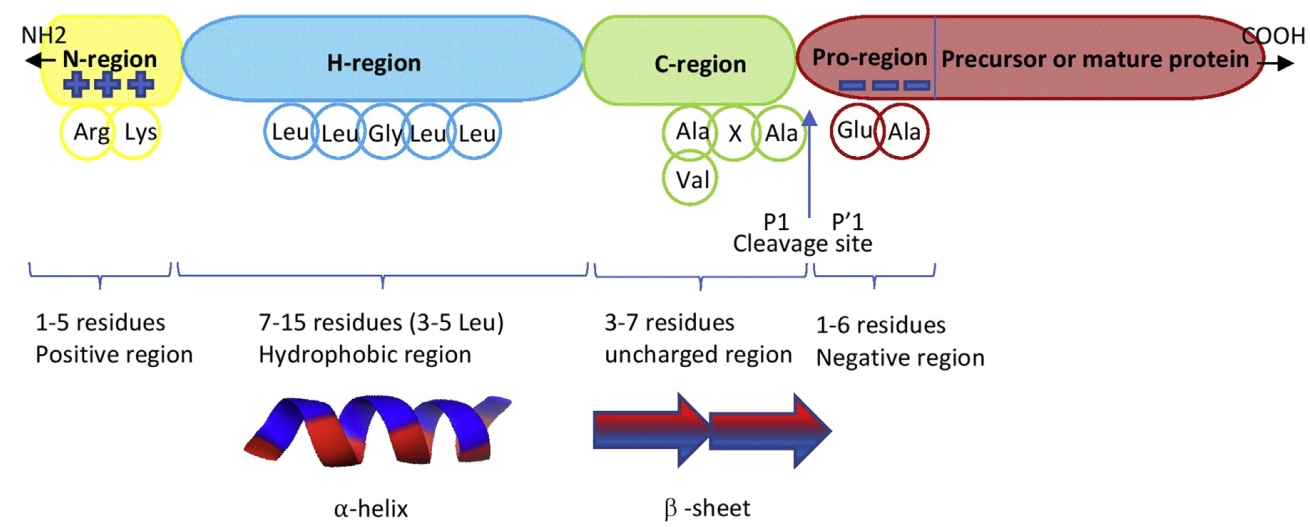
\includegraphics[width=\linewidth]
{./literature_review/subcellular_location/signal_peptides/img/signal_peptide_structure.png}
	~\end{subfigure}
	\caption{~\textbf{The general structure of a signal peptide.}
		Three general regions are discriminated inside the signal peptide and one region in the mature protein:
		(i) At the N-terminal end, there is a positively charged region, or N-region.
		(ii) This is followed by the H-region, or hydrophobic core, which forms the $\alpha$-helix.
		(iii) The C-region (C-terminal end) is where the cleavage site is situated,
		and forms a $\beta$-sheet.
		Residues before the cleavage site get a P notation,
		residues after it get a P' notation.
		The cleavage itself occurs after recognition of of the AXA or VXA motif.
		(iv) Downstream of the cleavage site, it he pro-region. 
		It is negatively charged and interacts with N-region to form a loop structure
		(from~\cite{owji2018}).}
	\label{fig:signal_peptide_structure}
~\end{figure}


			\paragraph{N-region}
				The N-region is generally around 5 residues long.
It consists mainly out of basic, positively charged side sidechains,
namely lysine, arginine and histidine.
This positive charge has multiple functions.
For a start, the positive charges interact with the negatively charged phosphate groups in the lipid layer of the plasmamembrane
(\cite{von1990}).
The balance of positive charge along the signal peptide will dictate the orientation,
thereby favoring or preventing translocation.
By having a charge difference between the C-region and N-region in favor of the latter,
the orientation of the cleavage site is more easily accessible to the SPase active site.
Additionally, the positively charged residues interact with the phosphate backbone of the SRP complex or SecB chaperone.
This interactions delays the folding process and keep the protein in transport competent state
(\cite{hardy1991}).
Interestingly, not only the amino acids composition itself,
but also translation efficiency play an important role in translocation.
In about 40 percent of the \textit{Escherichia coli} signal peptides,
the second codon is AAA (Lys).
Substitution of the codon to the lower translation-initiation-rate codon AAG has been observed to prevent secretion
(\cite{zalucki2007}).


			\paragraph{H-region}
				The hydrophobic H-region has generally a length between 7 and 15 residues and has multiple functions.
The hydrophobic residues have propensity toward forming an $\alpha$-helix.
They have a membrane spanning role,
thereby helping to orient the signal peptide.
In addition, the amino acid composition helps determining the secretory pathway, 
and protein processing (e.g. N-linked glycosylation).
In general, an increase of hydrophobicity results in higher protein translocation.
However, jamming of the translocase has been observed when hydrophobicity is increased to much,
but low hydrophobicity can slow down the translocation rate
(\cite{mordkovich2015}).
Getting the optimal balance for secretion has long been an subject of interest in protein engineering.
In Gram-negative Bacteria,
increasing the hydrophobicity augments inner membrane secretion,
but decreases outer membrane translocation.
The H-region also determines which secretory pathway the protein will end up using (Sec, SRP or Tat).
Highly hydrophobicity stabilizes the SP-SRP interactions, thus favoring the SRP pathway.
Signal peptides destined to the Tat and Sec pathway are less hydrophobic.
The role of hydrophobicity for the choice of pathway seems be more important in prokaryotes than eukaryotes,
and more significant in Gram-negative bacteria than the Gram-positive
(\cite{owji2018}).
Leucines are the most dominant residue in H-regions.
Even though the exact amino acid composition differ significantly throughout species,
conserved H-motifs are observed within the same species
(\cite{duffy2010}).
This means that signal peptides are not always interchangeable between species,
even if they have the same hydrophobicity.
Finally, H-regions often have an helix breaker present.
This enables the signal peptide to form a hairpin structure and insert itself more easily in the membrane.
Helix breakers are proline, glycine or serine residues and can be found at any position except on the edges of the H-region.

			\paragraph{C-region}
				The C-terminal part of the signal peptide or C-region contains 3-7 residues,
with five giving the best cleavage efficiency.
Amino acids of the C-region are more neutral and polar, 
and adopt a propensity toward an extended $\beta$-conformation to provide a binding site for SPase.
One of the main cleave motifs is the AXA motif (\cite{von1984}).
It is situated on positions -3 and -1 relative to the cleavage site is universal,
occurring in prokaryotic, ER, and organellar signal peptides.
Other motifs are observed for lipoproteins and prepolin (\cite{paetzel2002}).
The exact C-region features depend on the secretory pathway and species.



			\paragraph{Pro-region}
				The region located downstream from the cleavage site, but upstream from the mature protein,
is called export initiation domain pro-region.
It seems to be especially important in Bacteria 
as deletion of the pro-region will result in accumulation of protein in the cytoplasm 
and the formation of inclusion bodies.
Additionally, it affects the protein folding process.
This region can extend to a length of 30 amino acids,
but for bacterial signal peptides the first 6 residues are the most important 
as they can interact with the SPase
(\cite{auclair2012}).
It is composed of mainly neutral and acidic residues, and has therefore a negative charge.
Because of this, it interacts with the positively charged N-region to form a loop structure.
Residues near the cleavage site, especially at P1', are small and flexible 
to avoid steric hindrance when interacting with the SPase
(\cite{owji2018}).


		%\subsubsection{Secretory systems}
		%	Wim, do you think it is important about the different secretory systems (Sec, Tat, SRP).
It will take me quite some writing to get it in and while very interesting, 
I am not sure it is really necessary for the research I did.


		\subsubsection{Predicting protein location}
			The biophysical properties of signal peptides are highly conserved through evolution and present in both prokaryotes and eukaryotes.
Their presence is a clear indication that the protein in question is translocated to another subcellular location of extracellular environment.
Many predictors were designed to detect these signal peptides and their cleavage sites(\cite{armenteros2019}),
and others have included this information to predict subcellular location (\cite{jaramillo2014}).
Various machine learning techniques have been utilised for this problem including:
weight matrix methods,
hidden Markov models,
support vectors machines,
and neural networks.
For example,
SignalP 5.0 (\cite{armenteros2019}) uses a deep neural network to predict  signal peptides across all domains of life,
and in prokaryotic organisms it distinguishes between the three types (Sec/SPI; Sec/SPII; Tat/SPI).

			Even though signal peptides play an important role in protein translocation,
they are on their own insufficient to ensure this process.
Predictors like MatureP are able to separate cytoplasmic proteins from periplasmic ones 
with an AUC of 92 percent based features exclusively from the mature domains
(\cite{orfanoudaki2017}).


	\subsection{The UniProt Knowledge Database}
		With protein and nucleotide sequencing getting cheaper every year,
large-scale sequencing efforts are increasing the coverage of complete proteomes for a wider range of organisms than ever before. 
Additionally, the improvement of experimental techniques provide deeper information about structure and function of individual proteins.
The UniProt knowledgedatabase (UniProtKB) contains a wealth protein sequences and associated information.
For over half a million of these protein sequences,
expert curators have extracted detailed annotations from literature.
The UniProt Knowledgebase stores these reviewed proteins as UniProtKB/Swiss-Prot entries.
An automated pipeline, including a rule-based system, annotates the majority of unreviewed proteins.
These are stored as UniProtKB/TrEMBL entries.
UniProtKB also stores sequence clusters of 100, 90, and 50 percent identity in UniRef databases.
Finally, UniParc is the UniProt Archive and contains a complete set of the known set sequence, even those that are historically obsolete 
(\cite{uniprot2019}).

		\subsubsection{Database growth}
			The amount of protein sequences in UniProtKB has been growing exponentially from 2008 to 2018,
as shown in (Fig. \ref{fig:uniprot_growth}).
As on the moment this paragraph was written,
UniprotKB contained a total of 181,252,700 protein sequences.
562,253 were reviewed and part of the UniProtKB/Swiss-Prot database, 
the remaining 180,690,447 unreviewed sequences part of the UniprotKB/TrEMBL database.
This suggest that the exponential growth is still going on.
Translated proteomes are available for over 84 thousand different species with completely sequenced genomes.
Curators may target specific taxa to fill gabs in the taxonomic space,
and individual users can request for additional proteome imports
(\cite{uniprot2019}).


~\begin{figure}[h!]
	~\begin{subfigure}[b]{\linewidth}
		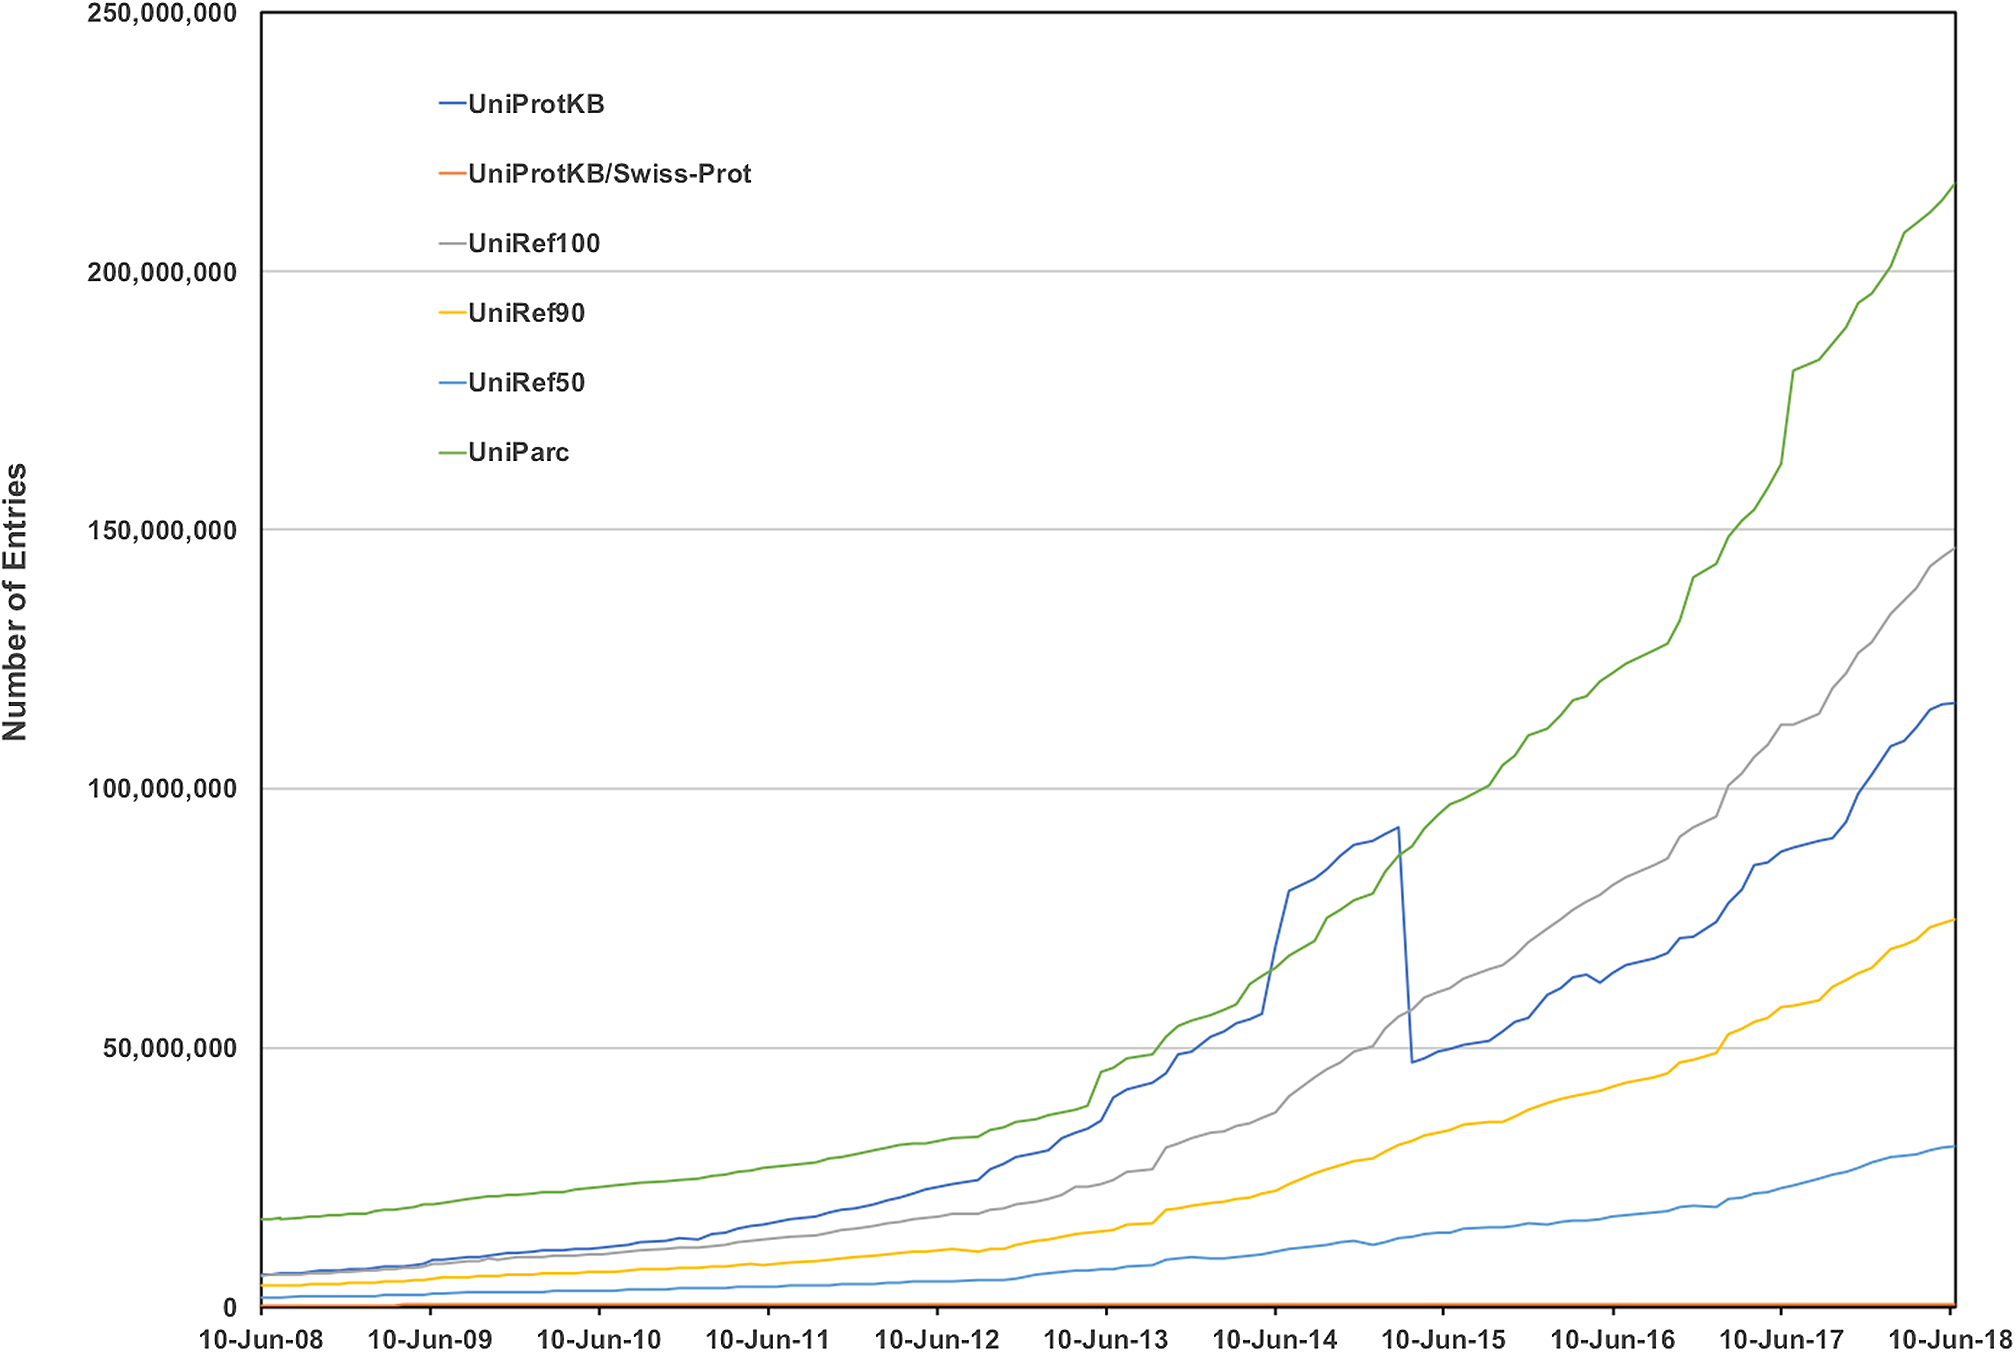
\includegraphics[width=\linewidth]
		{./literature_review/UniProtKB/database_growth/img/number_of_sequences.jpeg}
	~\end{subfigure}
	\caption{
		\textbf{Growth of UniProt sequences from 2008 to 2018.}	
		The graphs shows the growth curves of the different databases.
		Except for UniProtKB/Swiss-Prot, all databases display an overall exponential growth.
		The fall in the UniProtKB curve corresponds with a redundancy removal performed in 2015
		(from \cite{uniprot2019}).
		}
	\label{fig:uniprot_growth}
~\end{figure}


		\subsubsection{Navigation through text search}
			The standard way to access the vast magnitude of data available on UniProtKB it by using the websites text search.
The website provides a search bar in the UniProt banner in which a query can be filled in.
The query syntax accepts terms of specific fields and combines them using boolean logic.
A manual is provided on the website,
but a more convenient method is to use the query builder.
It lets the user build a query step by step by providing drop down lists for the available fields
(Fig. \ref{fig:query_builder}).
Once the 'search' button is clicked, the query is shown in the search bar in the appropriate syntax and results are given in a table like format
(Fig. \ref{fig:query_results}).
The pencil symbol lets the user choose which columns are shown.
Once satisfied, results can be downloaded in one of multiple formats, the most important being:
a fasta file of all the selected protein sequences,
an Excel or tab separated text file containing the fields of choice (e.g. id, length, and sequence) for every selected protein,
or a XML file.
The latter is not meant to be read by humans in its raw format, but can be easily parsed.
It contains all information available on UniProtKB for the selected proteins.


~\begin{figure}[h!]
	~\begin{subfigure}[b]{\linewidth}
		\centering
		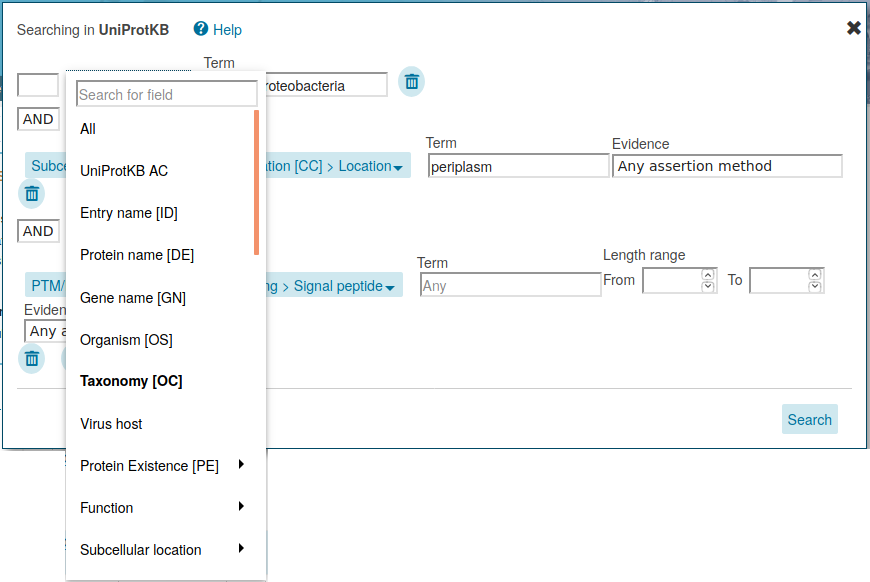
\includegraphics[width=\linewidth,height=0.3\textheight,keepaspectratio]
			{./literature_review/UniProtKB/text_search/img/query_builder.png}
		\caption{Query Builder}
		\label{fig:query_builder}
	~\end{subfigure}
	~\begin{subfigure}[b]{\linewidth}
		\centering
		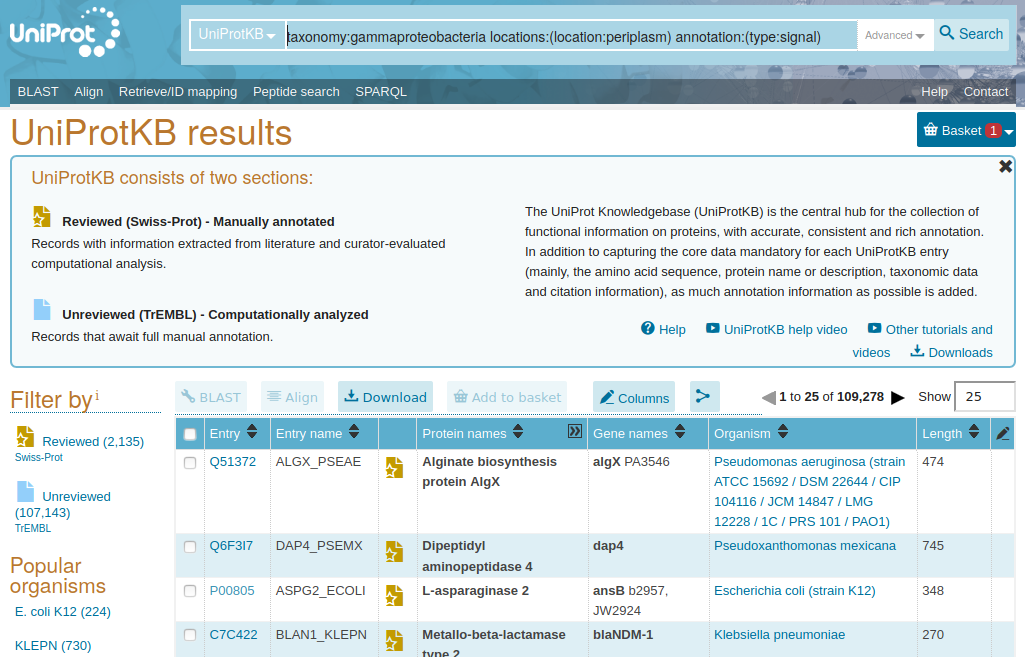
\includegraphics[width=\linewidth, height=0.5\textheight,keepaspectratio]
			{./literature_review/UniProtKB/text_search/img/query_results.png}
		\caption{Query Results}
		\label{fig:query_results}
	~\end{subfigure}
	\caption{
		\textbf{The UniProtKB website text search.}
		The vast UniProtKB database can be accessed by text search.
		\textbf{a.} The search bar accepts a boolean style of query syntax, 
		which can by build step by step with the Query Builder.
		\textbf{b.} Results are shown in a table like format.
		(Screenshot from https://www.uniprot.org/).
		}
~\end{figure}

		\subsubsection{UniProtKB REST APIs}
			The website interface is a very convenient and user friendly way to retrieve information.
Sometimes it would be useful however to access and download this in automated way.
Imagine yourself collecting all the protein sequences that have an annotation of being in the cytoplasm for 20 different organisms of interest.
For each organism, a search query would have to be entered,
the download button has to be clicked and the FASTA format selected.
Then some more clicking to specify the download location, etc.
And this has to be repeated for every of the 20 organisms. 
Now imagine that halfway you notice that UniProtKB makes the distinction 
between the "cytoplasm" and "cytosol" annotation.
Both would serve the purpose of the research however, 
so to include "cytosol" proteins, you would have to start all over again.
Easier would be to just change the query parameter and automatically iterate through all the other steps.
Another reason why someone would like to automate the retrieval process is that the database is constantly growing.
More research is being done, and curators add manual annotations.
Moreover, automatic pipelines improve in accuracy, so also unreviewed annotations get better and more abundant.
Therefore it could be useful to reuse a search query and redo an analysis with a more up to date dataset.
UniProtKB provides programmatic access to its database in the form of a set of REST APIs.
Not only is there an API to programmatically perform a query search as in the example above,
there are also REST APIs for 
retrieving individual entries,
mapping IDs from one database to another,
format conversion, 
and more
(\cite{uniprot_api}).

		\subsubsection{UniRep}
			Before a machine learning based predictor can be trained to decode biophysical features from protein sequence.
A training set needs to be created either by performing the experiments,
or by gathering publicly available data.
UniProtKB has around 180 million protein sequences available,
but only 560,000 of those are reviewed, 
potentially containing the experiments with the biophysical features that a predictor needs to learn.
This covers only 0.3 percent of the sequence space, 
meaning that most of it remains largely unexplored.
However, the knowledge that a protein exist, is already important information.
The fact that evolution has come up with a specific combination of amino acids to fulfill some (unknown) function is already important information. 
The question remains how to incorporate this into the training data.

One way to partly alleviate this limitation is by considering a protein sequence with known function or biophysical properties and assuming that sequences with a certain percentage of sequence identity will have similar biophysical features and function.
This is in fact largely what the automated annotation system of UniProtKB is based on.
One way to subsequently incorporate such evolutionary information into the predictor would be by aligning the homologues sequences into a multiple sequence alignment and take amino acid variation into account.
While such methods cover a considerably larger portion of the sequence space, 
it only works if at least one homologue has been experimentally described, and more to have some confidence.
Regions in the sequence space without any experimental information are still neglected.

\cite{alley2019} tried to use the full potential of the sequence space by training a 
multiplicative long short-term memory recurrent neural network
(mLSTM RNN) with the task of next character prediction.
To get better at this task,
the neural networks changes the weights of its hidden neurons,
effectively discovering protein features in a unsupervised way.
Since only protein sequence information needs to be known,
all regions of proteins sequence space are included in the training.
When trained, a sequence can be used as input to the neural network,
and the hidden states extracted into a fixed length vector,
which forms a semantically rich representation of the protein.
The research group called this the UniRep representation.
Humans cannot interpret this representation directly,
but machine learning methods can used it to train a predictor, 
for example for biophysical features.
Even though experimental data is still necessary for that,
the UniRep representation makes it possible for these predictions to be more generalized,
as information from the whole protein sequence space is incorporated.


\newpage

\section{Aims}
	% short rehearsal of the problem 
In order for periplasmic proteins to translocate they contain a signal peptide 
and seem to display different biophysical characteristics.
In this master thesis the difference in biophysical landscape between cytoplasmic 
and periplasmic proteins was examined by four complementary approaches.

% global approach
In the first approach,
a large dataset containing cytoplasmic and periplasmic proteins of the Gram-negative Gammaproteobacteria was extracted from UniProtKB,
and biophysical characteristics were compared.
It was examined whether periplasmic proteins are more likely to form certain secondary structures than cytoplasmic proteins.
Did they display an increased or decreased tendency toward sidechain and backbone dynamics,
and whether there were observations to indicate that periplasmic proteins fold more slowly than cytoplasmic ones.

% General comparison 
In the second approach, the same dataset and features were examined, 
but position within the protein was taken in into account.
It was examined if there was a general trend of features to appear in certain regions of the protein.
In addition, the biophysical characteristics of signal peptides was explored,
and there effect on the N-terminal regions of the mature domain of periplasmic proteins.

% twin comparison 
Evolution tends to tinker rather than invent.
This means new functionalities come into existence mostly by tweaking existing proteins, 
not by designing new ones from scratch. 
With this in mind,
there exist a whole set of proteins that homologues to each other, 
but one exist in the cytoplasm and on in the periplasm.
Such pairs will be further referred to as twins.
Interesting about these twins is that there structure and biophysical features are very similar,
and differences in characteristics are more likely related to them being in different compartments,
as that is their main difference.
Therefore, the third approach consisted of searching the UniProtKB databank for such twins and comparing there biophysical properties.
One advantage over previous approach is that twins can be directly aligned to each other,
making the differences more region specific.


% UniRep exploratory analysis
Finally, in the fourth approach it was examined how well UniRep representation could separate periplasmic proteins from cytoplasmic ones,
and whether the exclusion of the signal peptide had any effect on that.
The UniRep representation was constructed by letting a recurrent neural network explore the total of sequence space and build its own internal representation in a unsupervised way.
Therefore, it is unconstrained by mental models of the human mind, 
potentially improving classification.
This was a group project for the course "Techniques of Artificial Intelligence" in which I collaborated with 
Jessica Ody, 
Guillaume Buisson-Chavot, 
and Anthony Cnudde.

\newpage

\section{Methods}
	%\input{2.methods/2.methods.tex}
	The code and results of the analysis, as well as the script of this master thesis is available on my github.

\url{https://github.com/janvandenschilden/master_thesis}

	\subsection{UniProtKB retrieval via queries (REST API)}
		UniProtKB provides a REST API to retrieve data via queries similar to how text search works on the website interface.
The API utilises the native functionality of HTTP GET requests.
The idea is that all of the necessary information is encoded within the URL.
Subsequently a request is made to the UniProtKB server, 
which collects the data from the database, 
restructures it to the requested formatn
and sends the information back to the user.

The URL follows a certain format (shown below in the frame),
it starts with a fixed base 
(\url{https://www.uniprot.org/uniprot/?}), 
complemented  by a set of 'parameter=value' pairs.
The order of the parameters is of no importance,
and not all parameters have to be provided.
The server will fall back to default values in that case.
The \textbf{query} has a similar format to what is used by the website text search interface,
but spaces are replaced by '+' symbols.
There are different  \textbf{formats} as which the data can be downloaded:
\textit{
html,
tab,
xls, 
fasta,
gff,
txt,
xml,
rdf,
list,
and rss}.
The \textbf{columns} parameter indicates which fields should be provided in the \textit{tab} or \textit{xls} format.
The \textbf{include} parameters means different things, depending on what format was requested.
There is the possibility to Gzip the data, which is provided by the \textbf{compress} parameter.
Finally, if the user only wants N results,
it can be passed with the \textbf{limit} parameter.
By default, the counts starts from the first entry, 
but this can be changed with the \textbf{offset} parameter.


~\begin{tcolorbox}
	\url{
	https://www.uniprot.org/uniprot/?
	query=<<QUERY>>
	&
	format=<<FORMAT>>
	&
	columns=<<COLUMNS>>
	&
	include=<<yes|no>>
	&
	compress=<<yes|no>>
	&
	limit=<<LIMIT>>
	& 
	offset=<<OFFSET>>
	}
 ~\end{tcolorbox}

Implementation of the REST API was done in Python (code in Appendix section \textit{uniprotRetrieve.py}).
Datasets resulting from a query searches can easily comprise multiple gigabytes,
even more than what is available in RAM memory.
Therefore, the \textbf{requests} (\cite{reitz2012}) library was chosen to handle the HTTP GET requests,
because it has the option to retrieve data as a stream of chunks.
This allows the data to be stored on the hard disk directly, without putting a load on memory.
Sometimes the UniProtKB server is overloaded by requests and will not give anything back.
As this could break a pipeline,
the implementation was made more robust to these types of failures by
designing it to retry up to 10 attempts to do a request.
Each attempt, the program will wait an increasingly amount of time before putting a new request. 
Servers often ignore request that come in to frequently from the same origin.
Also special care was taken so that the \textbf{query} parameter can be provided in the same manner as when you would use the text search interface on the website. 
This way, a query can be gradually build up with the query builder, 
and subsequently copied as argument for in a pipeline.

	\subsection{UniProtKB database mapping (REST API)}
		UniProtKB provides a service that maps entries from one database to another.
Those databases can be internal (UniProtKB, UniRef, UniParc, etc.),
but also external (PDB, RefSeq nucleotide, Entrez Gene, etc.). 
The mapping service is both available by web interface and by programmatic access as REST API.

Code of the implementation can be found in the Appendix, section \textit{uniprotMapping.py}.
It implemented as a function that can be used in pipelines,
it accepts 7 parameters:
\textbf{
fileName,
query,
From,
To,
Format,
Columns,
and
OutputDir.
}
The \textbf{query} accepts a set of identifiers in string format, which can be separated by spaces or newline symbols.
The \textbf{From} and \textbf{To} parameters accept respectively from which database the query is mapped and to which one.
With the \textbf{Format} parameter,  different output formats can be chosen.
The parameters \textbf{fileName} and \textbf{OutputDir} indicate under what name and where the file will be stored.

It should be noted that it is better to limit the amount of identifiers per request.
Generally it is a good idea not to map more than a couple of thousand identifiers at once,
as more will tend the request to fail, 
but not always with giving an error.
Especially in the context of a pipeline, 
nothing is as frustrating than starting it to run overnight,
only to see that it failed at one of the first steps before any work was really done.
To avoid this, it is more robust to put 30 requests of 1,000 identifiers, than one request of 30,000.

	\subsection{blastp}
		Blastp  (\cite{korf2003}) is a tool that performs a local sequence alignment of a protein sequence query on a target database.
Each set of proteins (periplasmic and cytoplasmic) was clustered by organism.
Within such cluster,
the command line version of blastp (available as package for Ubuntu) was used to search for homologues between cytoplasmic and periplasmic sequences, 
in this master thesis defined as twins.
The e-value threshold was set on 1e-10.
A python wrapper was implemented to use blastp in python scripts (see appendix).

	\subsection{cd-hit}
		The bio-informatics tool cd-hit (\cite{fu2012}) clusters protein sequences by an sequence similarity threshold.
For example if a threshold of 90 percent is chosen,
the sequence identity between clusters is at most 90 percent.
Sequence identity within a cluster is more than 90 percent.
The command line version of this tool was used (as available from the Ubuntu repository).
Default parameters were used. 
The sequnece identity threshold depended on the analysis and was either 0.5 or 0.9. 
A python wrapper was written to use cd-hit in scripts (see appendix).

	\subsection{Clustal Omega}
		The command line program Clustal Omega (\cite{sievers2014}) generated the Multiple Sequence Alignments for the twins.
Default parameters were used.
Python wrapper was written to use it in scripts (see appendix).

	\subsection{EFoldMine and DynaMine biophysical predictions}
		For each protein, the following features were predicted with EFoldMine:
the propensity towards forming the different secondary structures (\textbf{helix, sheet, coil}),
the \textbf{backbone} and \textbf{sidechain} dynamics,
and the \textbf{early folding} propensity.


		A custom python script was written to map biophysical prediction to a multiple sequence alignment (see appendix),
including a function to cut signal peptides from these mapped predictions.

	\subsection{Wilcoxon-Ranksum}
		To test whether there was a significant difference between observations of two sets of data,
the Wilcoxon-ranksum test can be used.
It does not assume the data to be normally distributed,
making it more generally applicable.
The implementation of the python library \textit{scipy} was used.
It accepts two lists of observations as input,
and returns a statistic and a p-value. 
Lower p-values mean that de difference is more significant.
During the twin comparison of biophysical features, 
a threshold of 0.05 was set.

	\subsection{PCA}	
		Points in a multiple dimensional space can be fitted by a line.
The best fit can be defined as one that minimizes the the average squared distance from the points to the line.
The basis vector describing this line is called the first principal component.
The basis vector that describes the next best fitting line, orthogonal to the first is second principal component,
a third best fitting line orthogonal to both previous forms the third principal component and so on.

UniRep vectors were first scaled to a mean of 0 and standard deviation of 1 with the \textit{preprocessing} module of the \textit{sklearn} python library.
Principal components were generated with using the \textit{decomposition} module.
It uses the method of Minka,
which uses a covariance matrix.
The main goal of performing the principal component analysis in this master thesis was to visualize the 64 dimensional UniRep vectors on a 2-dimensional graph.
Visualization was done wit \textit{matplotlib}.

	\subsection{Pipeline to compare the biophysical landscape of periplasmic and cytoplasmic proteins}
		\paragraph{Scope}
			One question in the generation of a cytoplasmic and periplasmic protein dataset was on which taxonomic level to do the analysis. 
The most extensive approach would be use the UniProtKB annotation system to collect all the Bacterial proteins containing an  annotation of them being situated in the periplasm or cytoplasm.
However, since only Gram-negative Bacteria have a cytoplasm,
this would result in an uneven spread of proteins over the different taxa and introduce bias in the dataset.
Therefore,  only proteins from the class of Gammaproteobacteria were selected.
At the moment of writing, UniProtKB contained 28,310,322 protein sequences within this taxonomic group.

		\paragraph{Collecting proteins}
			The UniProtKB query retrieval REST API was utilised to download the protein sequences.
The query specified for proteins with annotations of the taxonomic class of Gammaproteobacteria, 
the desired cellular location,
and the presence or absence of a signal peptide (shown below).
Both proteins which had annotations generated by UniProtKB's automated pipelines and those backed by experimental evidence were included.
This resulted in a dataset of \textbf{1,970,892 cytoplasmic} and \textbf{109,278 periplasmic} proteins.

~\begin{tcolorbox}
Cytoplasmic:
\\
QUERY="taxonomy:Gammaproteobacteria AND (locations:(location:cytoplasm) OR locations:(location:cytosol)) NOT annotation:(type:signal)"
\\
\\
Periplasmic:
\\
QUERY="taxonomy:Gammaproteobacteria AND locations:(location:periplasm) AND annotation:(type:signal)"
~\end{tcolorbox}

		\paragraph{Reducing sequence identity}
			There is some bias towards which Bacteria are sampled for genome sequencing.
As most protein sequence information is obtained by translating these genomes,
there is also a bias in the protein sequence space.
Traditionally, only cultivatable species could be sequenced as a minimum amount of DNA was necessary for the process.
With the rise of next generation sequencing techniques, 
this has become less of a problem,
but there is still a strong sampling bias within the set of available sequences. 
Consider for example that Bacterial life has been observed on all viable ecosystems of earth, 
even up to kilometers under the ground.
However, taking a sample of the soil in the backyard is much easier than drilling a hole kilometers under ground.
As a result more soil samples are being taken than deep-earth samples.
More soil genomes have been sequenced.
This is only a very extreme case of a more general problem in the available sequence space:
for some regions there are more sequences available than others.
To avoid giving to much weight to features observed in easily sampled proteins, 
while overlooking others,
a general bio-informatics practice is to reduce sequence identity in protein sequence dataset.
Proteins obtained by the query retrieval API were reduced using cd-hit with a threshold of 50 percent sequence identity,
resulting in \textbf{30,632 cytoplasmic} and \textbf{3,883 periplasmic} proteins.

		\paragraph{Predicting biophysical features}
			For each protein, the following features were predicted with EFoldMine:
the propensity towards forming the different secondary structures (\textbf{helix, sheet, coil}),
the \textbf{backbone} and \textbf{sidechain} dynamics,
and the \textbf{early folding} propensity.


	\subsection{Pipeline for large scale cytoplasmic / periplasmic twin search}
		In this master thesis, 
a twin is defined as a pair of homologues found in the same organism,
but for which one is naturally located in the cytoplasm and the other in the periplasm.
Such twins often have similar structural and biophysical features,
but those that are different could be interesting in context of translocation.
It also allows to more closely examine the effect of signal peptides on the  biophysical landscape.

The goal of the pipeline described below (Fig. \ref{fig:twin_overview}) was to generate an extensive set of cytoplasm / periplasm twins.
This was achieved by combining the powerful annotation system of UniProtKB with standard bioinformatics tools.
To start, the query retrieval REST API was utilised to retrieve a set of cytoplasmic and periplasmic proteins, and the organisms they reside in. 
Multiple datasets were generated on different taxonomic levels ranging from the family of Enterobacteriaceae to the domain of all Bacteria.
Next, the proteins were clustered by organism and local BLAST search of cytoplasmic against periplasmic proteins was performed to identify homologues twins.
To look at the twins in an evolutionary relevant context,
more distant homologues were retrieved and two multiple sequence alignments were generated for each twin
(one for the cytoplasmic and one for the periplasmic protein).
Traditional methods to search for homologues such as BLAST (\cite{johnson2008})
and 
JackHMMer (\cite{johnson2010})
are to slow to use on large scale.
Additionally, I could not find an API to automate the process.
Therefore the UniProtKB mapping REST APA was utilised to obtain the UniRef50 clusters.
All members within a clusters have at least 50 percent sequence identity.
Subsequently, 
cd-hit (\cite{li2006}) clustered the UniRef50 members to a sequence identity threshold of 90 percent threshold to reduce sampling bias.
Finally, ClustalOmega (\cite{sievers2014}) generated a MSA from these members with at most 90 percent sequence identity.

~\begin{figure}[h!]
	~\begin{subfigure}[b]{\linewidth}
		\centering
		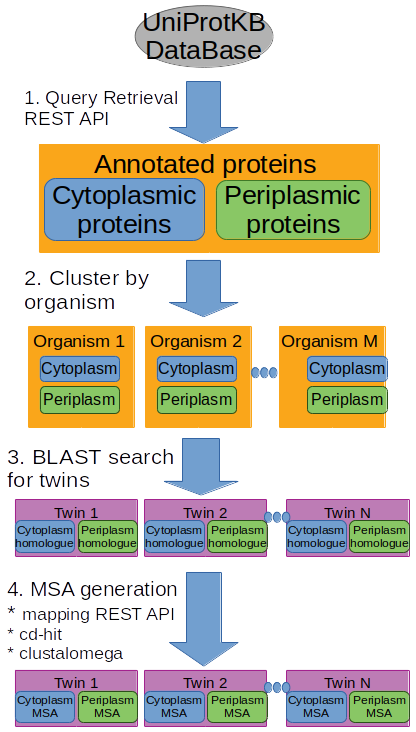
\includegraphics[width=\linewidth, height=0.6\textheight, keepaspectratio]
		{./methods/pipeline_twin_search/img/generalFigure.png}
	~\end{subfigure}
	\caption{
		\textbf{General overview of the cytoplasm / periplasm twin search.}
	}
	\label{fig:twin_overview}
~\end{figure}


		\subsubsection{UniProtKB query retrieval REST API}
			When retrieving proteins with the query retrieval REST API, 
it can be specified which features should be present (or absent).
For the cytoplasm proteins, only proteins having an annotation of being located in the cytoplasm or cytosol were kept.
As additional check, no signal peptides could be present.
For the periplasmic proteins, the query asked for proteins with an annotation being located in the periplasm.
In addition, a signal peptides should be present.

Only Gram-negative Bacteria contain a periplasm. 
However, Gram-negative Bacteria are not a monophylogenetic taxonomic group.
Therefore, multiple datasets were generated on different taxonomic levels:
\textit{
Enterobacteriaceae,
Enterobacterales,
Gammaproteobaceria,
Proteobacteria,
}
and \textit{Bacteria}.
As example, a typical search query is shown below.
Proteins were downloaded in \textbf{tab}-format with the following \textbf{columns}:
\textit{
	id,
	organism,
	ec,
	sequence
}

~\begin{tcolorbox}
	\textbf{Cytoplasmic proteins:}

	QUERY="taxonomy:Bacteria (locations:(location:cytoplasm) OR locations:(location:cytosol)) NOT annotation:(type:signal)"
	\\
	\\
	\textbf{Periplasmic proteins:}

	QUERY="taxonomy:Bacteria locations:(location:periplasm) annotation:(type:signal)"
~\end{tcolorbox}

In addition to previous searches, 
it would be interesting to know for which twins there were PDB structures available.
Therefore, a similar query search was performed as described above, but with the extra limitation
(shown below).

~\begin{tcolorbox}
	\textbf{Cytoplasmic proteins:}

	QUERY="taxonomy:Bacteria database:(type:pdb) (locations:(location:cytoplasm) OR locations:(location:cytosol)) NOT annotation:(type:signal)"
	\\
	\\
	\textbf{Periplasmic proteins:}

	QUERY="taxonomy:Bacteria locations:(location:periplasm) annotation:(type:signal) database:(type:pdb)"
~\end{tcolorbox}

 The query on all Bacteria resulted in \textbf{7,772,586 cytoplasmic} and 
 \textbf{171,333 periplasmic} proteins. 
 It should be noted that the phylum of Proteobacteria already contained 169,484 of the periplasmic proteins,
making it the largest Gram-negative group.

		\subsubsection{Cluster proteins by organism}
			The \textit{tab} files generated in previous step contain for each protein 
the UniProtKB identifier,
the organism the protein originates from,
and the protein sequence.
A custom python script (for code see appendex sections \textit{clusterByOrganism.py}) clustered the proteins of the same organism together, 
and generated two \textit{fasta} files for each organism.
One containing the periplasmic proteins and one containing the cytoplasmic proteins.

		\subsubsection{Search for twins using blastp}
			To search for twins, the command line \textit{blastp} tool was used from the \textbf{ncbi-blast+} package.
The general syntax for the tool is given below.

~\begin{tcolorbox}
	blastp -query $<<$QUERY.FASTA$>>$ -db $<<$DATABASE$>>$ -evalue $<<$EVALUE$>>$
~\end{tcolorbox}

A database can be generated from a fasta file with following command.

~\begin{tcolorbox}
	makeblastdb -in $<<$FASTA$>>$ -dbtype 'prot' -out $<<$DATABASE$>>$
~\end{tcolorbox}

Custom Python wrapper function were written for those two commands
(for code see Appendex section \textit{generateDatabases.py} and \textit{runBlast.py}).

For each organism, a database was generated using the periplasm \textit{fasta} file.
Against this database the, cytoplasm \textit{fasta} file was searched for homology detection.
As threshold, an e-value of 1e-10 was chosen.
Finally, a custom parser (for code appendix section \textit{extractTwinsFromBlast.py})
extracted the twins for the \textit{blast} file format to a simple \textit{tab} file.
Within this file, each row represents a twin, one columns contains the identifier of the cytiplasmic protein, one the identifier of the periplasmic protein.
In total, \textbf{31,165 twins} were found,
spread over \textbf{780 different organisms}.

		\subsubsection{Further filter and processing steps}
			For each periplasmic protein, signal peptide start and end were retrieved with the UniProtKB mapping API.
In addition, cytoplasmic and periplasmic proteins were mapped to their UniRef50 clusters.
Also the protein lengths were retrieved,
and for each twin the absolute difference in lengths and relative ratio was calculated.
Twins were the ratio of the length of the largest protein divided by the length of the smallest protein was smaller than 0.75,
were removed from the dataset, resulting in remaining \textbf{19,913 twins}.

To look at twins from an evolutionary point of view, 
a multiple sequence alignment (MSA) would have to be generated.
Homologues have to be searched to generate such MSA,
and many of these homologues are likely to be twins themselves in another organism, thus already in the dataset.
Therefore twins were clustered by their UniRef50 group.
This resulted in \textbf{16 UniRef50 clustered Twins} (Table. \ref{table:twins}).
To show the importance of this clustering step,
consider the following:
\textbf{19,555} out of the \textbf{19,913} are part of the UniRef50\_P62602-UniRef50\_Q8XDH7 twin cluster.
If protein sequences were to be used without prior clustering,
any signal that would have come out of the analysis would be strongly biased toward this twin cluster.
Specific mechanisms observed for that specific twin would be mistaken for more general mechanism of protein export.

~\begin{longtable}[]{@{}lllllll@{}}
\toprule
& Cytoplasm uniref50 & cluster size & Periplasm uniref50 & cluster size \tabularnewline
\midrule
\endhead
0 & UniRef50\_Q2NVU4 & 124 & UniRef50\_A0A1X1D1X1 & 148 \tabularnewline
1 & UniRef50\_P83221 & 4189 & UniRef50\_O53021 & 2118 \tabularnewline
2 & UniRef50\_Q96VT4 & 1678 & UniRef50\_O59651 & 9906 \tabularnewline
3 & UniRef50\_P0A963 & 3836 & UniRef50\_P00805 & 2537 \tabularnewline
4 & UniRef50\_P0AAL2 & 1270 & UniRef50\_P0AAL4 & 492 \tabularnewline
5 & UniRef50\_P10902 & 6730 & UniRef50\_P0C278 & 160 \tabularnewline
6 & UniRef50\_P21517 & 4496 & UniRef50\_P25718 & 5447 \tabularnewline
7 & UniRef50\_O33732 & 29 & UniRef50\_P39185 & 6749 \tabularnewline
8 & UniRef50\_P44650 & 243 & UniRef50\_P44652 & 304 \tabularnewline
9 & UniRef50\_P0A9L3 & 1427 & UniRef50\_P45523 & 2225 \tabularnewline
10 & UniRef50\_P12994 & 1160 & UniRef50\_P77368 & 1614 \tabularnewline
11 & UniRef50\_Q8ZRT8 & 1014 & UniRef50\_Q32JZ5 & 878 \tabularnewline
12 & UniRef50\_Q72CB8 & 24 & UniRef50\_Q72EC8 & 17 \tabularnewline
13 & UniRef50\_A0A432R1Z2 & 206 & UniRef50\_Q7M827 & 379 \tabularnewline
14 & UniRef50\_P62602 & 2175 & UniRef50\_Q8XDH7 & 3943 \tabularnewline
15 & UniRef50\_Q32JZ5 & 878 & UniRef50\_Q8ZRT8 & 1014 \tabularnewline
\bottomrule
\caption{\textbf{Twins of UniRef50 clusters.}
Table shows twins of UniRef50 clusters with cluster size next to it.
Each twin of clusters contains at least one pair of twin proteins within the same organism.}
\label{table:twins}
~\end{longtable}

For each clusters, members were retrieved with UniRepKb mapping API,
and sequence identity was reduced with cd-hit (threshold 0.9).
A msa was generated with Clustal omega.
Biophysical features were predicted using DynaMine and EFoldMine,
for the periplasmic proteins, this was repeated with and without signal peptide.
For each twin and for every aligned position, the Wilcoxon-Ranksum was utilised to see where the distributions of biophysical properties differed significantly (threshold 0.05).
For each position when there were significant differences in distribution, medians were determined for both the cytoplasmic and periplasmic proteins, and the difference in medians was stored in a list per position.
This means that each position could have at most 16 values (one for each twin).
Of these values, the median and quartiles were calculated and plotted.


	\subsection{UniRep based analysis}
		Before a machine learning based predictor can be trained to decode biophysical features from protein sequence.
A training set needs to be created either by performing the experiments,
or by gathering publicly available data.
UniProtKB has around 180 million protein sequences available,
but only 560,000 of those are reviewed, 
potentially containing the experiments with the biophysical features that a predictor needs to learn.
This covers only 0.3 percent of the sequence space, 
meaning that most of it remains largely unexplored.
However, the knowledge that a protein exist, is already important information.
The fact that evolution has come up with a specific combination of amino acids to fulfill some (unknown) function is already important information. 
The question remains how to incorporate this into the training data.

One way to partly alleviate this limitation is by considering a protein sequence with known function or biophysical properties and assuming that sequences with a certain percentage of sequence identity will have similar biophysical features and function.
This is in fact largely what the automated annotation system of UniProtKB is based on.
One way to subsequently incorporate such evolutionary information into the predictor would be by aligning the homologues sequences into a multiple sequence alignment and take amino acid variation into account.
While such methods cover a considerably larger portion of the sequence space, 
it only works if at least one homologue has been experimentally described, and more to have some confidence.
Regions in the sequence space without any experimental information are still neglected.

\cite{alley2019} tried to use the full potential of the sequence space by training a 
multiplicative long short-term memory recurrent neural network
(mLSTM RNN) with the task of next character prediction.
To get better at this task,
the neural networks changes the weights of its hidden neurons,
effectively discovering protein features in a unsupervised way.
Since only protein sequence information needs to be known,
all regions of proteins sequence space are included in the training.
When trained, a sequence can be used as input to the neural network,
and the hidden states extracted into a fixed length vector,
which forms a semantically rich representation of the protein.
The research group called this the UniRep representation.
Humans cannot interpret this representation directly,
but machine learning methods can used it to train a predictor, 
for example for biophysical features.
Even though experimental data is still necessary for that,
the UniRep representation makes it possible for these predictions to be more generalized,
as information from the whole protein sequence space is incorporated.


	\subsection{Visualization}
		Graphs were generated with the python library \textit{matplotlib} (\cite{hunter2007})
and \textit{seaborn} (\cite{bisong2019}).
Tables were generated in the python library \textit{pandas},
exported as html, 
and parsed to tex syntax with the command line tool \textit{pandoc}.
Flowcharts were created with \textit{LibreOffice Draw}.
Sources were provided for images created by other authors.


\newpage

\section{Results and discussion}
	\subsection{General comparison of the biophysical landscape between cytoplasmic and periplasmic proteins}
		\input{./results/general_comparison/intro.tex}
		\subsubsection{Global feature comparison}
			\input{./results/general_comparison/intro.tex}
			\paragraph{Protein length}
				Both cytoplasmic and periplasmic proteins seem to have a maximum in distribution around the length of 220,
and both distribution display an positive skewness toward larger proteins lengths (Fig. \ref{fig:protein_lengths_graph})
The cytoplasmic distribution is more evenly spread around a wider range of protein lengths.
The periplasmic distribution on the other hand displays sharper peaks.
On average, 
periplasmic proteins are shorter than cytoplasmic ones,
as was determined with a Wilcoxon-ranksum test (p-value 2e-24).
This difference in length was also observed by \cite{loos2019} in \textit{Escherichia coli},
but seems to hold true for Gammaproteobacteria in general.
The maximum length observed in cytoplasmic proteins was 3326,
for periplasmic proteins this was only 1849 (Fig. \ref{fig:protein_lengths_table}).
Additionally, the histogram shows that protein with a length higher than 600 occur more frequently in the cytoplasm than periplasm.

~\begin{figure}[h!]
	~\begin{subfigure}[b]{0.3\linewidth}
		~\begin{longtable}[]{@{}lll@{}}
			\toprule
			& Cytoplasm & Periplasm\tabularnewline
			\midrule
			\endhead
			count & 30632 & 3883\tabularnewline
			mean & 336 & 286\tabularnewline
			std & 212 & 125\tabularnewline
			min & 42 & 78\tabularnewline
			25\% & 200 & 213\tabularnewline
			50\% & 283 & 244\tabularnewline
			75\% & 409 & 330\tabularnewline
			max & 3326 & 1849\tabularnewline
			\bottomrule
		~\end{longtable}
		\caption{}
		\label{fig:protein_lengths_table}
	~\end{subfigure}
	\hfill
	~\begin{subfigure}[b]{0.68\linewidth}
		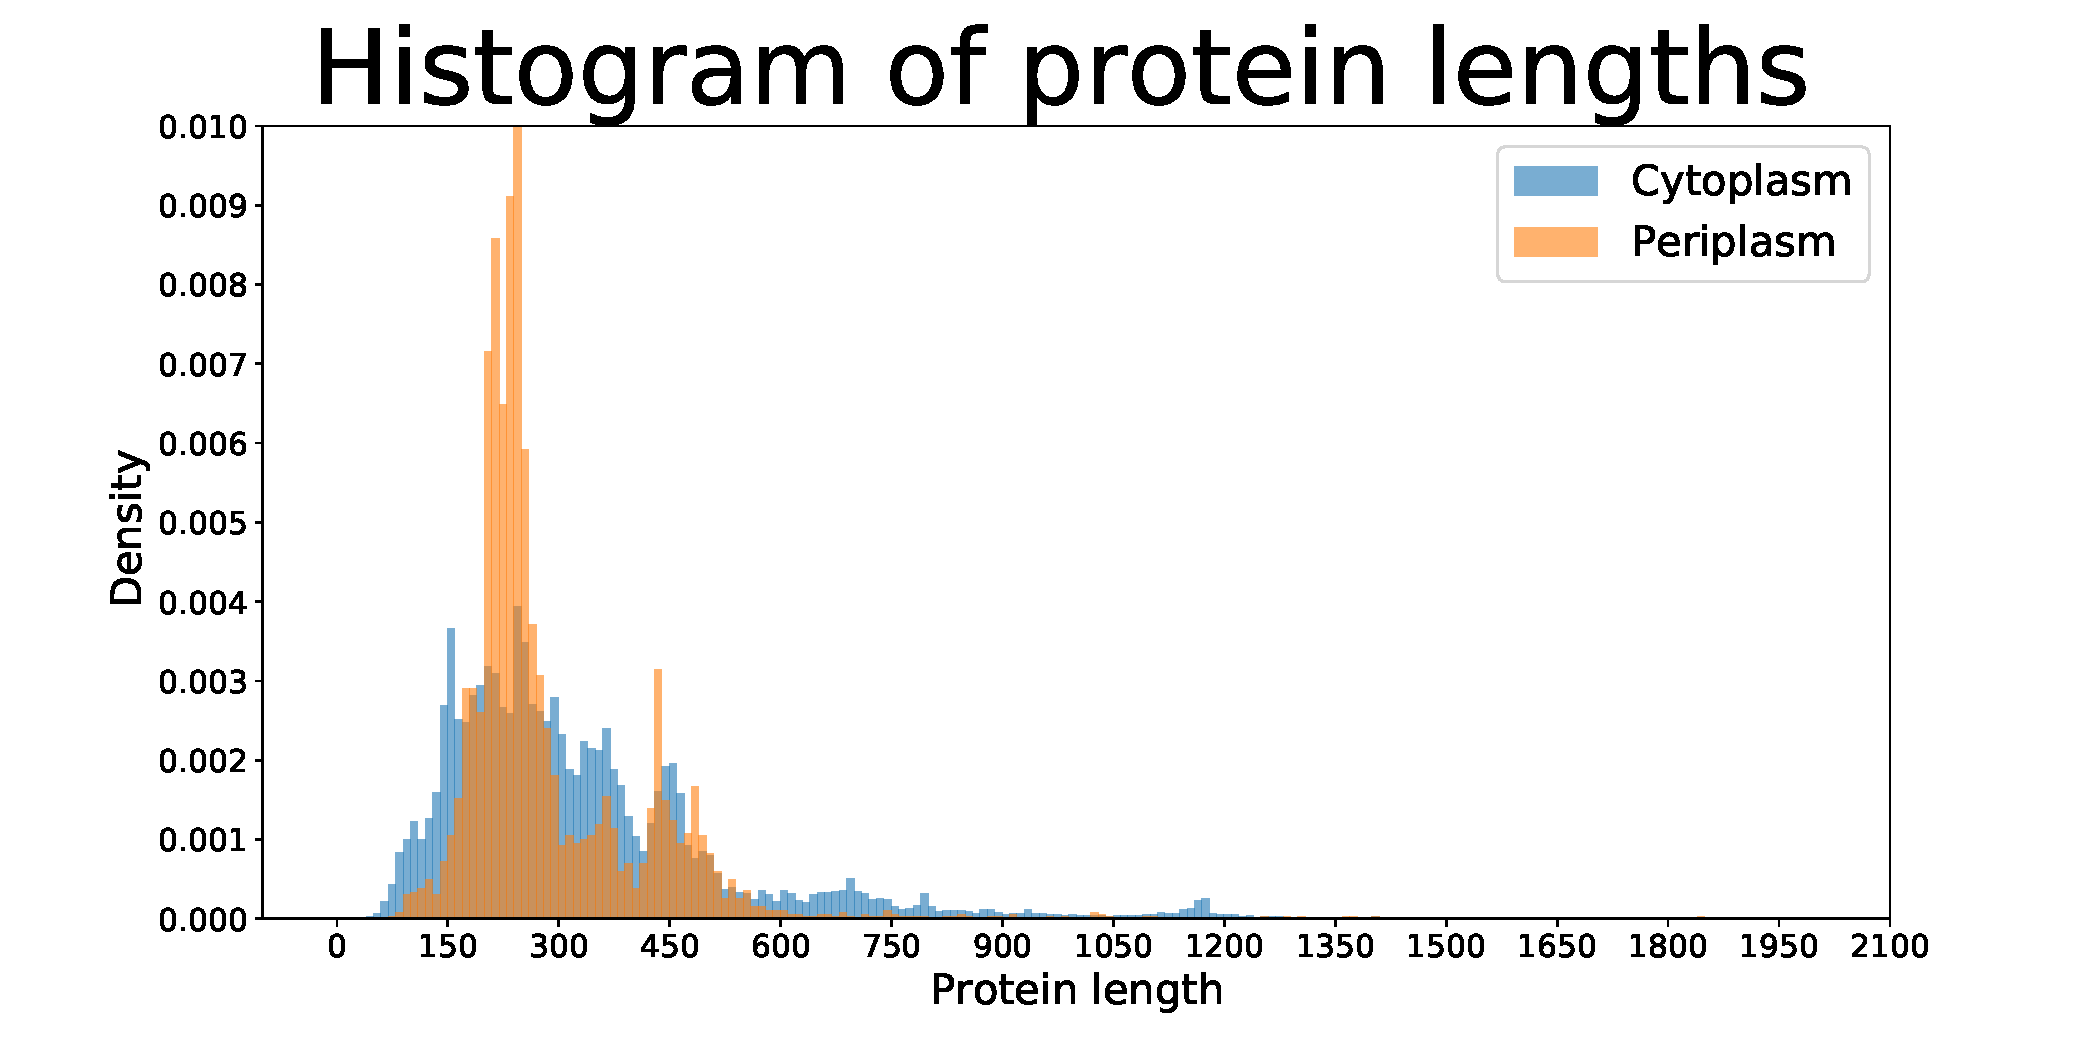
\includegraphics[width=\linewidth]
{./results/general_comparison/global_comparison/length/img/protein_lengths.pdf}
		\caption{}
		\label{fig:protein_lengths_graph}
	~\end{subfigure}
	\caption{
	\textbf{Comparison of protein length distributions between cytoplasmic and periplasmic proteins.}
	}
	\label{fig:protein_lengths}
~\end{figure}

			\paragraph{Amino acid composition}
				Fig. \ref{fig:amino_acid_composition} compares the amino acid composition.
Some very similar preferences were observed in the Gammaproteobacteria when compared to \textit{Escherichia coli} as reported by \cite{loos2019}.
Cytoplasmic proteins are enriched in 
charged, and larger acyclic hydrophobic residues (Leu and Ile).
Periplasmic proteins on the other hand display a preference for polar and small hydrophobic residues (Ala, Val).
There are also some differences:
where \cite{loos2019} observed a preference for aromatic residues in the cytoplasmome,
this is not the case for this dataset.
However, it should be noted that this dataset only comprises periplasmic proteins,
whereas their set also contained those proteins that are fully excreted in the surrounding milieu.


~\begin{figure}[h!]
	\centering
	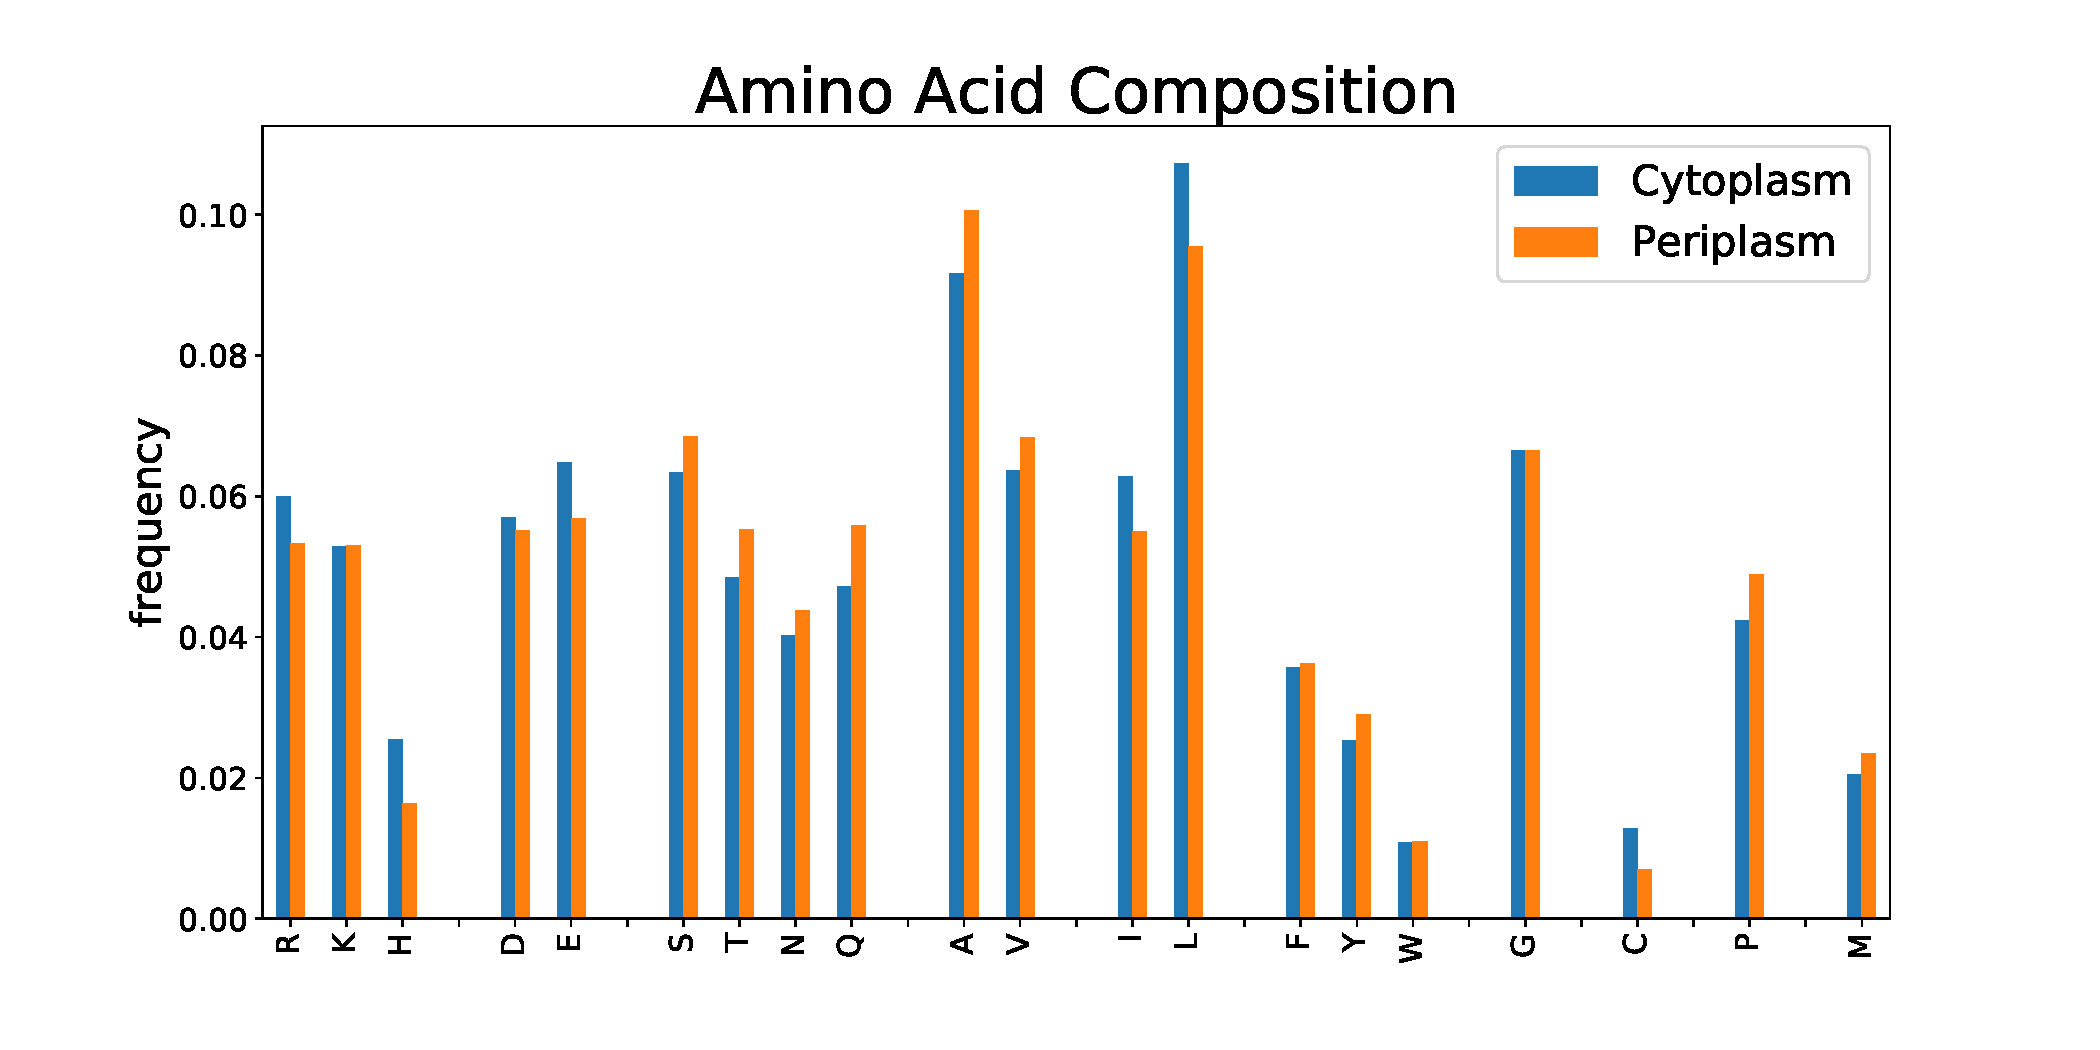
\includegraphics[width=\linewidth]{./results/general_comparison/global_comparison/amino_acid_composition/img/amino_acid_composition.pdf}
	\caption{\textbf{Amino acid composition in periplasmic and cytoplasmic proteins.}}
	\label{fig:amino_acid_composition}
~\end{figure}

			\paragraph{Global biophysical feature comparison}
				Comparison between the global biophysical features (Fig. \ref{fig:global_biophysical}) 
shows that periplasmic proteins have an higher tendency toward sheet and coil formation,
but lower tendency towards helix formation when compared to cytoplasmic proteins. 
In addition, they show more sidechain and backbone dynamics,
and a decreased tendency towards early folding.

~\begin{figure}[h!]
	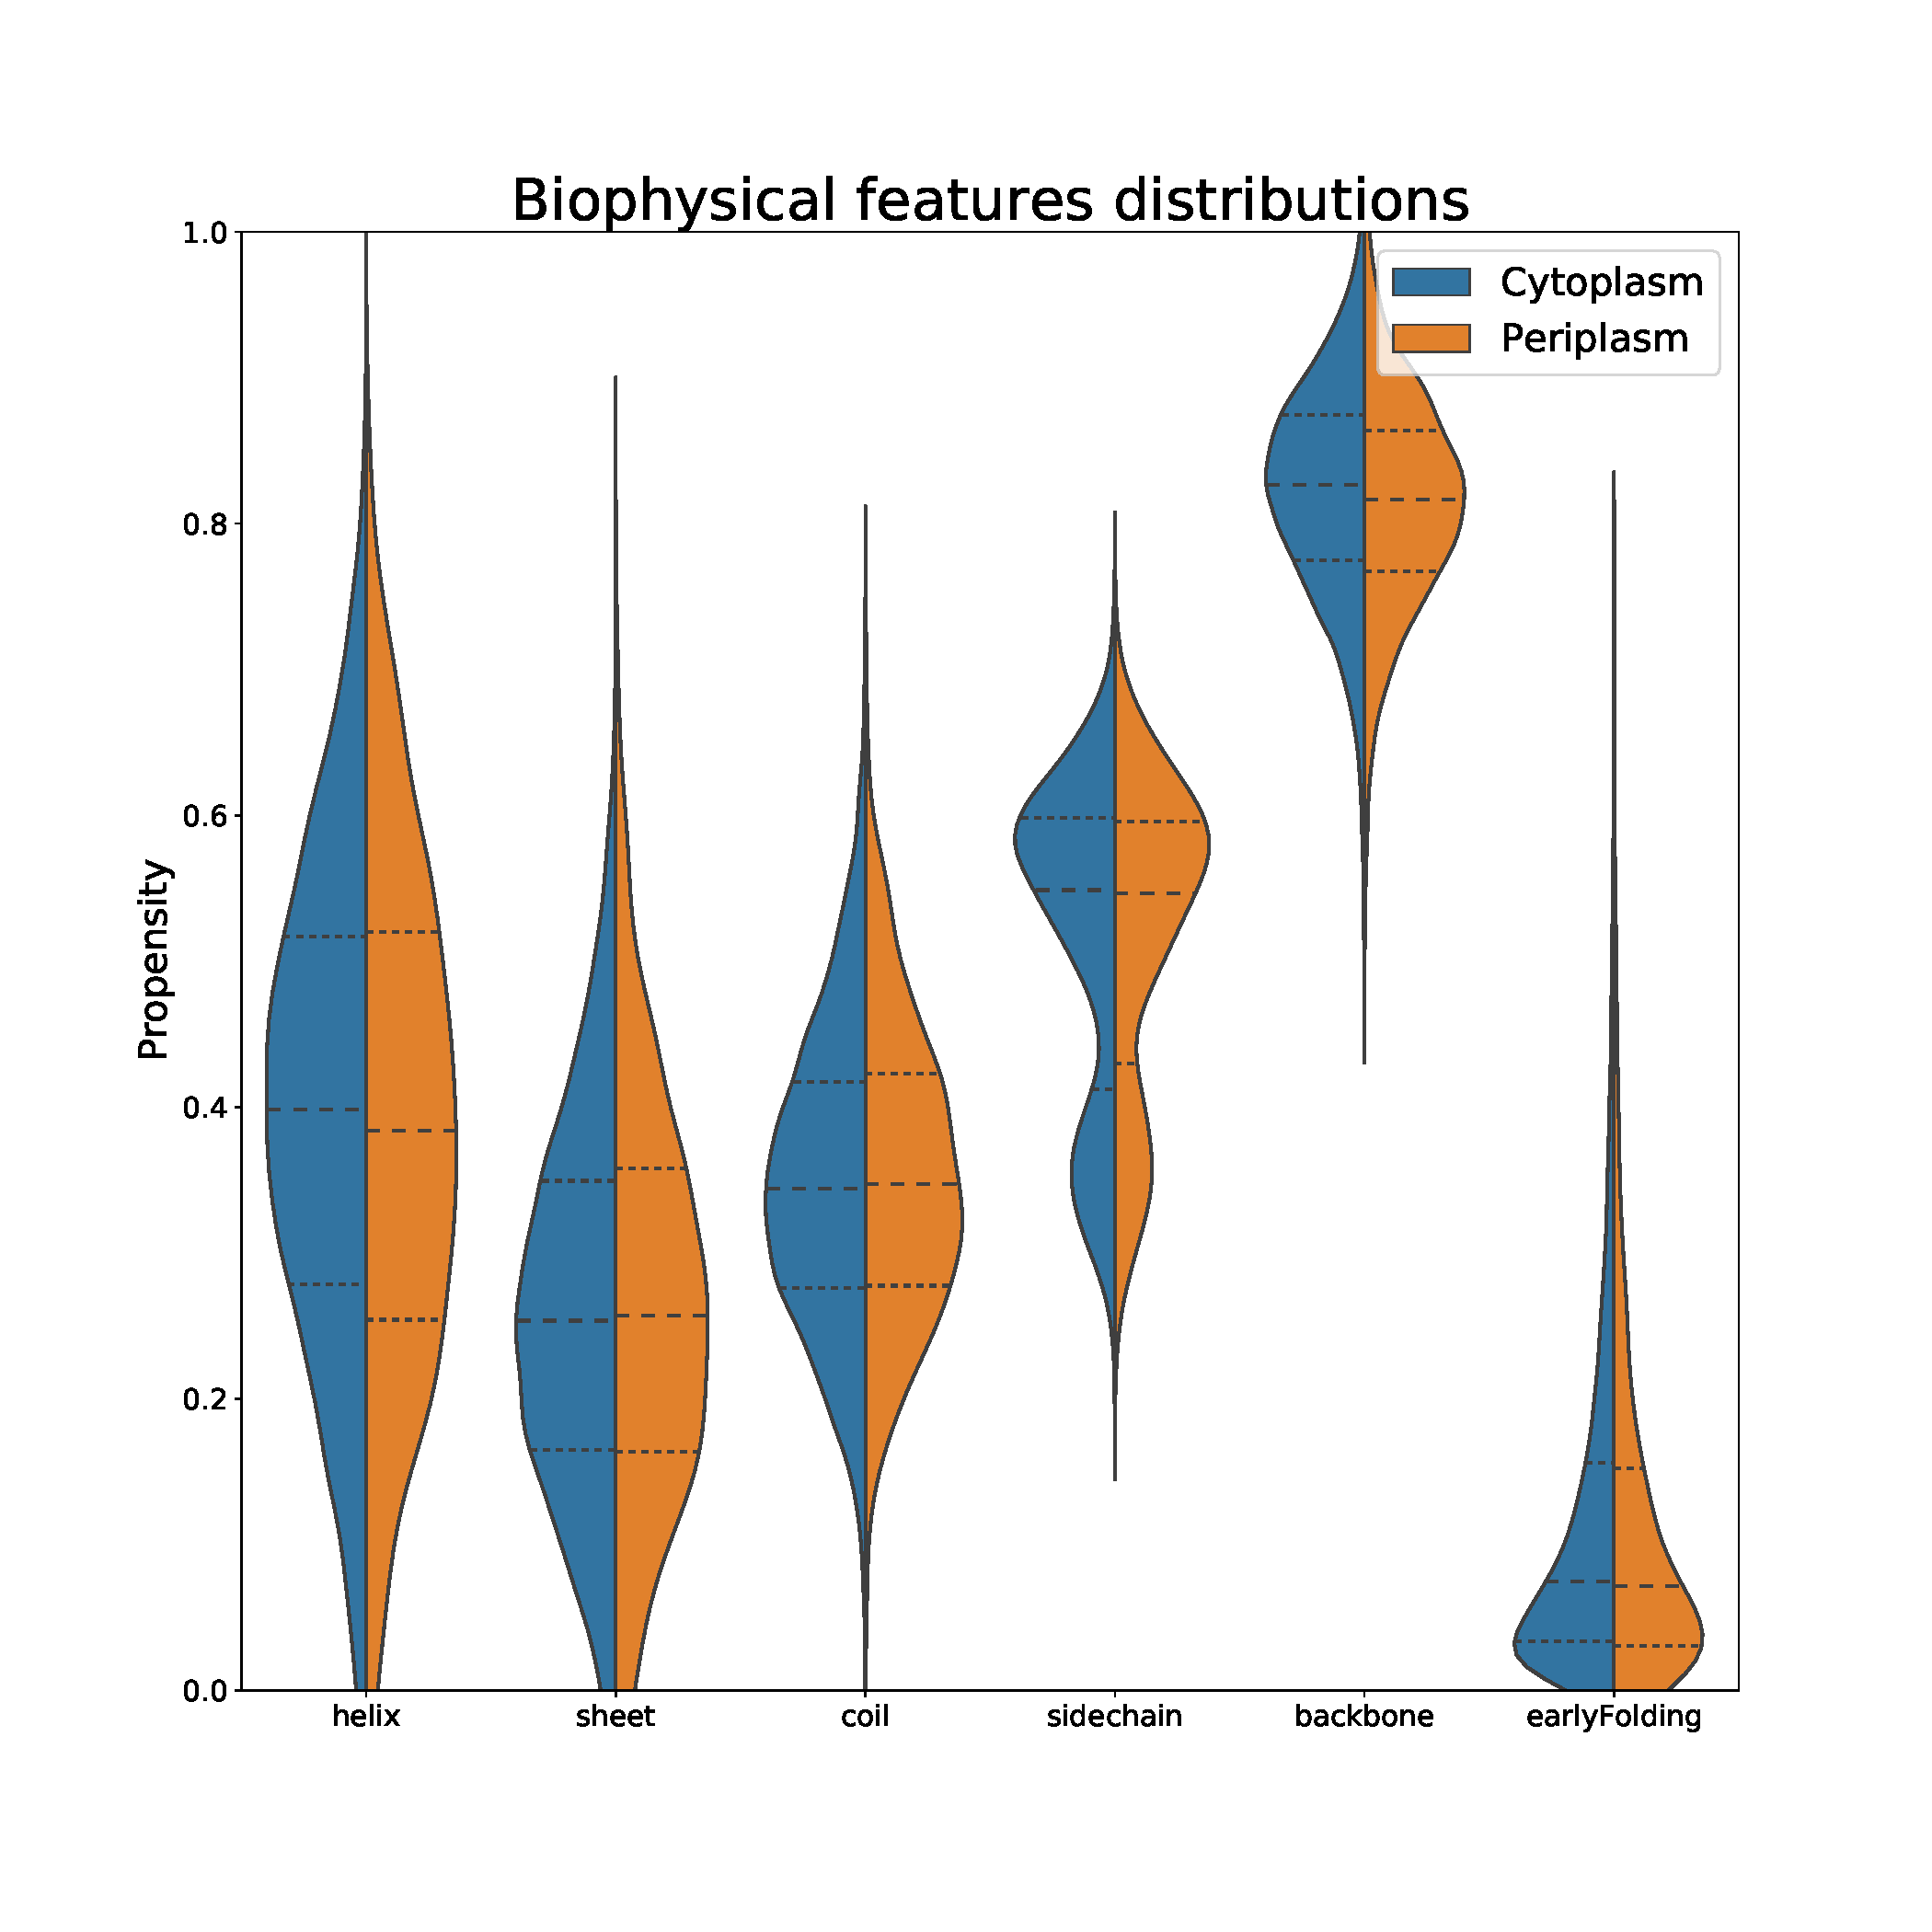
\includegraphics[width=\linewidth]{./results/general_comparison/global_comparison/biophysical/img/features_violin.pdf}
	\caption{
		\textbf{Comparison between the biophysical propensity distributions of cytoplasmic and periplasmic proteins.}
		Propensities toward 
		\textit{helix,
		sheet,
		coil,
		sidechain,
		backbone,}
		and
		\textit{earlyFolding}
		were predicted by EFoldMine and DynaMine.
		In total there were 11,424,793 residues (each with a predicted propensity toward the biophysical features described above) spread over 30,632 cytoplasmic  and 3,883 periplasmic proteins.
		In general, the distribution have a similar shape,
		but differences are significant, P-value determined by the Wilcoxon-ranksum test.
		Periplasmic as compared to cytoplasmic proteins tend to have
		less propensity toward helical formation (P-value 0.0),	
		but increased propensity toward sheet (P-value 4e-57) and coil (P-value 9e-252) formation.
		They have an increased sidechain (P-value 2e-9) and backbone (P-value 0.0) dynamics,
		and a decreased propensity toward early folding (P-value 0.0).
		}
	\label{fig:global_biophysical}
~\end{figure}

		\subsubsection{Local feature comparison}
			In the previous section, global biophysical features were compared between cytoplasmic and periplasmic proteins.
In this section, it is examined how those features change with respect to the location within the protein, 
and how signal peptides can have an effect on those features.


			
For each residue of every protein, 
the following 6 biophysical features were predicted:
\textit{
helix,
sheet,
coil,
sidechain dynamics,
backbone dynamics},
and
\textit{early folding propensity}.
For every residue position,
the median, first and third quartile of every biophysical prediction was calculated.
This was done seperately for the cytoplasmic proteins,
periplasmic proteins,
and again for the periplasmic proteins but with the signal peptide cut off.
For example,
there are 30,632 cytoplasmic proteins in the dataset, thus 30,632 first residues. 
Each of these residues can have a different local environment, so different biophysical predictions.
The median and quartiles are then calculated for these 30,632 values and plotted on a graph.
This is repeated for all different residue positions, generating a continuous box-plot.
Similarly, medians and quartiles are calculated for the periplasmic proteins, one time with signal peptide and one time without.
Signal peptides are indicated by a negative residue position.
Because the proteins within this dataset have at most 50 percent sequence identity, 
protein specific tendencies will be averaged out.
Only very general position specific propensities that are true for most proteins will be detected.
Therefore, only the first 70 residues of the mature domain are shown in the graphs below.
Similarly, the general effect of the signal peptide on its local sequence environment is shown.

			~\begin{figure}[h!]
	~\begin{subfigure}[b]{\linewidth}
		\centering
		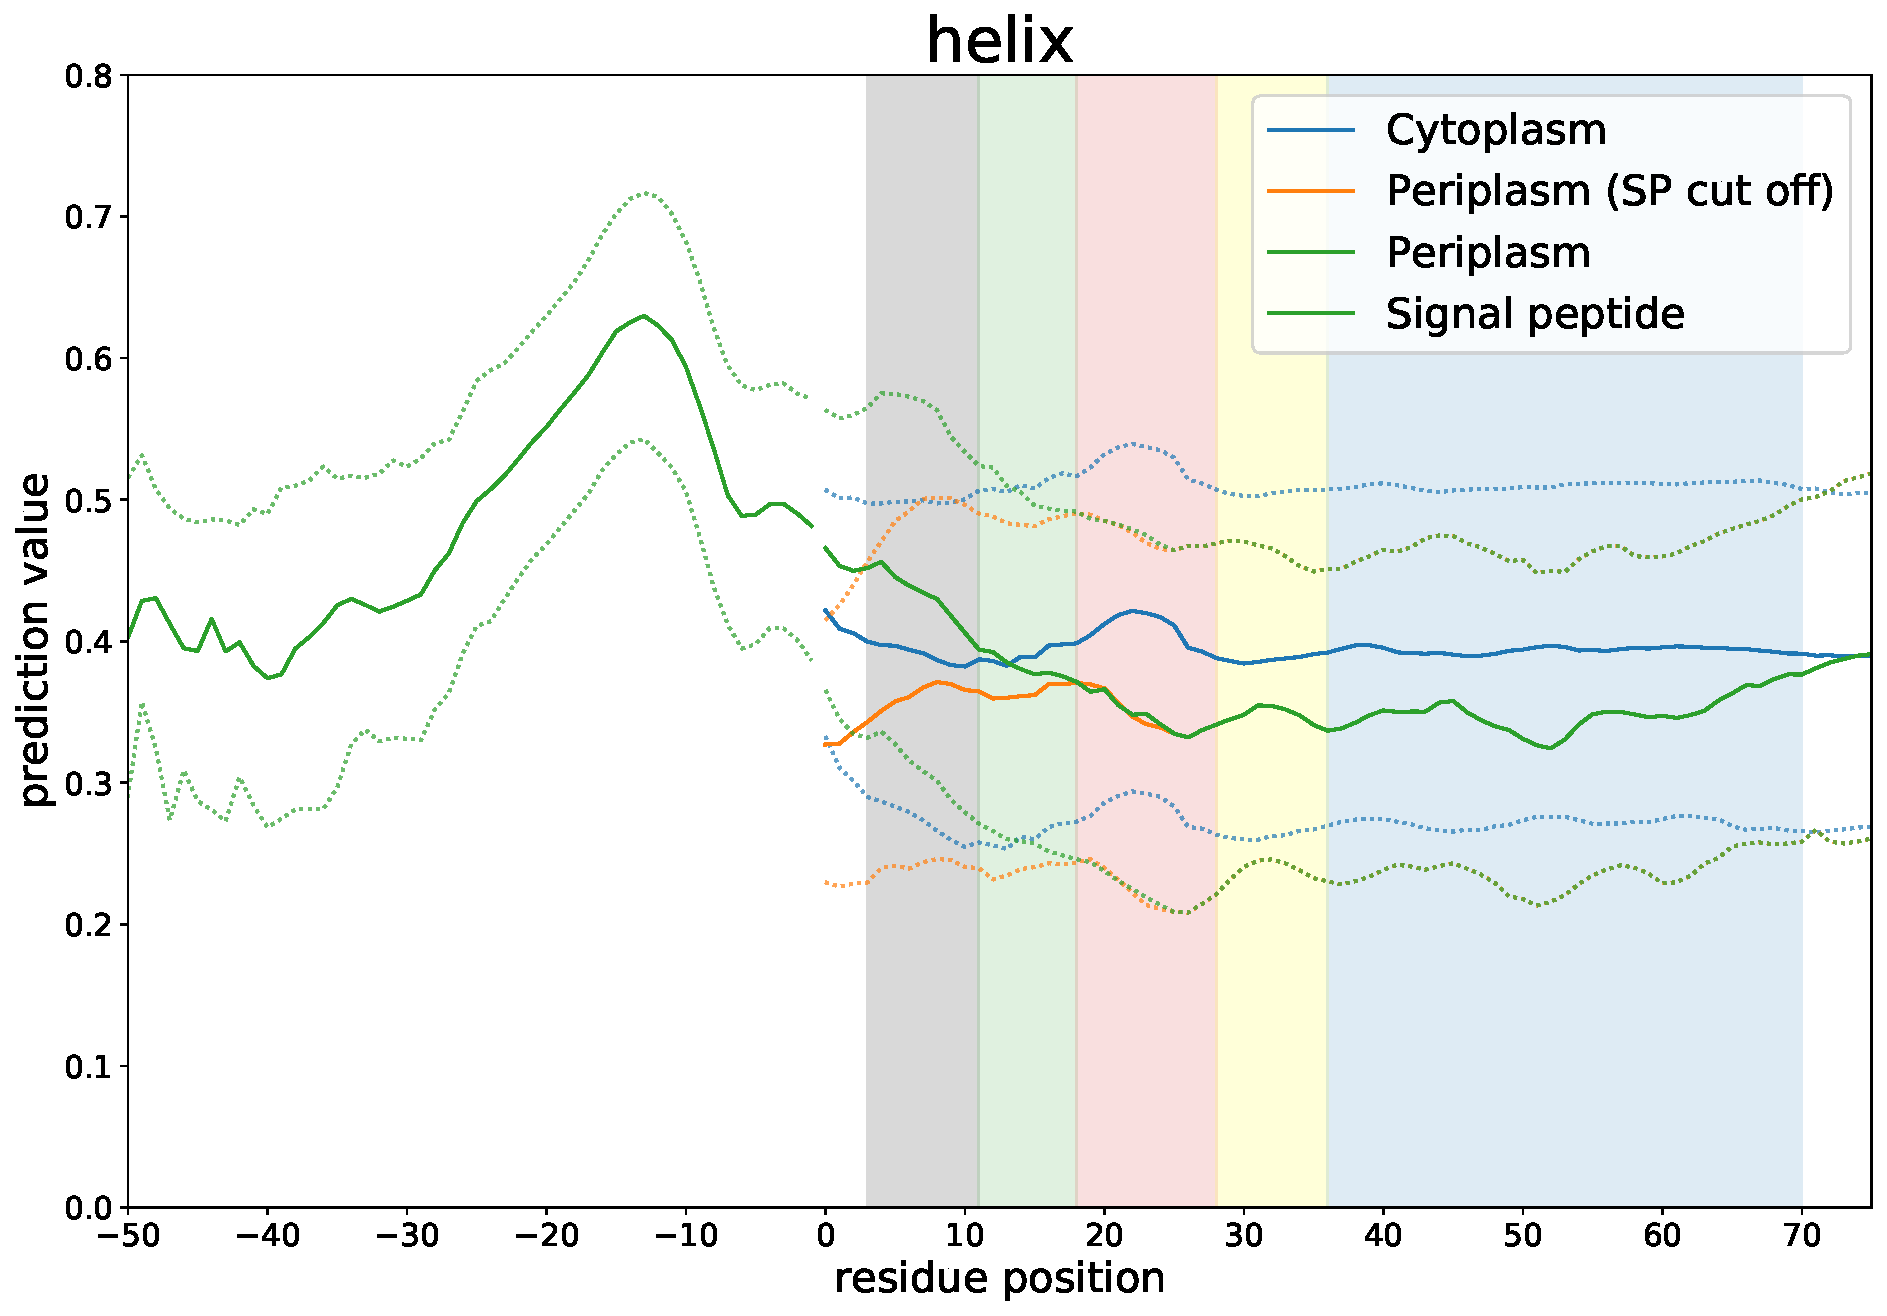
\includegraphics[width=\linewidth, height=0.46\textheight, keepaspectratio]{./results/general_comparison/local_comparison/img/local_helix.pdf}
		\label{fig:local_helix}
	~\end{subfigure}
	\newline
	~\begin{subfigure}[b]{\linewidth}
		\centering
		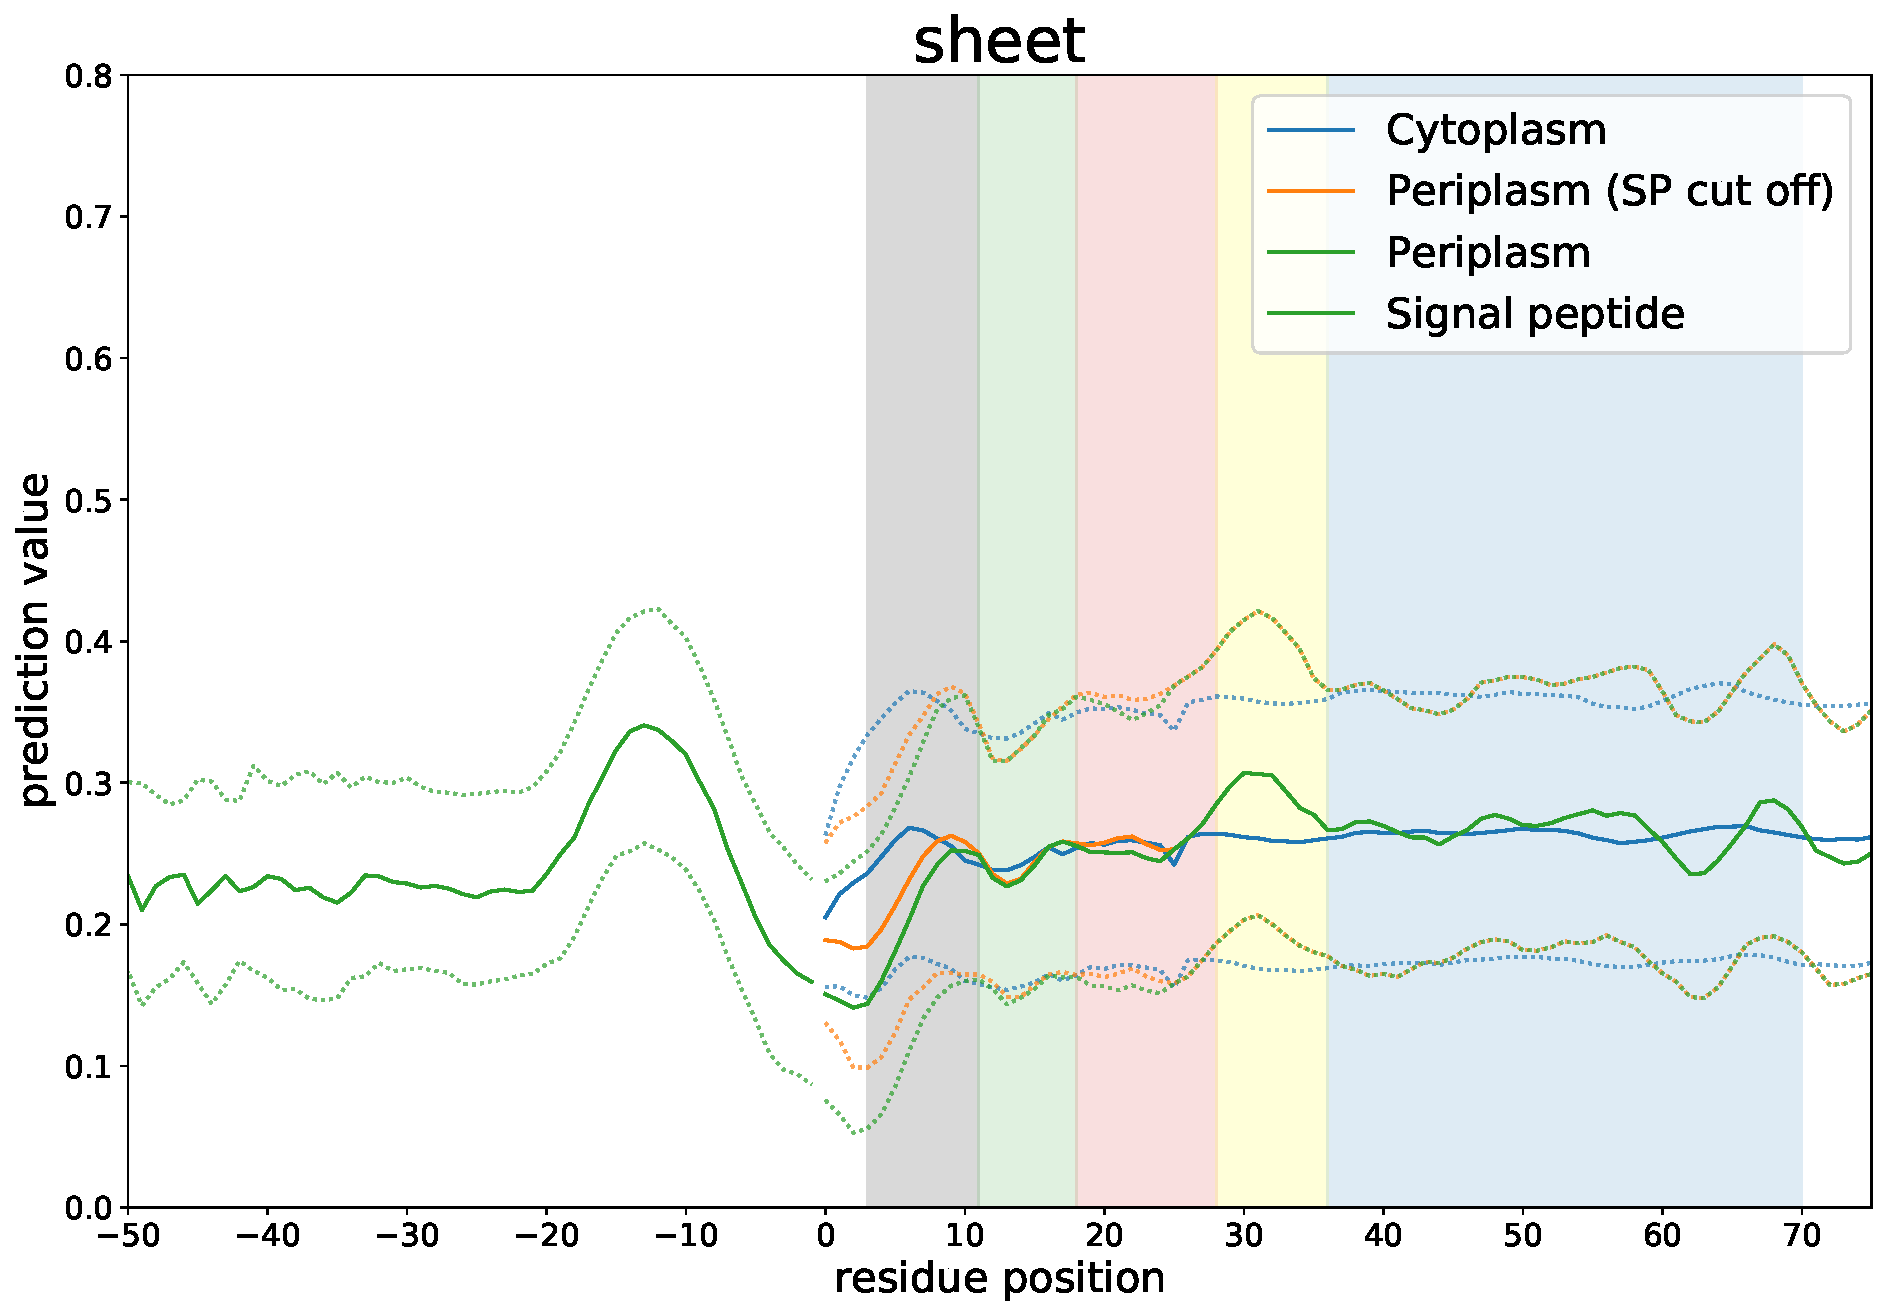
\includegraphics[width=\linewidth, height=0.46\textheight, keepaspectratio]{./results/general_comparison/local_comparison/img/local_sheet.pdf}
		\label{fig:local_sheet}
	~\end{subfigure}
~\end{figure}

~\begin{figure}[h!]
	\ContinuedFloat
	~\begin{subfigure}[b]{\linewidth}
		\centering
		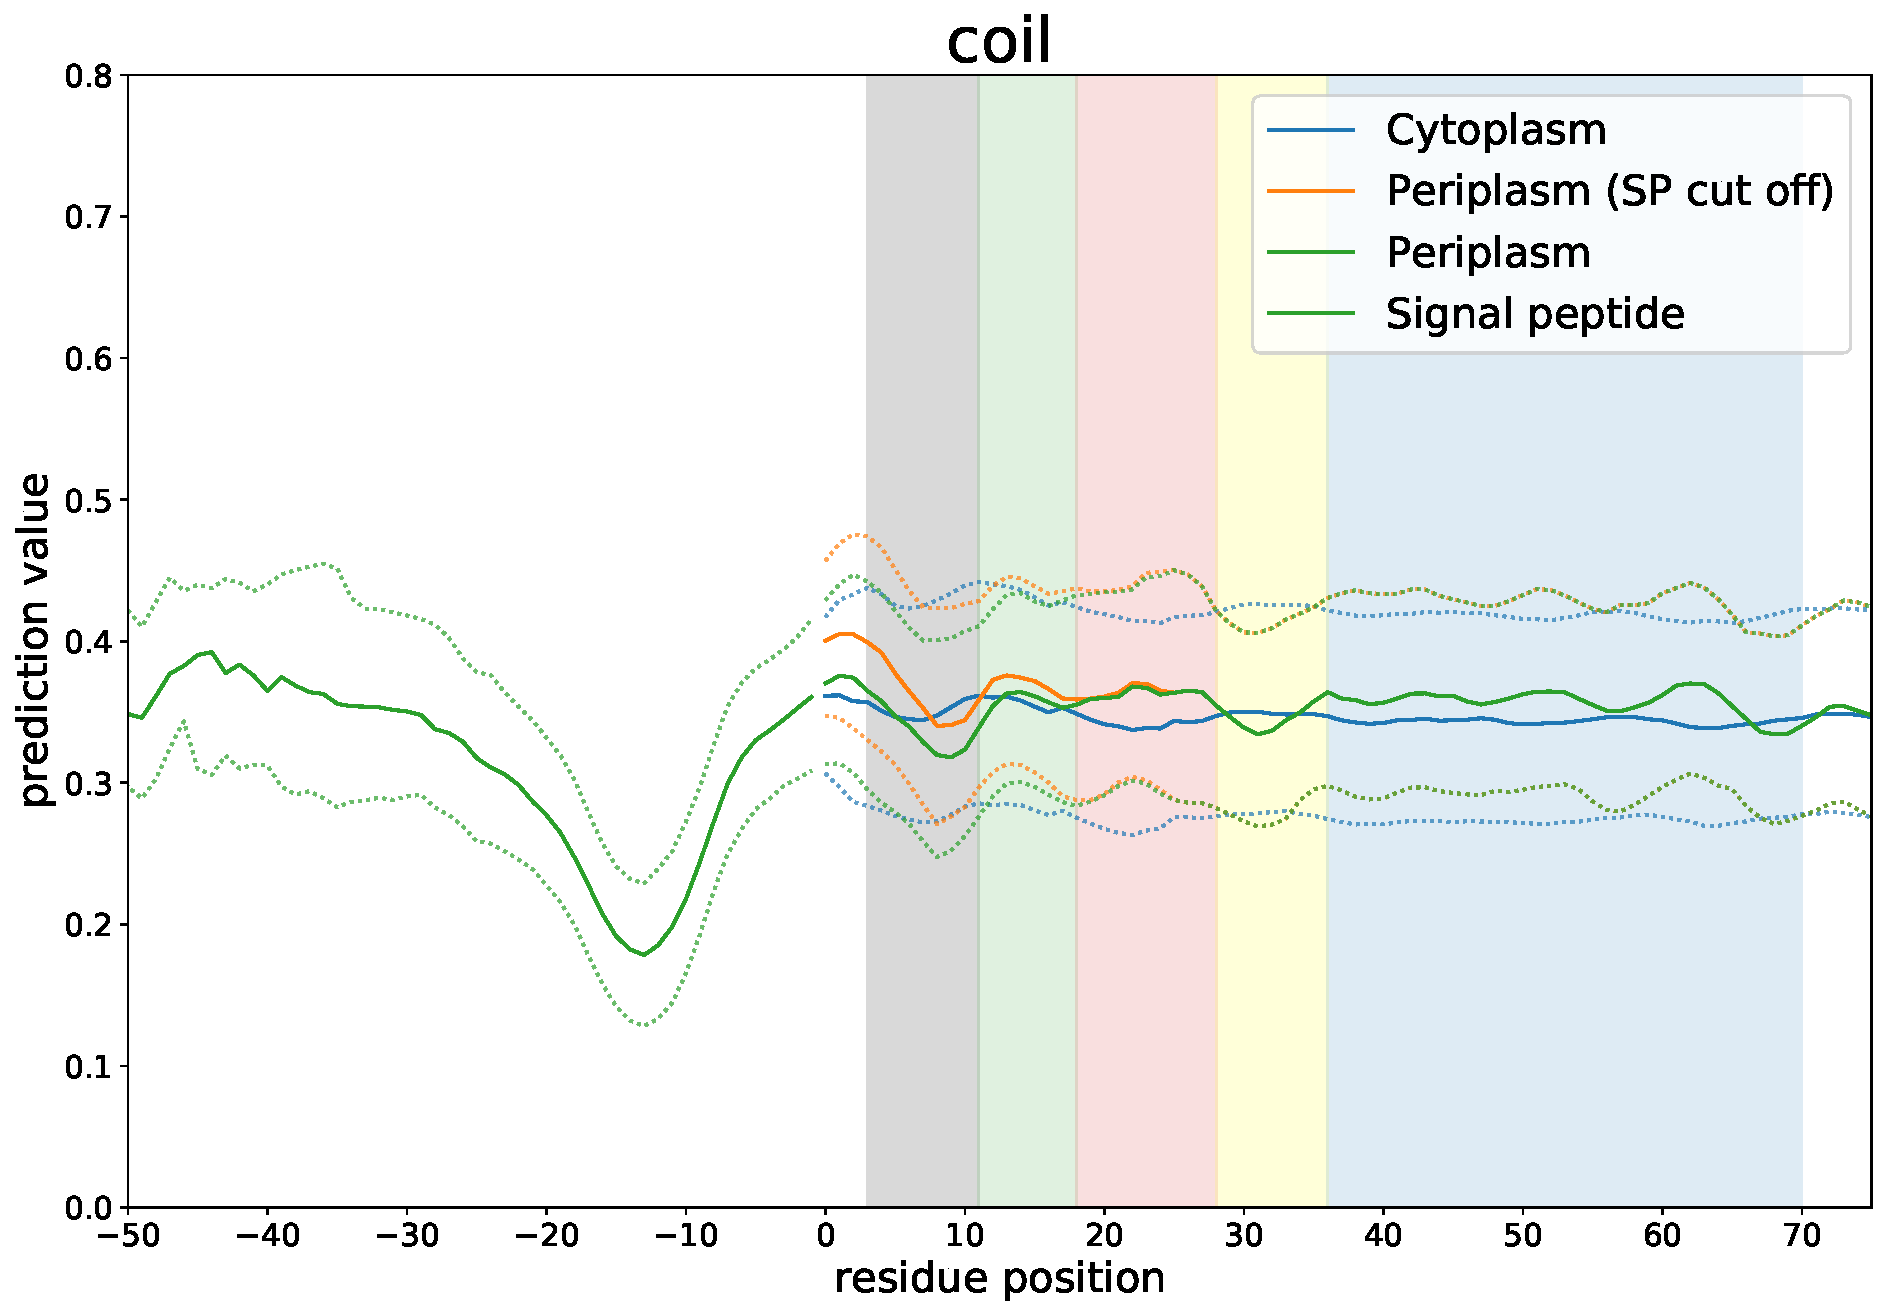
\includegraphics[width=\linewidth, height=0.46\textheight, keepaspectratio ]{./results/general_comparison/local_comparison/img/local_coil.pdf}
		\label{fig:local_coil}
	~\end{subfigure}
	\newline
	~\begin{subfigure}[b]{\linewidth}
		\centering
		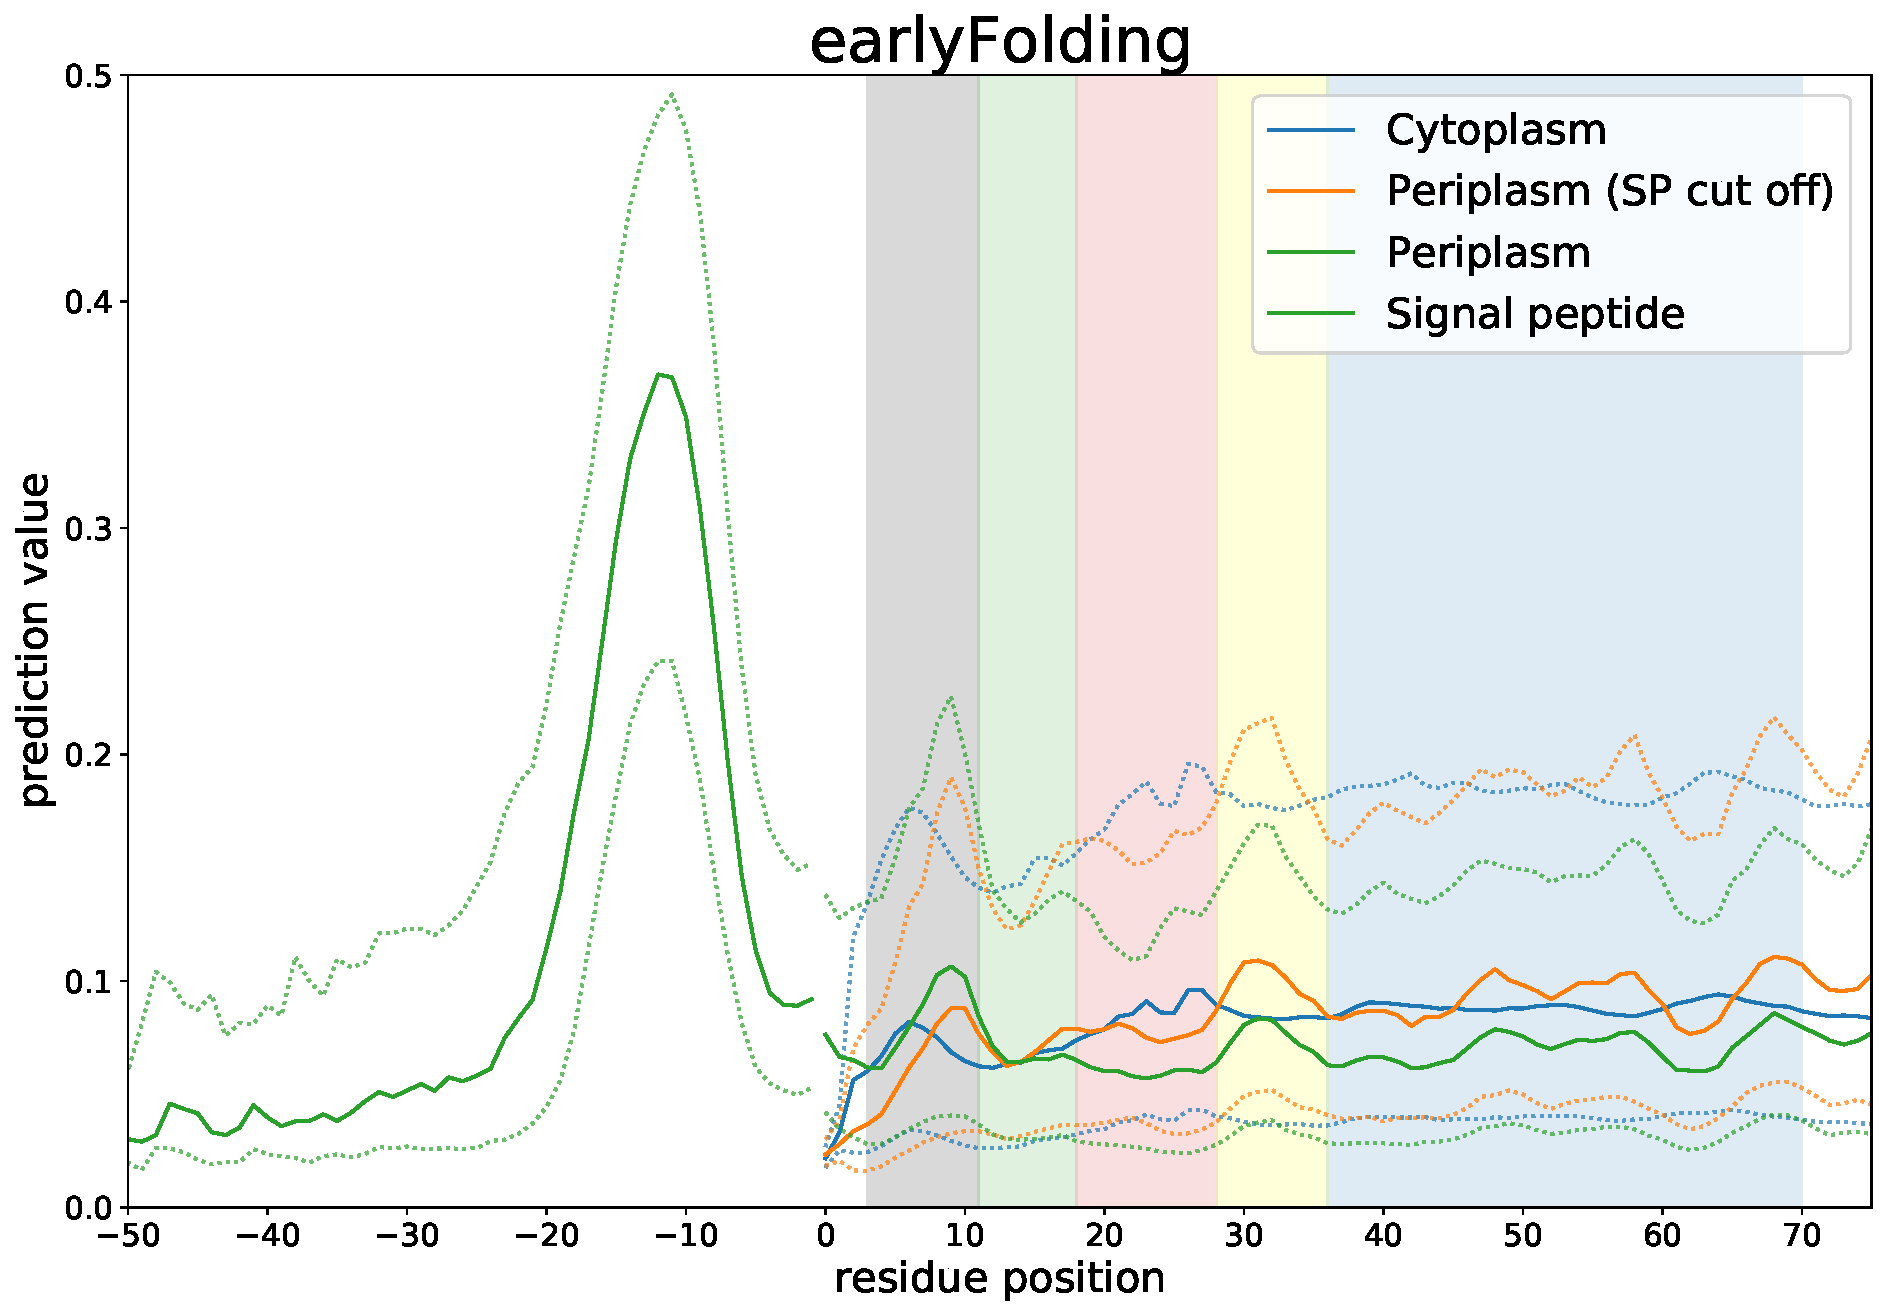
\includegraphics[width=\linewidth, height=0.46\textheight, keepaspectratio ]{./results/general_comparison/local_comparison/img/local_earlyFolding.pdf}
		\label{fig:local_earlyfolding}
	~\end{subfigure}
~\end{figure}


~\begin{figure}[h!]
	\ContinuedFloat
	~\begin{subfigure}[b]{\linewidth}
		\centering
		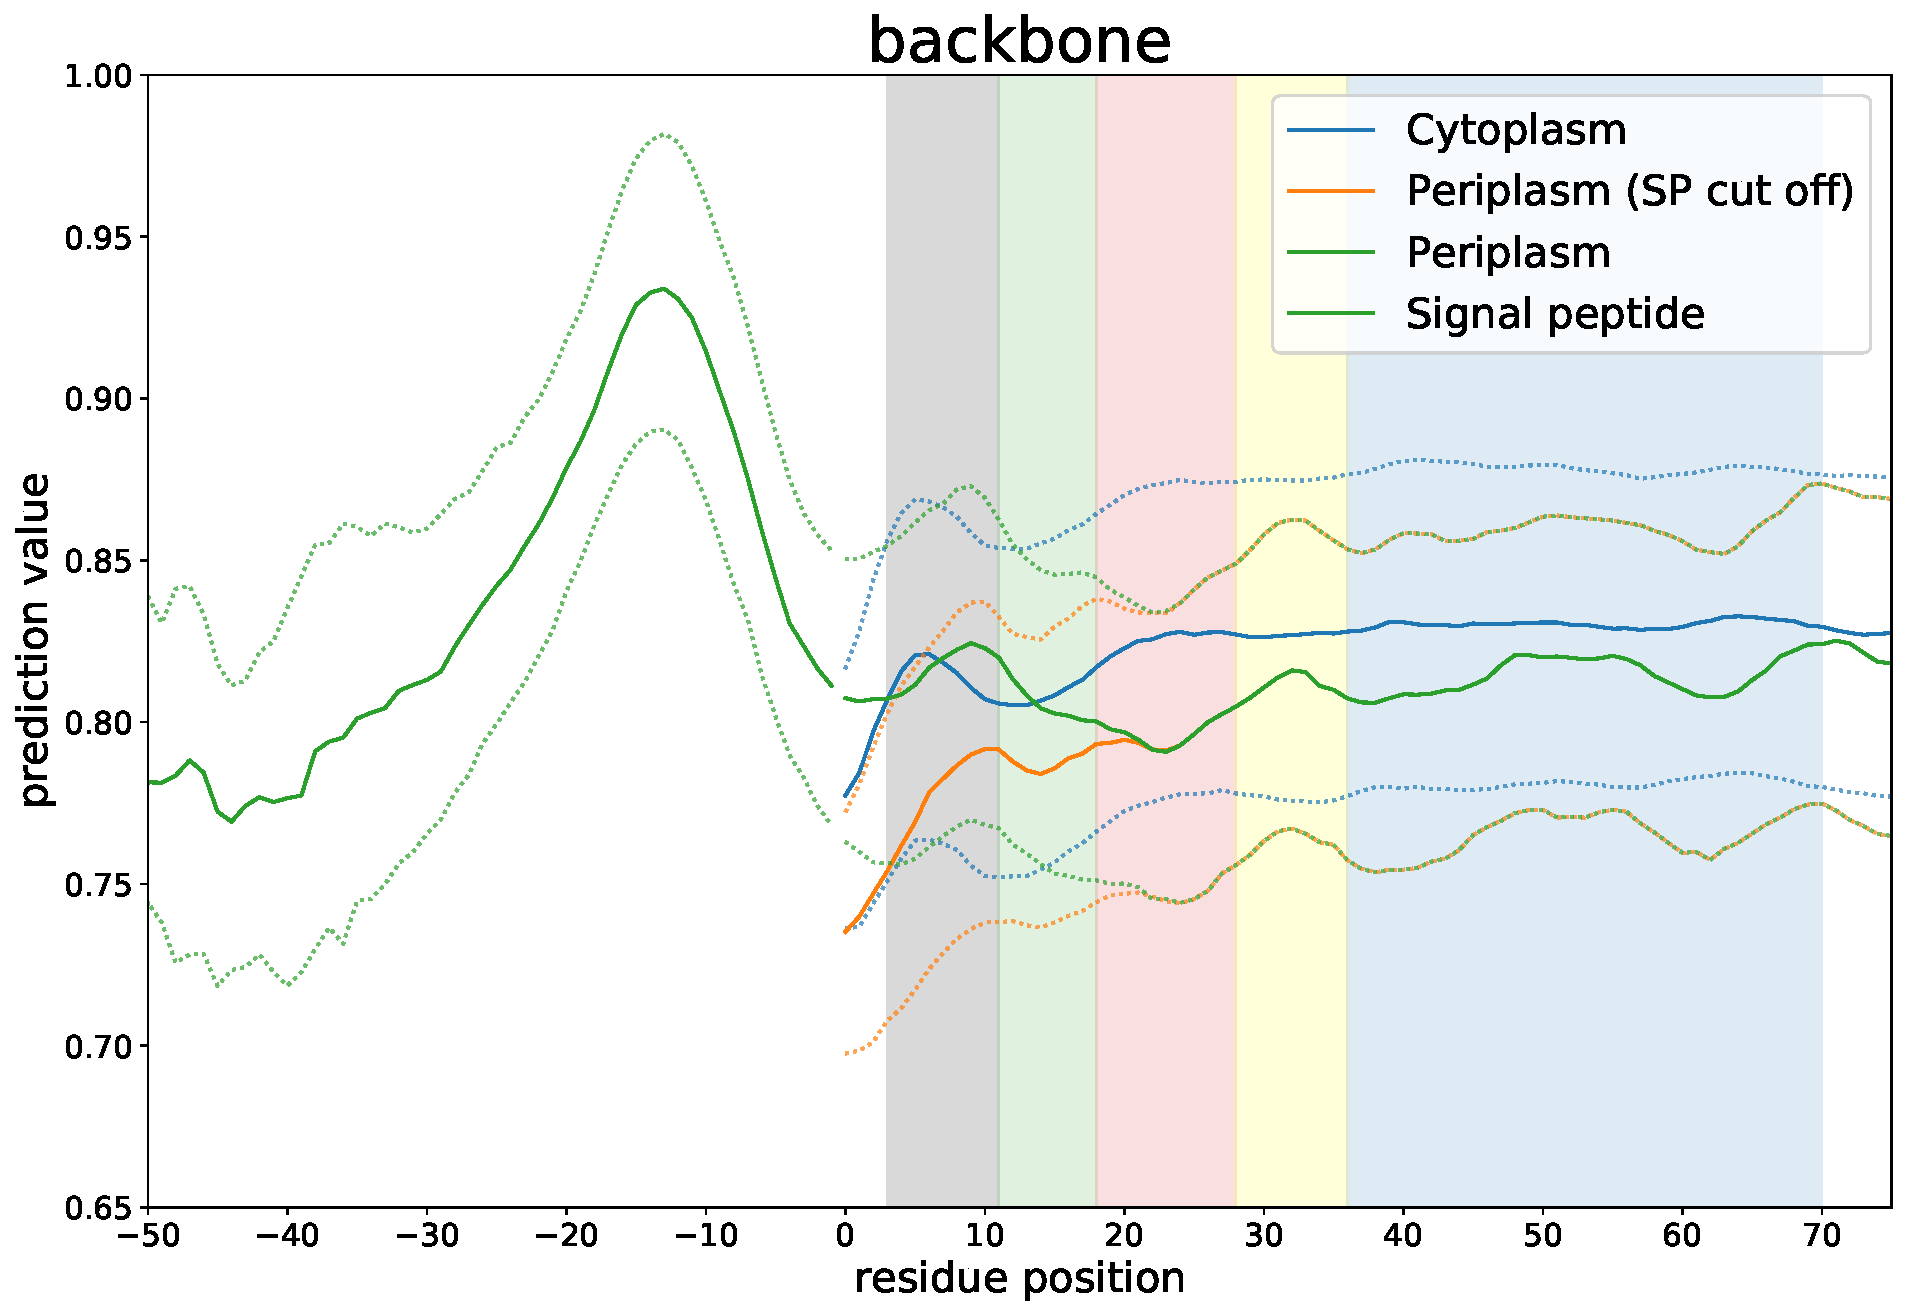
\includegraphics[width=\linewidth, height=0.37\textheight, keepaspectratio ]{./results/general_comparison/local_comparison/img/local_backbone.pdf}
		\label{fig:local_sheet}
	~\end{subfigure}
	\newline
	~\begin{subfigure}[b]{\linewidth}
		\centering
		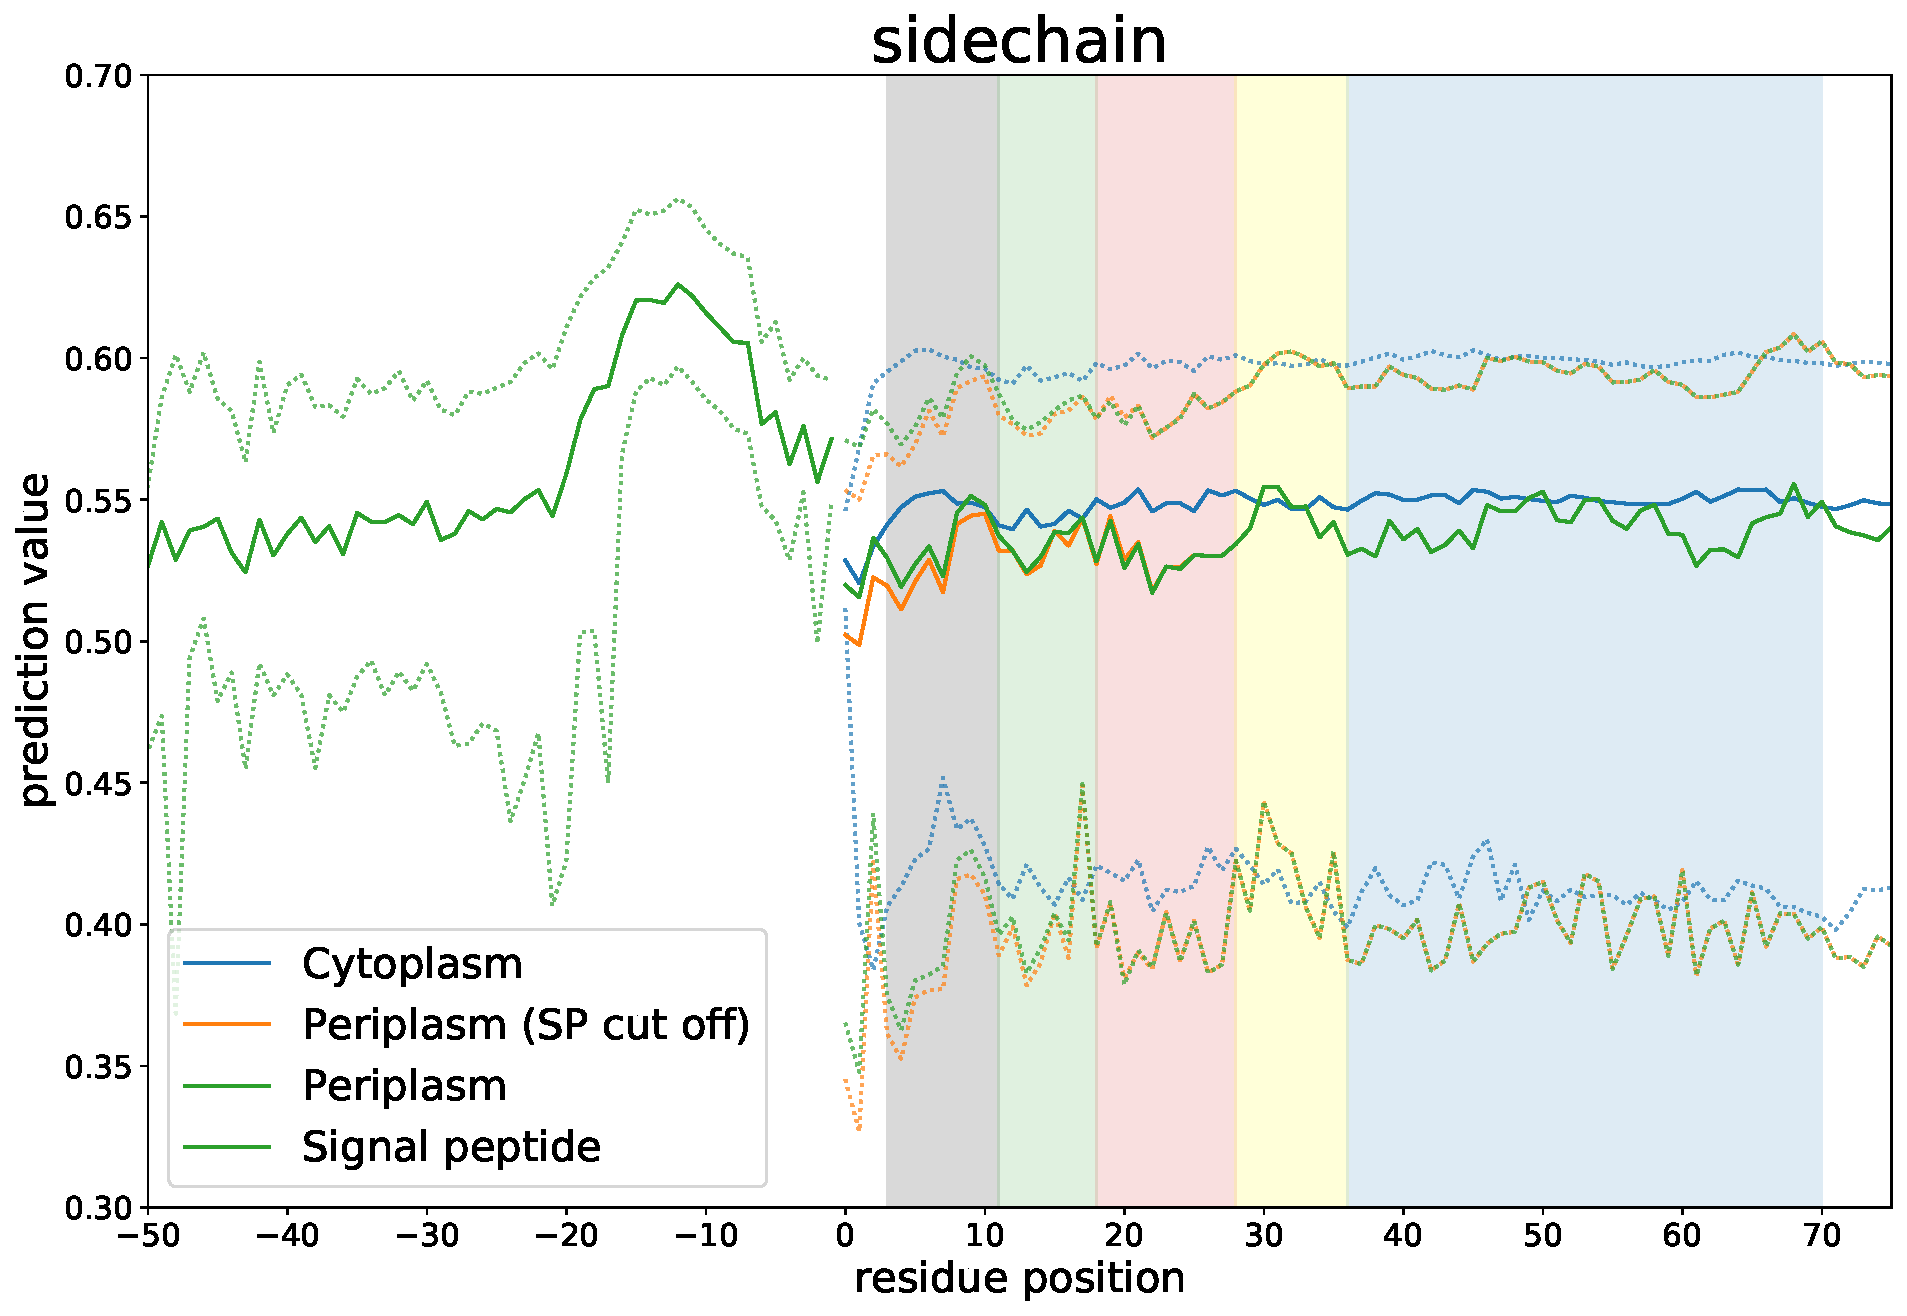
\includegraphics[width=\linewidth, height=0.37\textheight, keepaspectratio ]{./results/general_comparison/local_comparison/img/local_sidechain.pdf}
		\label{fig:local_coil}
	~\end{subfigure}
	\caption{
		\textbf{Propensity toward helix formation.}
		For each residue position, the median, first and third quartile were calculated.	
		Medians are shown by full colored lines,
		the quartiles by the dotted lines.
		Signal peptides are annotated with negative positions 
		so that the mature domains are aligned with the cytoplasmic protein.
		DynaMine only uses local sequence information to predict biophysical features.
		Therefore, the effect of the signal peptide is only observed on the graph until residue position 25.
		For later residue positions, the periplasm curve with signal peptide cut off (orange) and periplasm curve including the signal peptide (green) completely overlap.
		EFoldMine predictions (early folding) on the other hand can show distant effects on early folding of the signal peptide.
		\textbf{Signal Peptide}:residue -50 -- 0,
		\textbf{Grey region}:residue 3 -- 11,
		\textbf{Green region}:residue 11 -- 18,
		\textbf{Red region}:residue 18 -- 28,
		\textbf{Yellow region}:residue 28 -- 36,
		\textbf{Blue region}:residue 36 -- 70.
	}
	\label{fig:local_features}
~\end{figure}


			%\paragraph{Propensity towards helix formation}
			%	~\begin{comment}
Fig. \ref{fig:local_helix}) shows that cytoplasmic proteins have a higher propensity to form a helix at the beginning and near residue position 25 (as shown by the bump in the blue curve).
More C-terminal position do not show this preference as is depicted by the relatively even curve.
Mature periplasmic domains on the other hand seem to have a lower propensity toward helix formation as is observed starting from position 0 going to position 75.
The signal peptide itself displays a high tendency towards this secondary structure however, 
and this effect seems to be propagated to the N-terminal part of the periplasmic proteins.

Why cytoplasmic proteins have an increased tendency to form helices at near position 0 and 25,
while this is decreased in the mature domains of the periplasm remains unclear.
These same general regions seem to have a relative high propensity toward early folding both in cytoplasmic and periplasmic proteins and (Fig. \ref{fig:local_earlyfolding),
though in periplasmic proteins they are shifted toward the C-terminal end.
This could suggest that these regions play an important role in the folding process,
decreasing the propensity toward helix formation possible has a delaying effect.
~\end{comment}


			\paragraph{Signal Peptide}
				Fig.\ref{fig:local_features} (white regions) shows a clear signature of biophysical features for signal peptides.
In general, they have a higher propensity toward helix formation than toward the sheet or coil secondary structures.
However, for the most N-terminal part, the propensity towards forming a helix or forming a coil are very close to each other.
When reaching the region  close to position -20 (hydrophobic region), the propensity towards helix and sheet formation increases,
while the propensity towards coil formation decreases.

Within the C-region of the signal peptide, the propensity towards helix formation decreases again, 
but it is still the highest secondary structure propensity.
Generally, the C-terminal end of the signal peptides 
seems to have higher propensity to helix formation than the N-terminal end of the mature domain in periplasmic proteins.
Therefore, the signal peptide has positive effect towards forming a helix on the N-terminal end of the mature domain.
The C-region has a low propensity towards sheet formation,
and increasing propensity toward coil formation.
Also these tendencies propagates to the N-terminal part of the mature domain.  

In terms of dynamics, 
the H-region is the most rigid, both in backbone and sidechains.
In addition, it has high early folding propensity.
The C-region has a slight stabilizing effect on the sidechain dynamics of the N-terminal part of the mature domain,
and more significant stabilizing effect on the backbone dynamics.
The effect of the C-region on early folding propensity in the mature domain seems more complex.
While the N-terminal region of the mature domain increases in early folding propensity,
the rest of the protein seems to decrease.
One explanation for his behaviour is that the signal peptide can interact with the folding domains in the mature protein.
Because the signal peptide itself takes no part in the final protein,
all interactions with the signal peptide potentially delay the folding process.

In general, 
it seems that the signal peptides changes the secondary structure propensities, dynamical behaviour,
and early folding propensity of the N-terminal end of the mature domain.
These changed propensities increase the chance of forming interactions that are no part of the final fold,
thereby possible giving part of the mechanism behind the delayed folding observed in secreted proteins.

			\paragraph{Grey region}
				
In the grey region, or the first N-terminal 11 residues,
cytoplasmic and periplasmic proteins tend to have a region of relative high backbone rigidity (higher backbone propensity values) , 
surrounded by more flexible regions (N-terminal end and green region).
However, in periplasmic proteins, this rigidity is mainly due to the effect of the signal peptide 
as mature domains without signal peptide are predicted to have an increased backbone flexibility (lower backbone propensity values).
Sidechain dynamics has a higher propensity toward rigidity in the cytoplasmic proteins than those of the periplasm.
Both the cytoplasmic and periplasmic mature domains seem to have a similar propensity toward early folding,
but the presence of a signal peptide has a significant increasing effect.
Within the grey region,
cytoplasmic proteins have a higher tendency to form helices than periplasmic mature domains (without signal peptides),
but a lower propensity than periplasmic proteins that still have a signal peptide.
Sheet formation is similar for both groups,
with the presence of a signal peptide having the effect of lowering this propensity.
Finally, coil formation seems to be more frequent in periplasm mature domains than cytoplasmic proteins,
the presence of a signal peptide significantly decreases the propensity to form a coil.

			\paragraph{Green region}
				The green region goes from residue 11 to 18.
Most noticeably, this is the only region over the whole length of cytoplasmic proteins that shows increased backbone flexibility.
In all other regions, backbone dynamics is averaged out over the dataset of 30,632 cytoplasmic proteins.
This suggest that this flexible region is a general feature.
This region also exist in periplasmic proteins, 
but there it is shifted a little bit to the C-terminal end and extended into the red region.
Reduced early folding propensity is observed with similar values for all cytoplasmic an periplasic proteins.

			\paragraph{Red region}
				The red region spans from residue 18 to 28.
Most noticeably, starting in this region up to the end of the blue region (residue 70),
there is a clear difference in propensity to form helices in favor for cytoplasmic proteins.
Similarly, backbone and sidechain dynamics appear to be more rigid for cytoplasmic than periplasmic proteins.
There is a higher propensity toward early folding for cytoplasmic than periplasmic proteins in the red domain,
with the difference being more pronounced when including the effect of signal peptides.
It is interesting to see that cytoplasmic proteins seem to have a general preference for helix formation in this region,
As in other parts of the protein, there seems to be more of a constant background preference as a result of averaging out over many proteins.
Combining this observation with previous one suggests that cytoplasmic proteins prefer on average a flexible region followed by an helix near the N-terminus.
Another possibility is that they prefer either an helix or a flexible region.
It is not possible to distinguish between these hypothesises with this analysis.

			\paragraph{Yellow region}
				In the yellow region (residue 28 to 36),
a sudden spike in propensity propensity towards sheet formation and early folding is observed in periplasmic proteins,
but not in cytoplasmic ones.
There is also an positive effect on backbone and sidechain rigidity,
and a negative effect on coil formation.
This behaviour seems to be very specific to periplasmic proteins,
occurring with a high enough frequency not to be averaged out over the 3,883 proteins.
The reason for the presence of this increased propensity towards sheet formation accompanied by early folding propensity remains unclear however, 
but could be an interesting subject for further research.



			\paragraph{Blue region}
				The blue region shows an increased propensity toward coil formation in periplasmic proteins as compared to cytoplasmic proteins.
Additionally, periplasmic proteins are more flexible in backbone and sidechain and less prone to form a helix.

			\paragraph{Final remarks}
				It should be noted that comparing periplasmic to cytoplasmic protein on a large scale comes with its own set of advantages and limitations.
As the cytoplasmic dataset contained about 10 times more protein sequences than the periplasmic dataset,
the cytoplasmic curves are to be expected to appear flatter and smoother than the periplasmic curves.
As this analysis looked at variation in function of position,
only position specific tendencies can be observed.
This way it was observed that cytoplasmic proteins seemed to form a preference toward helix formation in the red region,
periplasmic proteins have an increased preference to form sheets in the yellow region,
and a general region of rigidity and early folding propensity followed by an relative flexible region of decreased early folding propensity near the beginning of a protein for both cytoplasmic and periplasmic proteins.
In periplasmic proteins, this flexible regions seems to be more extensive.
Only features that occur in a relative large part of the proteins will be revealed by this analysis,
which should make them more robust, but it has the downside that other features remain obscured.
However it is striking that even with this many proteins,
tendencies are observed without being averaged out.
Exact positions associated with the different regions should not be taken to strictly.
For example, the increased propensity towards helix formation observed at position 25  
would still be observed even if in reality this helix occurs more in distribution around position 25,
possibly with a quite high deviation.
It is also impossible to conclude from this analysis which tendencies occur together, which can but don't have to occur together and which are mutually exclusive.
Finally, 
features that rely more on a relative position to another feature rather than an absolute position will not be clarified by this analysis.

				
	\subsection{Comparison of the biophysical landscape between twins}
		
		In previous section the biophysical features of cytoplasmic and periplasmic proteins were compared both globally and in function of residue position.
In this section, the difference of characteristics will be examined in more detail.
To achieve this, the UniProtKB databank was searched for structural twins,
homologues for which one sequence resides in the cytoplasm and one the periplasm.
The advantage of this approach is that structural twins have a very similar biophysical landscape,
making differences more likely to be related to the final protein location.

		%\subsubsection{Large scale cytoplasmic/periplasmic twin search}
		%	The twin dataset (see methods) is given in Table. \ref{table:twins}.

~\begin{longtable}[]{@{}lllllll@{}}
\toprule
& Cytoplasm uniref50 & cluster size & Periplasm uniref50 & cluster size \tabularnewline
\midrule
\endhead
0 & UniRef50\_Q2NVU4 & 124 & UniRef50\_A0A1X1D1X1 & 148 \tabularnewline
1 & UniRef50\_P83221 & 4189 & UniRef50\_O53021 & 2118 \tabularnewline
2 & UniRef50\_Q96VT4 & 1678 & UniRef50\_O59651 & 9906 \tabularnewline
3 & UniRef50\_P0A963 & 3836 & UniRef50\_P00805 & 2537 \tabularnewline
4 & UniRef50\_P0AAL2 & 1270 & UniRef50\_P0AAL4 & 492 \tabularnewline
5 & UniRef50\_P10902 & 6730 & UniRef50\_P0C278 & 160 \tabularnewline
6 & UniRef50\_P21517 & 4496 & UniRef50\_P25718 & 5447 \tabularnewline
7 & UniRef50\_O33732 & 29 & UniRef50\_P39185 & 6749 \tabularnewline
8 & UniRef50\_P44650 & 243 & UniRef50\_P44652 & 304 \tabularnewline
9 & UniRef50\_P0A9L3 & 1427 & UniRef50\_P45523 & 2225 \tabularnewline
10 & UniRef50\_P12994 & 1160 & UniRef50\_P77368 & 1614 \tabularnewline
11 & UniRef50\_Q8ZRT8 & 1014 & UniRef50\_Q32JZ5 & 878 \tabularnewline
12 & UniRef50\_Q72CB8 & 24 & UniRef50\_Q72EC8 & 17 \tabularnewline
13 & UniRef50\_A0A432R1Z2 & 206 & UniRef50\_Q7M827 & 379 \tabularnewline
14 & UniRef50\_P62602 & 2175 & UniRef50\_Q8XDH7 & 3943 \tabularnewline
15 & UniRef50\_Q32JZ5 & 878 & UniRef50\_Q8ZRT8 & 1014 \tabularnewline
\bottomrule
\caption{\textbf{Twins of UniRef50 clusters.}
Table shows twins of UniRef50 clusters with cluster size next to it.
Each twin of clusters contains at least one pair of twin proteins within the same organism.}
\label{table:twins}
~\end{longtable}


		\subsubsection{Biophysical feature comparison between twins}
			
As was shown in previous analysis,
signal peptides tend to promote helix formation and demote coil formation near the N-terminal end of the protein (Fig. \ref{fig:twin_helix}, \ref{fig:twin_coil}).
Little effect was seen on the propensity toward sheet formation (Fig. \ref{fig:twin_sheet}).
In addition, the signal peptide seems to have a stabilizing effect on backbone dynamics near the N-terminal end (Fig. \ref{fig:twin_backbone}).
Overall, there seems to be a higher propensity toward helix formation and backbone rigidity in cytoplasmic than periplasmic proteins.
Interestingly, previous analysis showed that periplasmic proteins have a higher tendency toward coil formation from residue 20 to 70 (red,yellow and blue region), with dip near residue 33 (yellow region).
This also shows in the twin analysis (Fig. \ref{fig:twin_coil}),
were there seems to be an slight preference for coil formation in periplasmic proteins, 
except for region near residue 33 where there is clear decrease in preference.
In the previous analysis this yellow regions near residue 33 showed a clear peak in propensity toward sheet formation for periplasmic proteins.
This is not observed in the twin analysis, 
instead periplasmic proteins display an increased preference for helix formation.
At the same position, an increased preference for early folding is observed in periplasmic proteins,
as well as increased sidechain rigidity.
This suggests that the region near position 33 plays an important role in translocation toward the periplasm,
as it folds earlier with an decreased preference to form a coil.

~\begin{figure}[h!]
	~\begin{subfigure}[b]{\linewidth}
			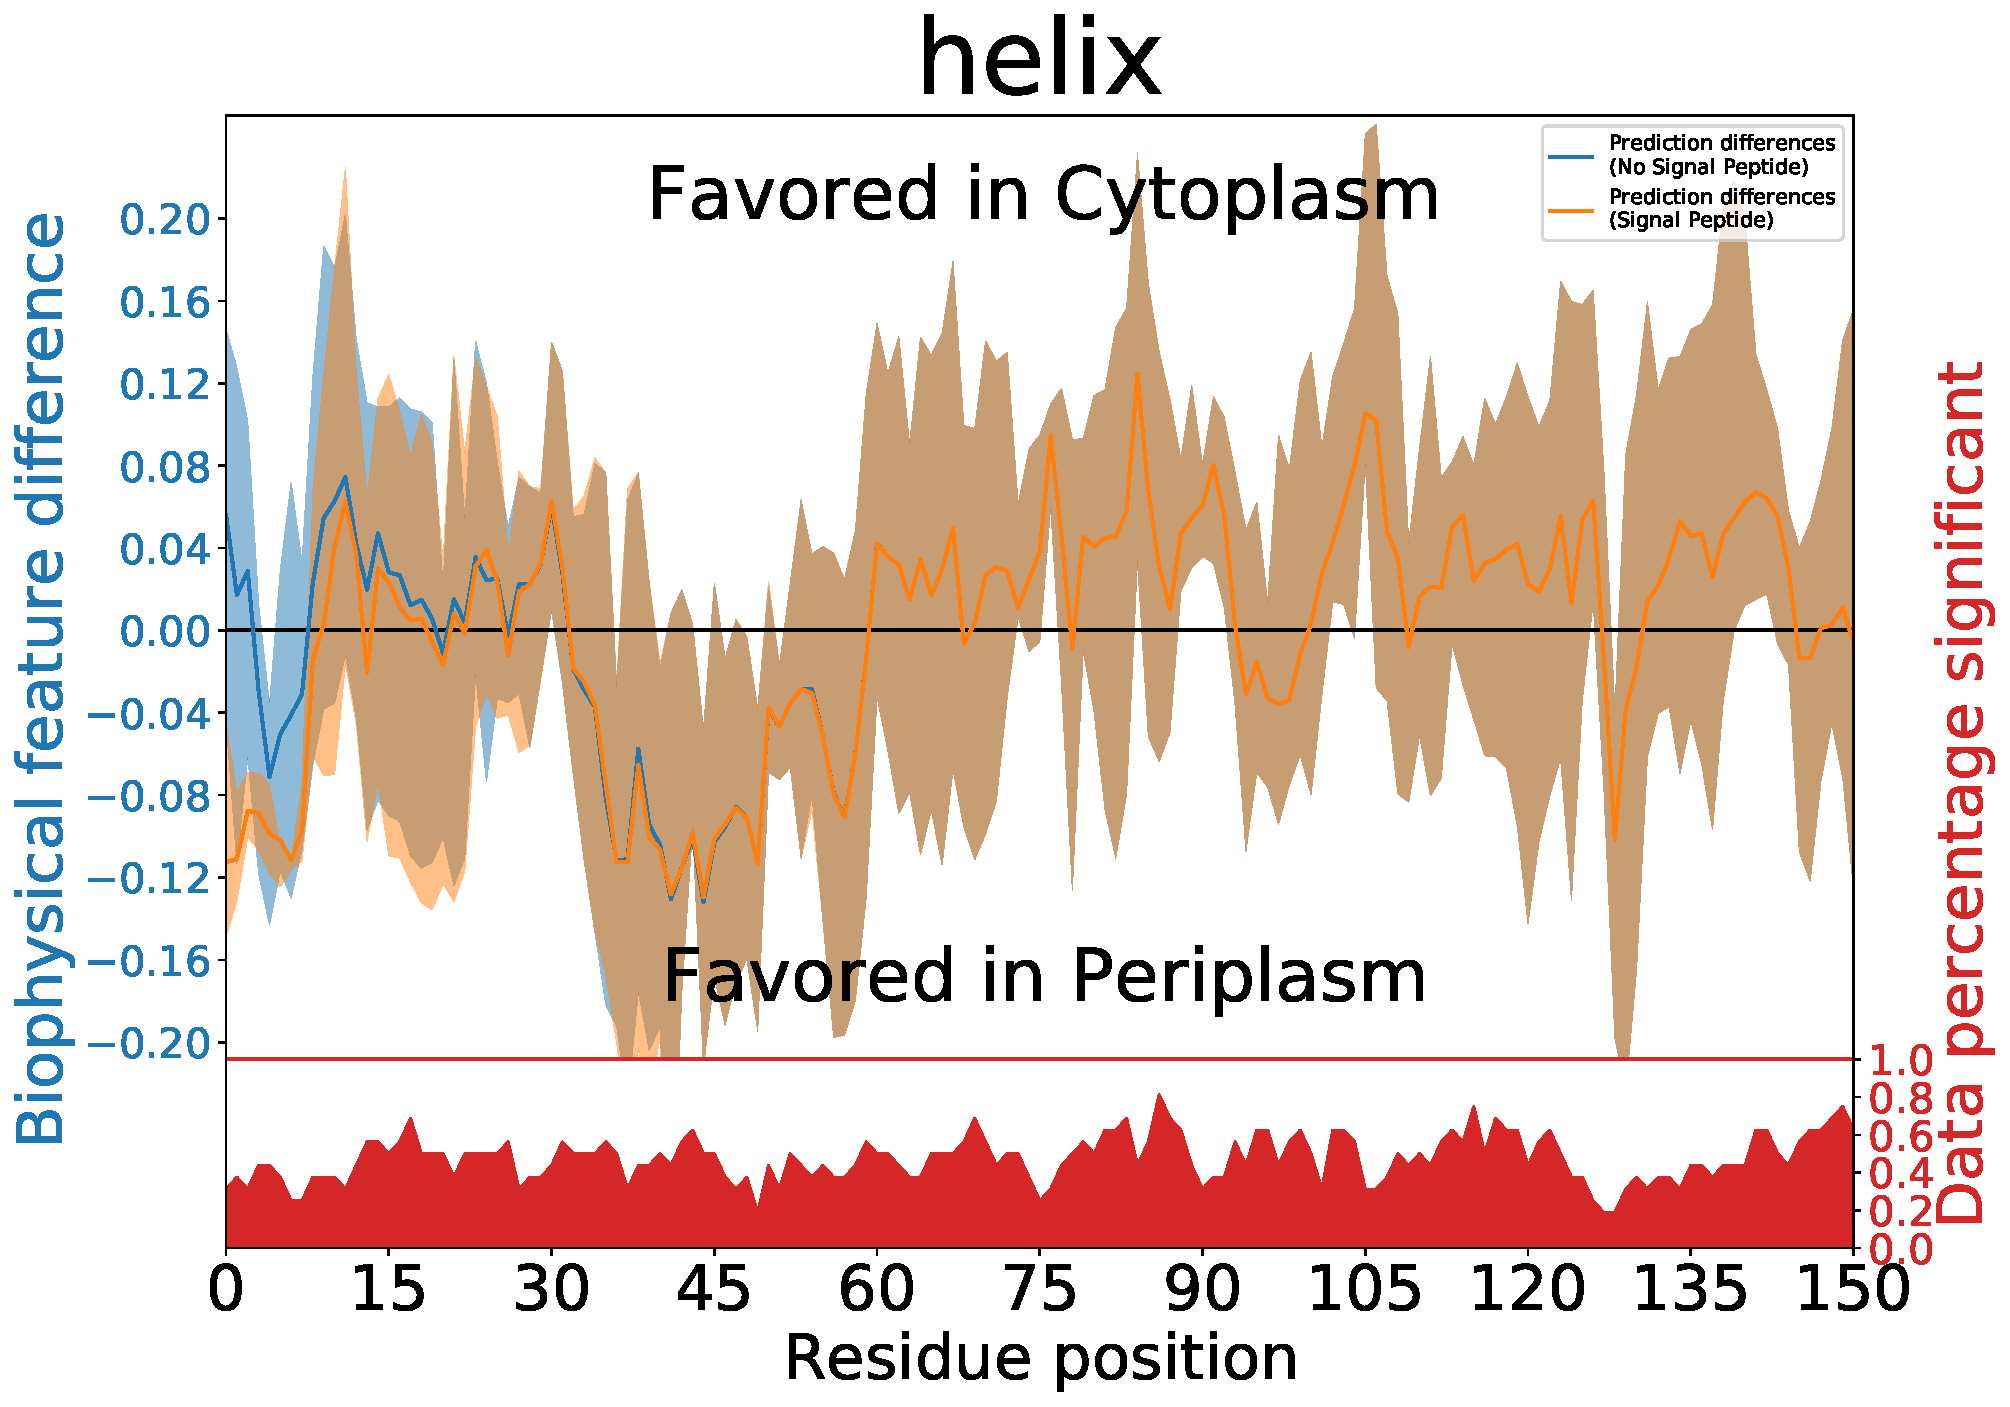
\includegraphics[width=\linewidth, height=0.43\textheight, keepaspectratio]
	{./results/twins/img/helix.pdf}
		\caption{}
		\label{fig:twin_helix}
	~\end{subfigure}
	\newline
	~\begin{subfigure}[b]{\linewidth}
			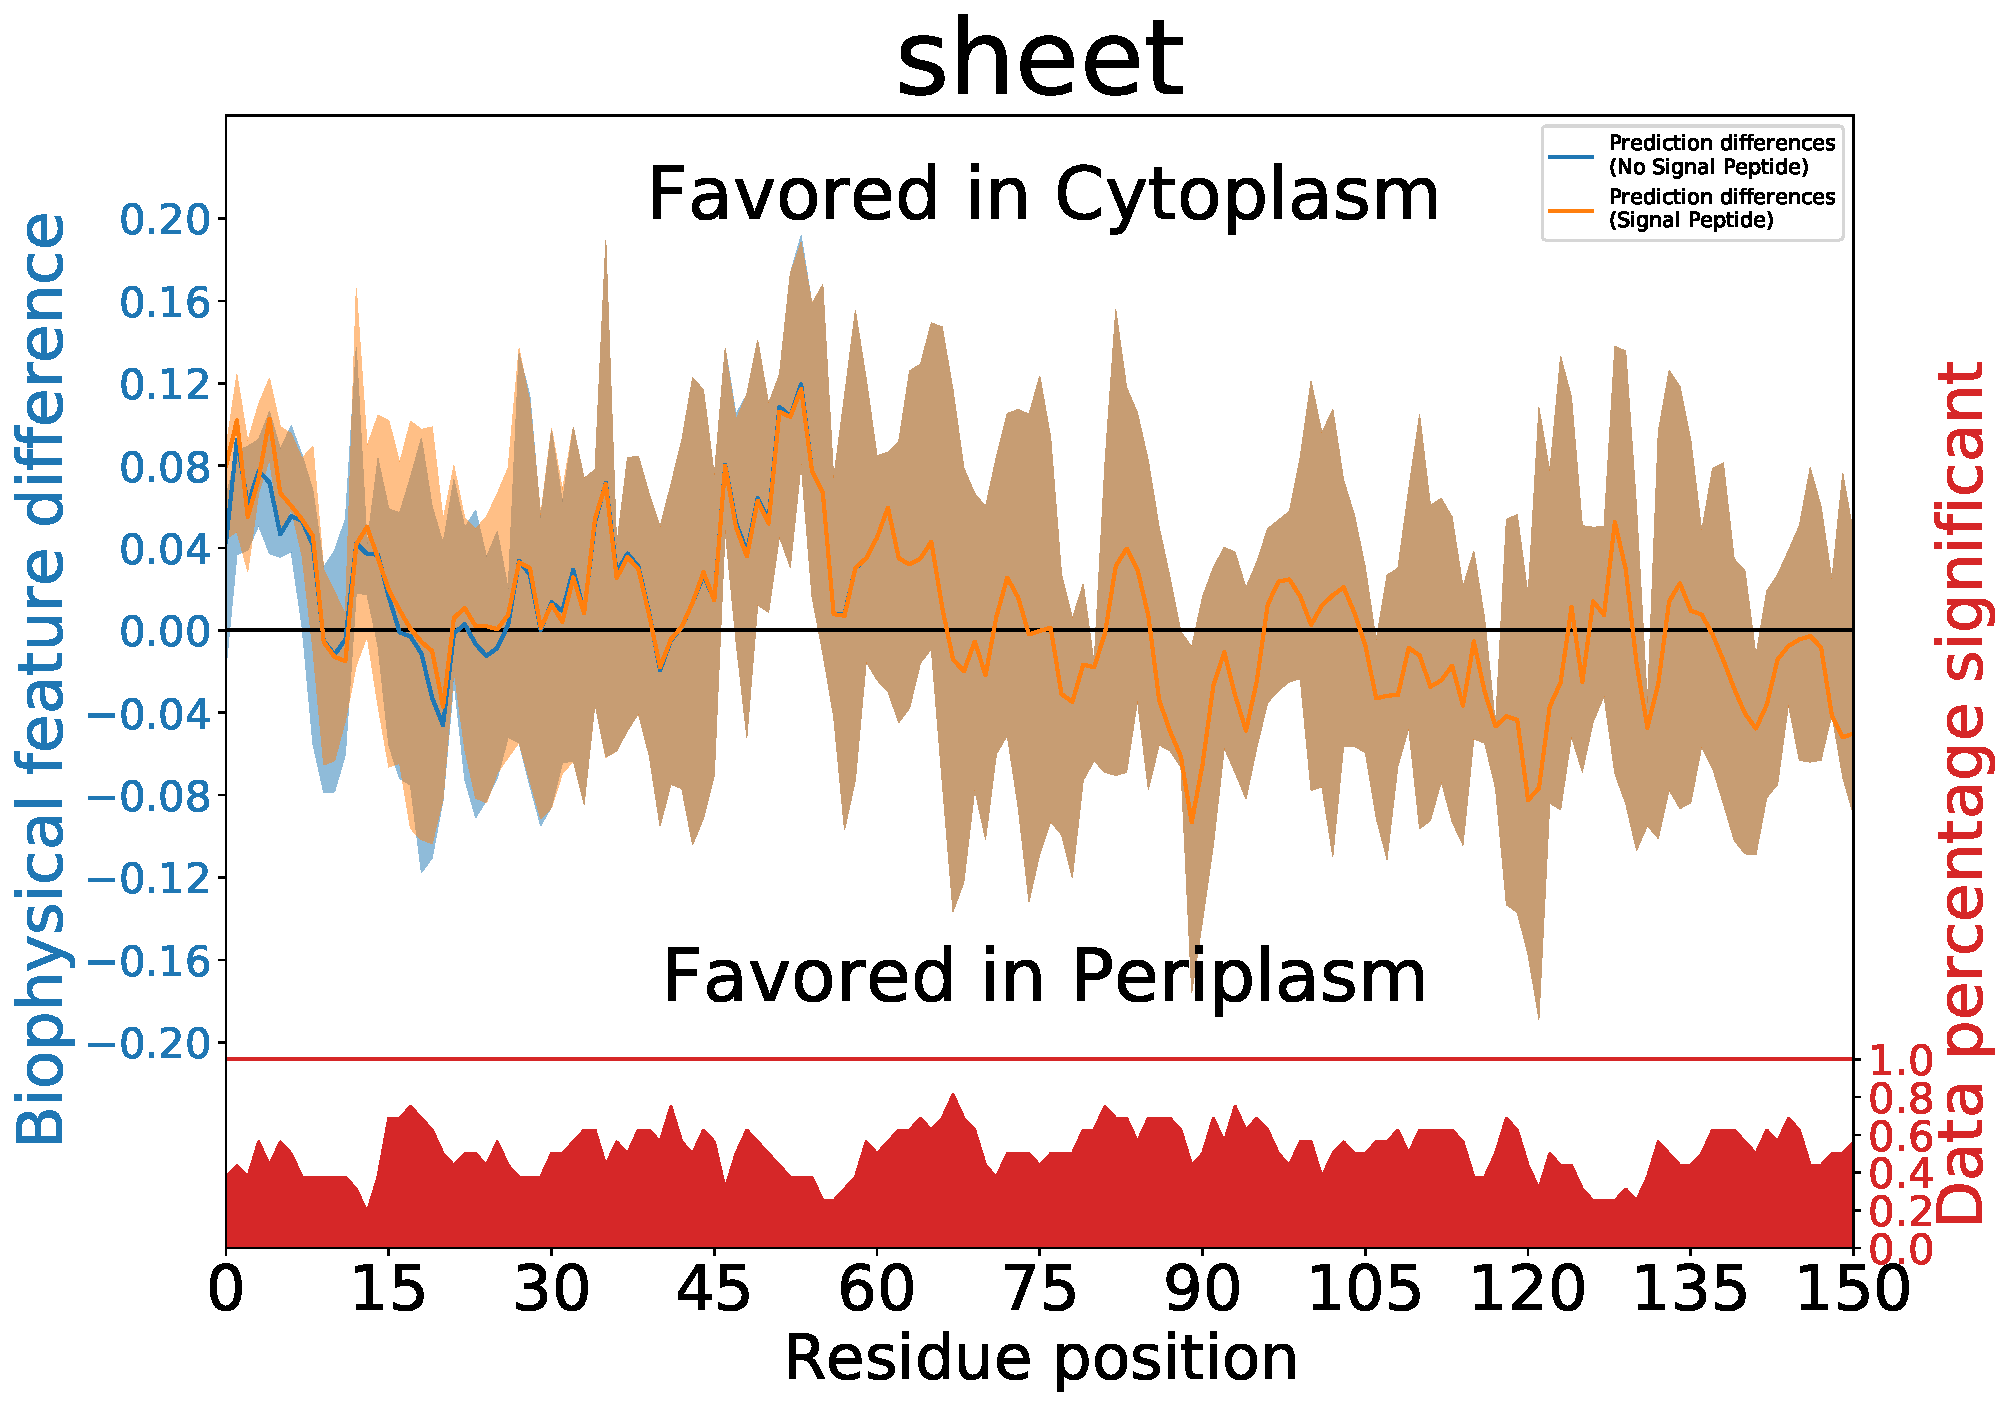
\includegraphics[width=\linewidth, height=0.43\textheight, keepaspectratio]
	{./results/twins/img/sheet.pdf}
		\caption{}
		\label{fig:twin_sheet}
	~\end{subfigure}
~\end{figure}


~\begin{figure}[h!]
	\ContinuedFloat
	~\begin{subfigure}[b]{\linewidth}
		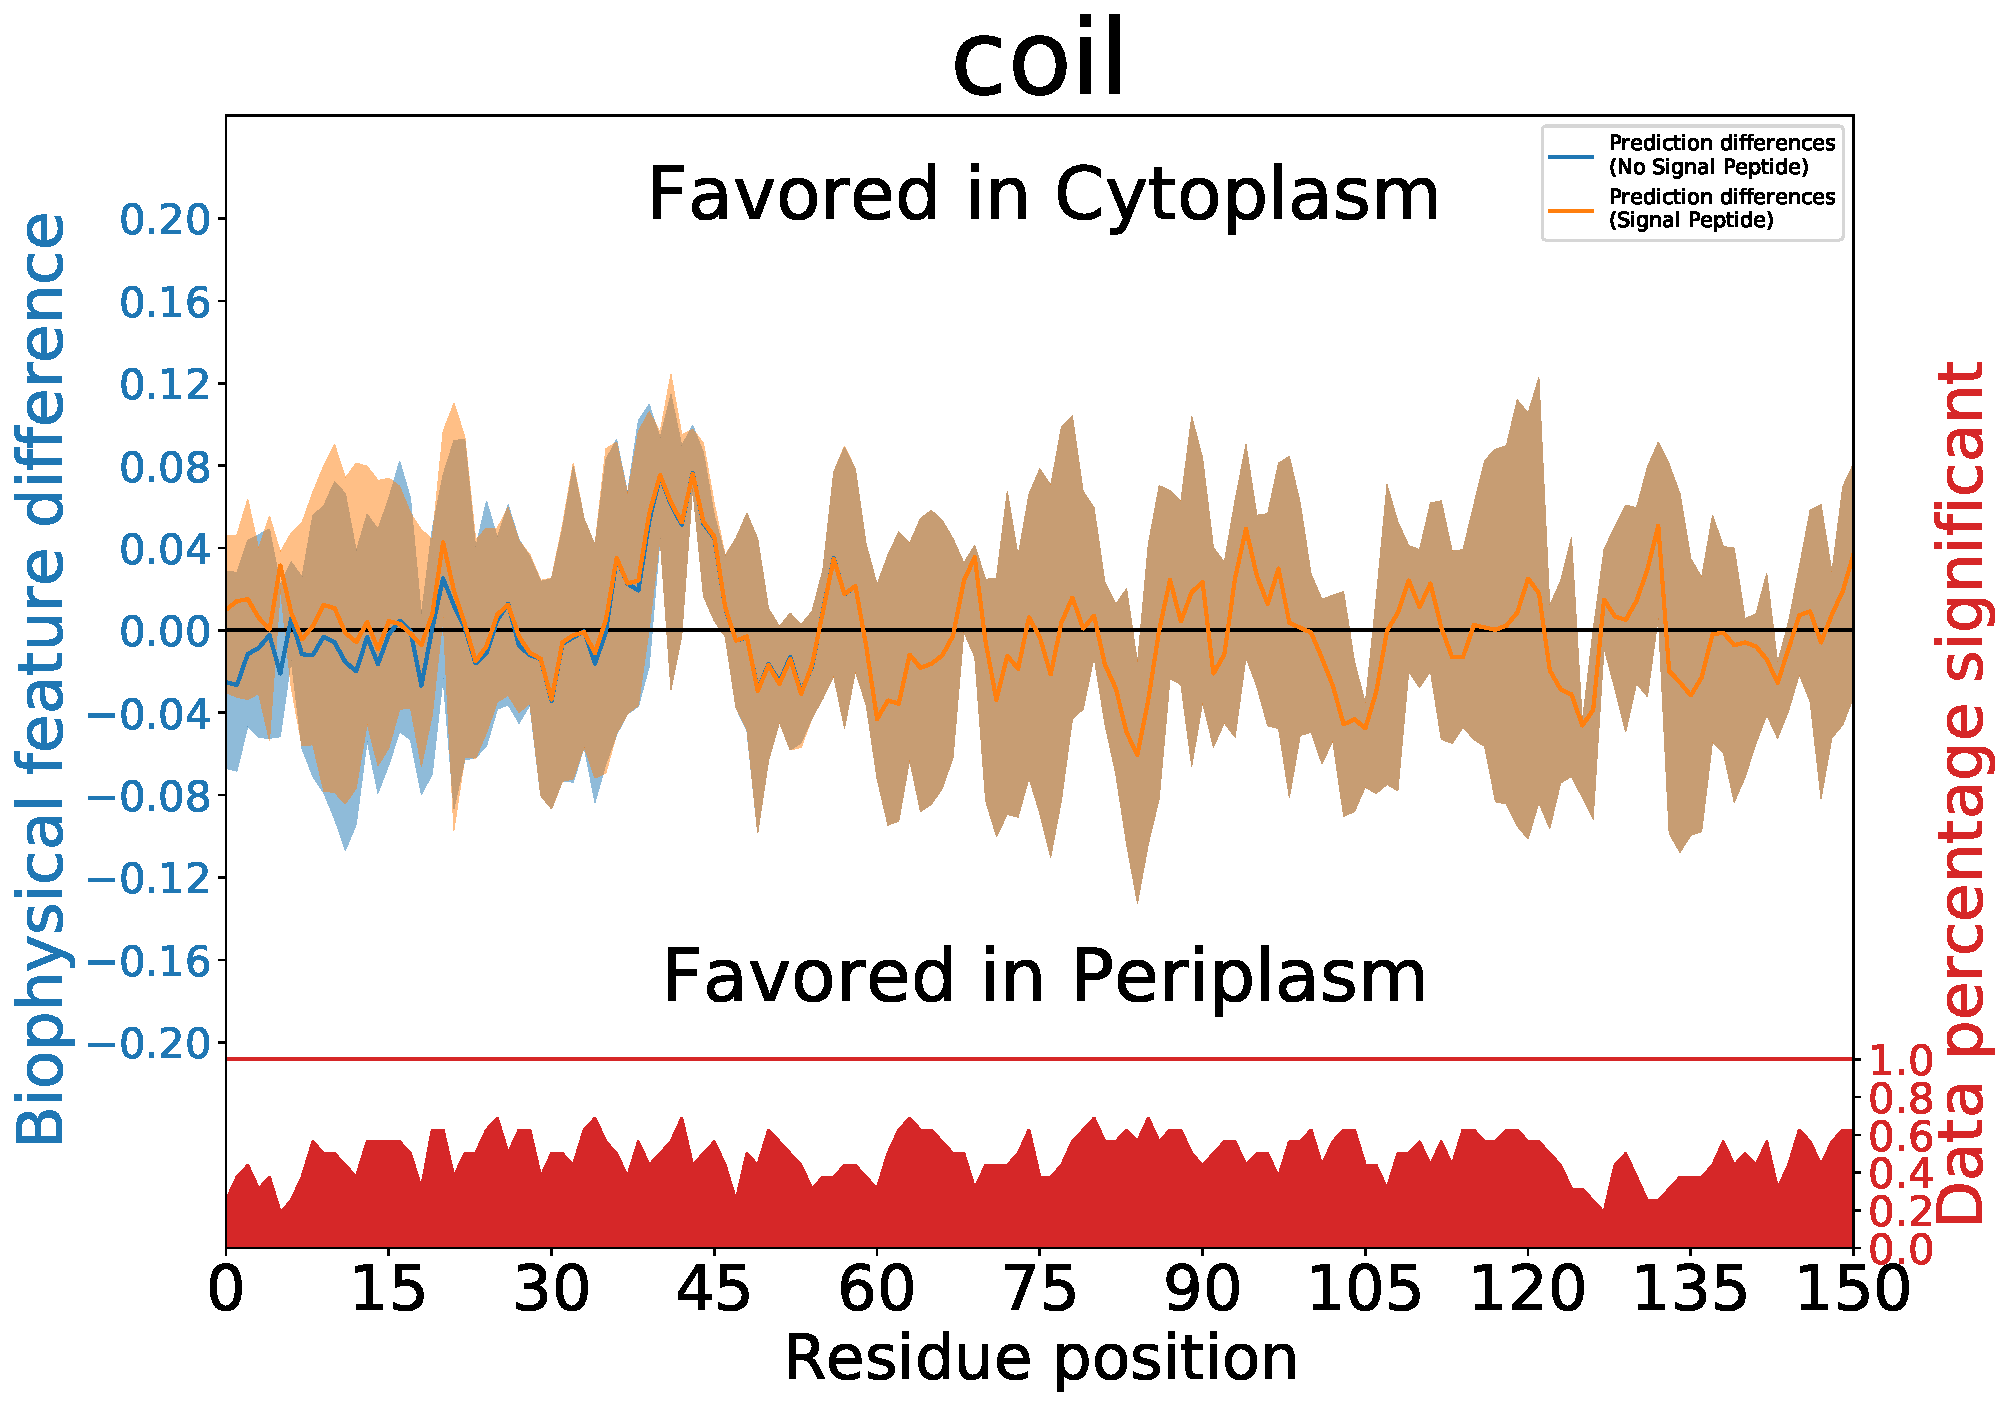
\includegraphics[width=\linewidth, height=0.43\textheight, keepaspectratio]
	{./results/twins/img/coil.pdf}
		\caption{}
		\label{fig:twin_coil}
	~\end{subfigure}
	\newline
	~\begin{subfigure}[b]{\linewidth}
			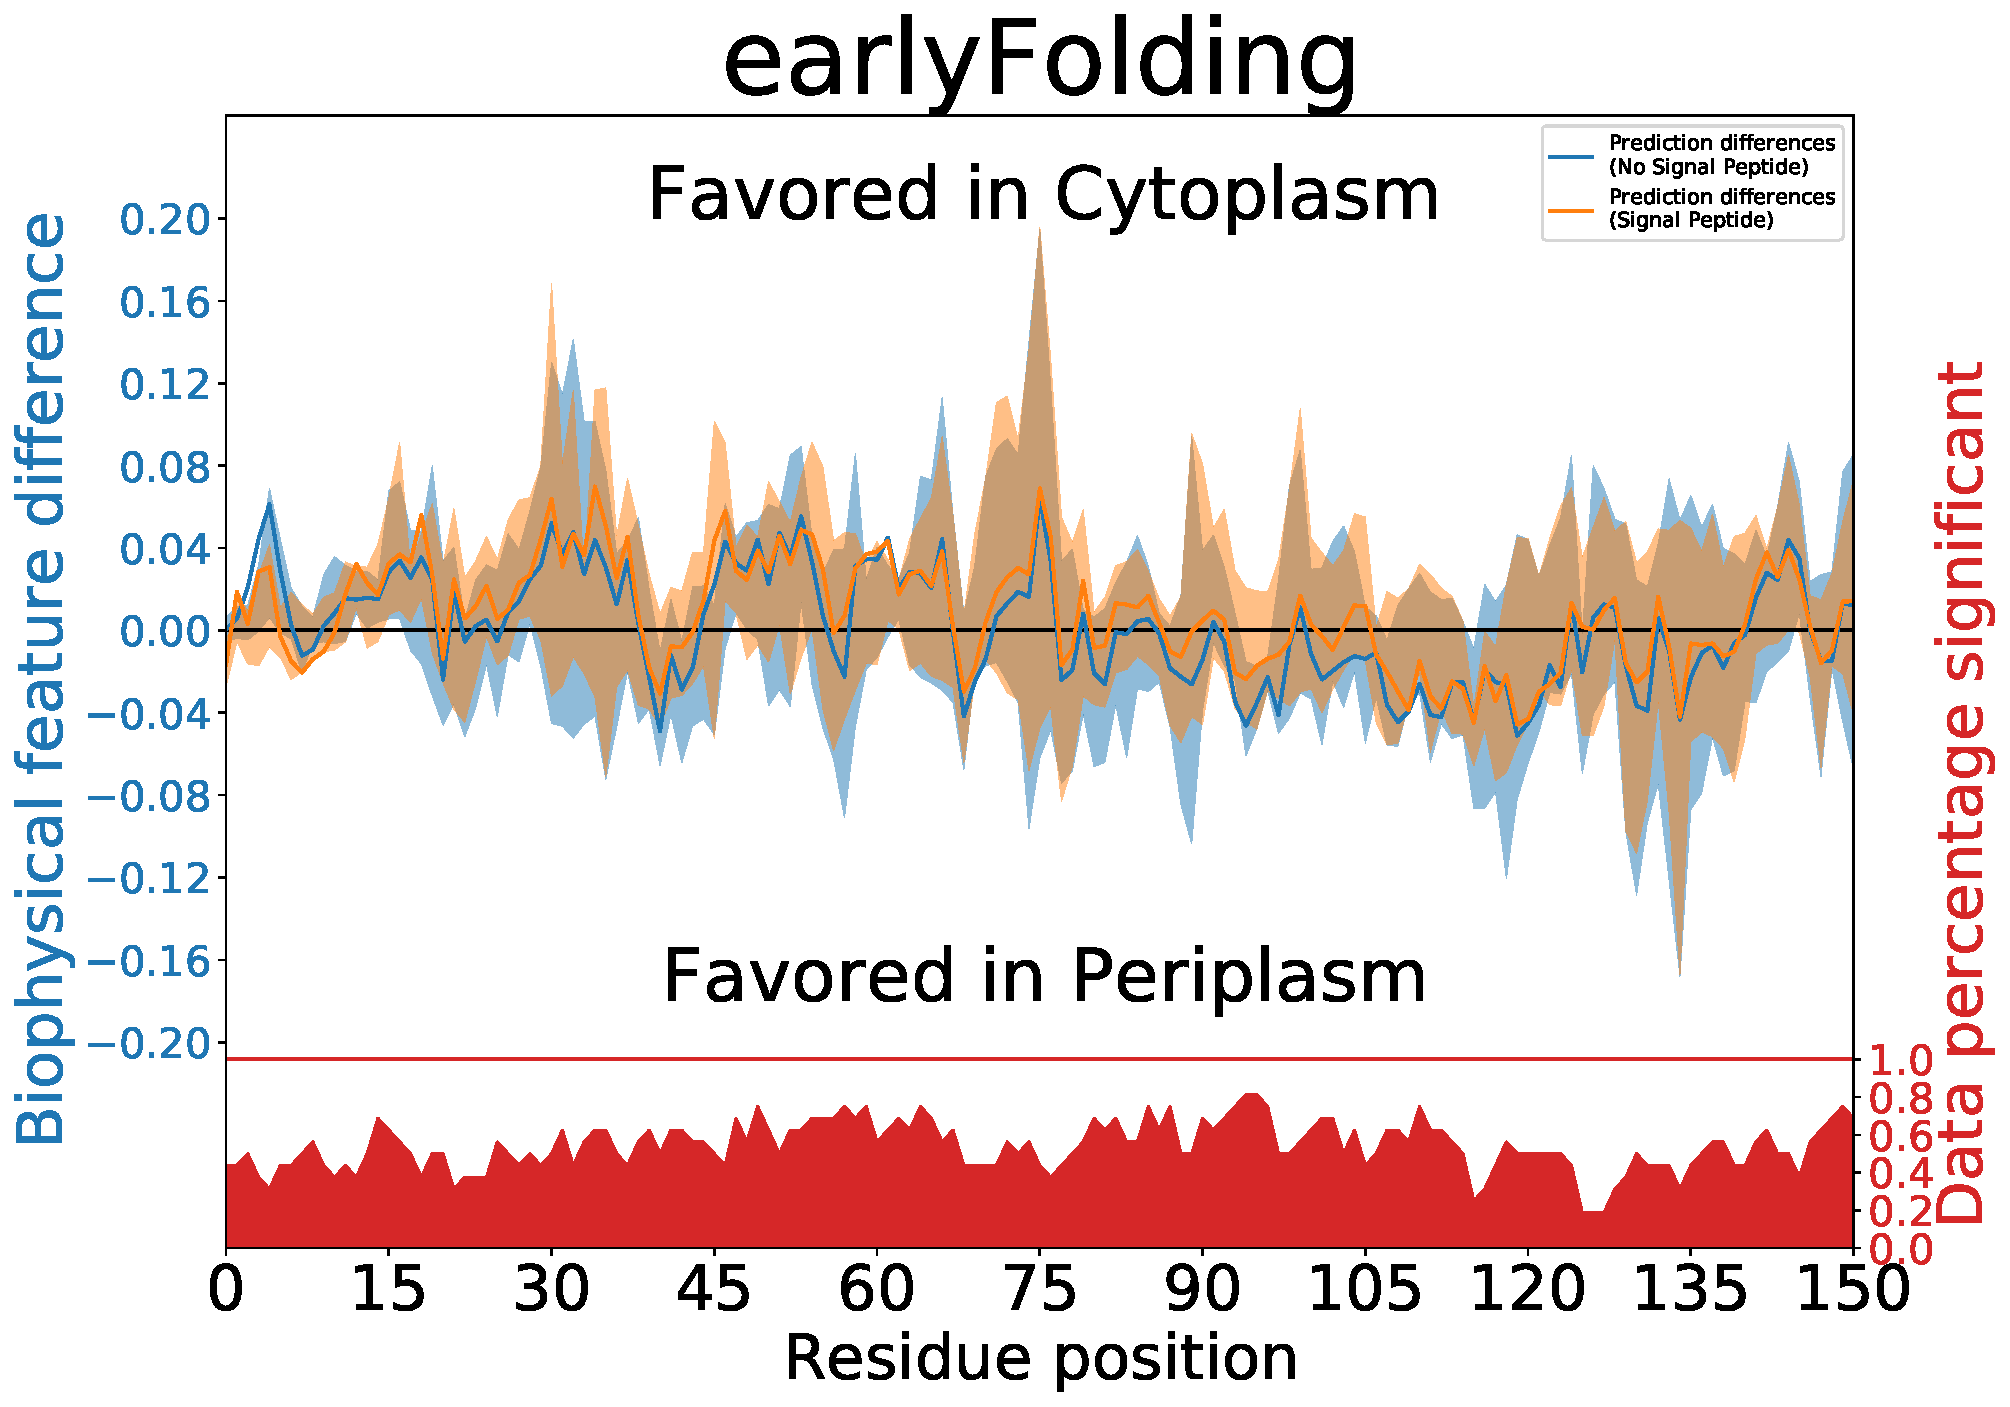
\includegraphics[width=\linewidth, height=0.43\textheight, keepaspectratio]
	{./results/twins/img/earlyFolding.pdf}
		\caption{}
		\label{fig:twin_earlyfolding}
	~\end{subfigure}
~\end{figure}


~\begin{figure}[h!]
	\ContinuedFloat
	~\begin{subfigure}[b]{\linewidth}
			\centering
			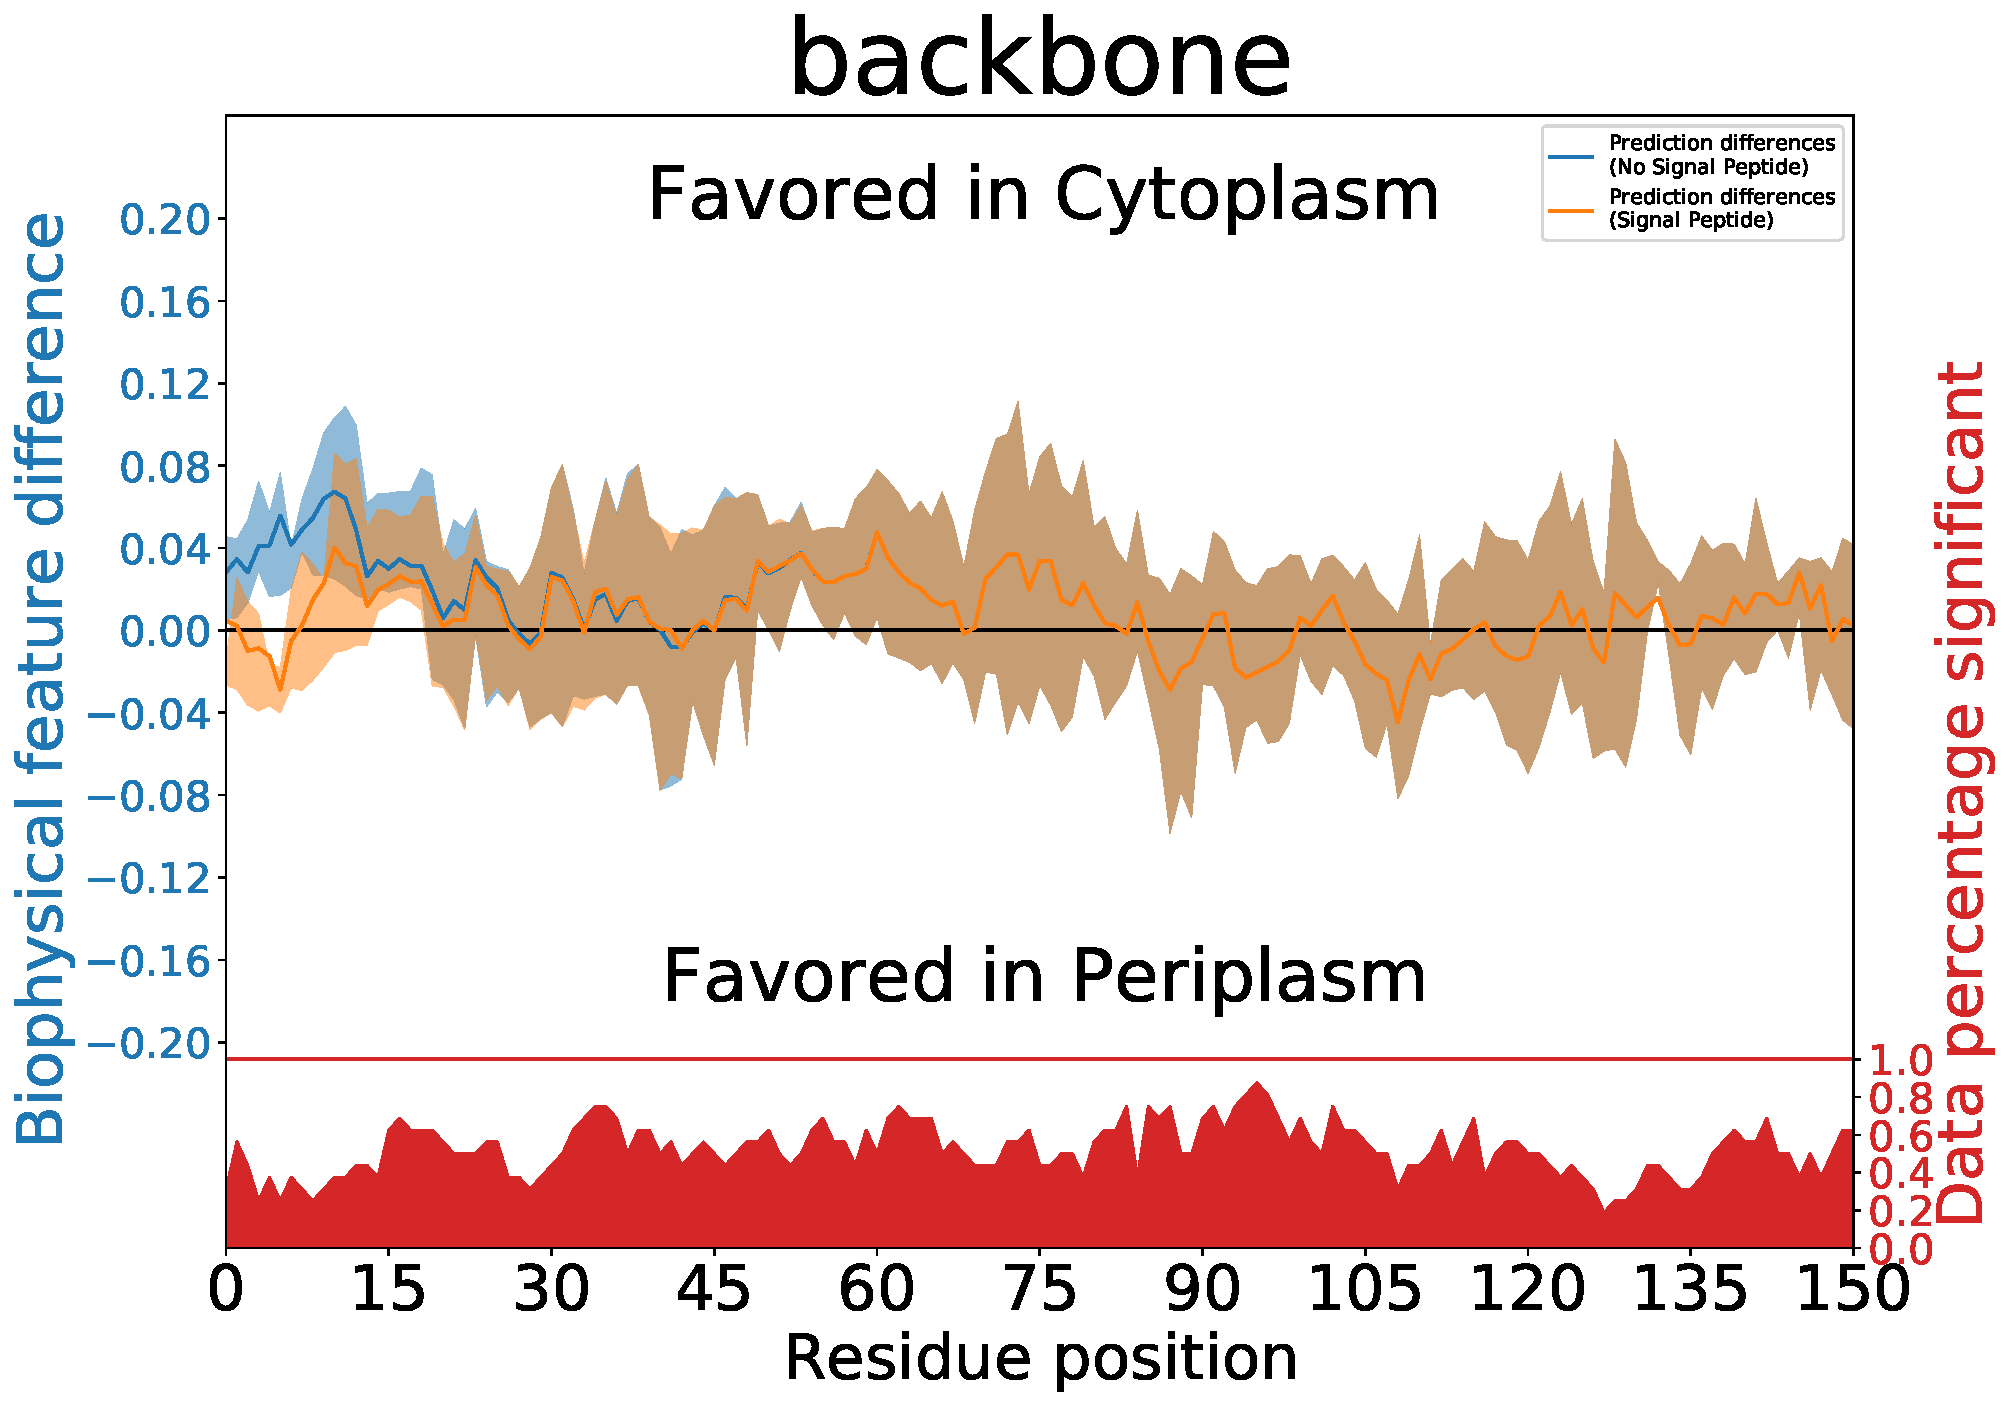
\includegraphics[width=\linewidth, height=0.34\textheight, keepaspectratio]
	{./results/twins/img/backbone.pdf}
		\caption{}
		\label{fig:twin_backbone}
	~\end{subfigure}
	\newline
	~\begin{subfigure}[b]{\linewidth}
			\centering
			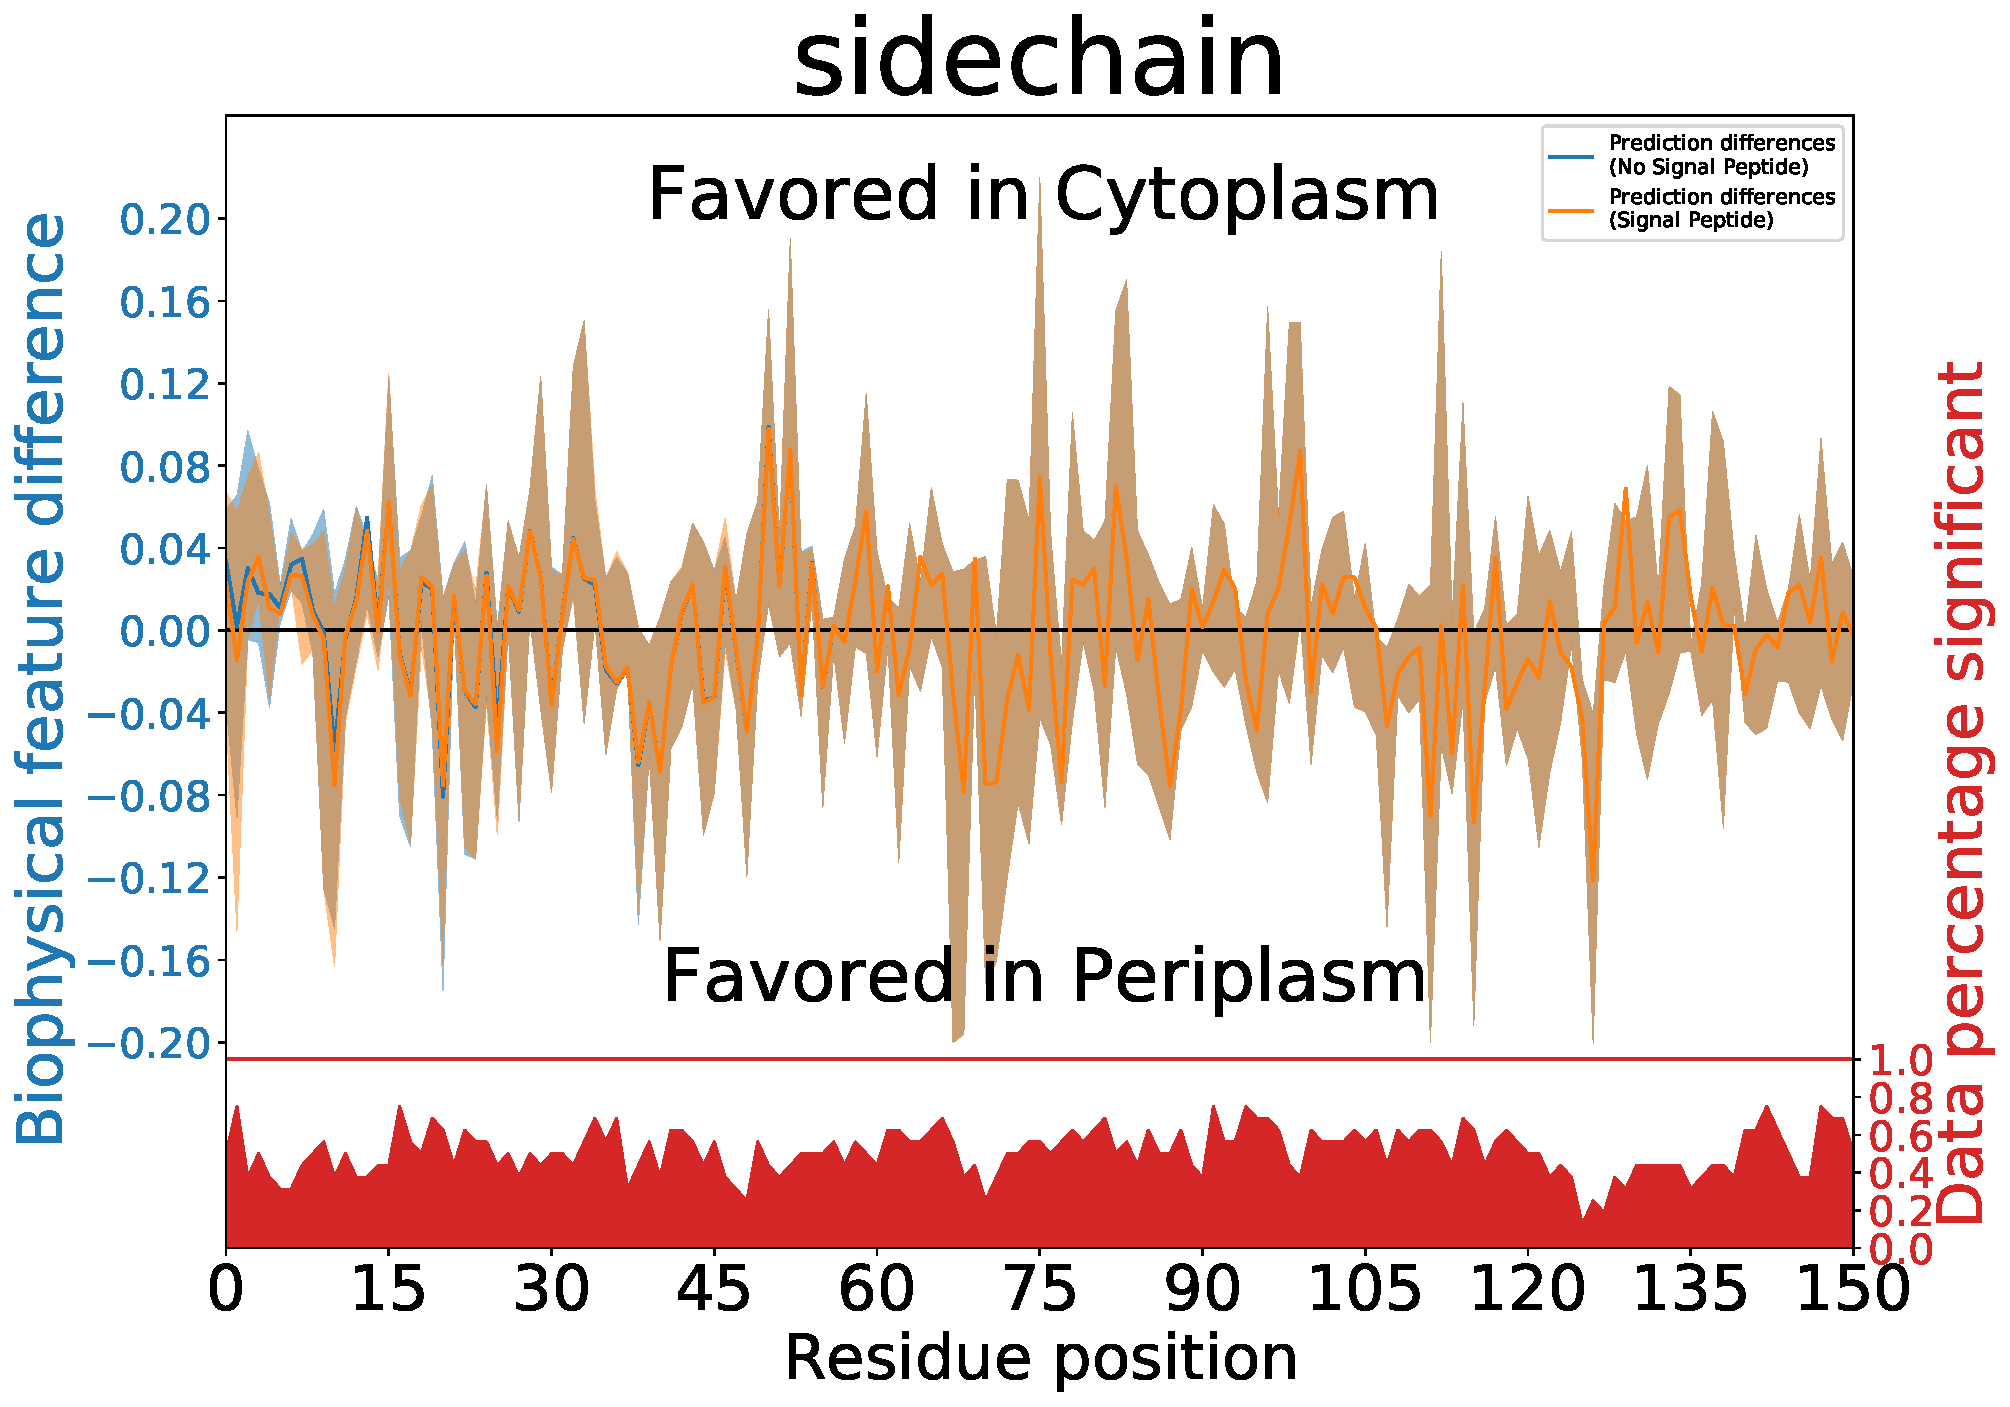
\includegraphics[width=\linewidth, height=0.34\textheight, keepaspectratio]
	{./results/twins/img/sidechain.pdf}
		\caption{}
		\label{fig:twin_sidechain}
	~\end{subfigure}
	\caption{
	\textbf{Difference in biophysical features between twins (first 150 residues)}
The difference of biophysical feature values is plotted in function of residue position.
The full line shows the median, the edge of the coloured area the quartiles,
75 percent of the observations fall within the coloured area.
Only significant differences were included (Wilcoxon-ranksum, P-value < 0.05).
To indicate how many observations of the 16 twins were included,
the red area at the bottom of the graphs gives a ratio between 0 and 1 for each position.
The Y-axis should be interpreted in the following way:
positive differences mean that cytoplasmic proteins tend to have a higher value for a certain property,
negative differences when the periplasmic proteins have a higher value.
Distinction is made between predictions with signal peptide (orange) and without signal peptide (blue).
Signal peptides themselves are not included in the graph.
}
~\end{figure}

	\subsection{Separation of cytoplasmic and periplasmic proteins in UniRep biophysical feature space}
		Before a machine learning based predictor can be trained to decode biophysical features from protein sequence.
A training set needs to be created either by performing the experiments,
or by gathering publicly available data.
UniProtKB has around 180 million protein sequences available,
but only 560,000 of those are reviewed, 
potentially containing the experiments with the biophysical features that a predictor needs to learn.
This covers only 0.3 percent of the sequence space, 
meaning that most of it remains largely unexplored.
However, the knowledge that a protein exist, is already important information.
The fact that evolution has come up with a specific combination of amino acids to fulfill some (unknown) function is already important information. 
The question remains how to incorporate this into the training data.

One way to partly alleviate this limitation is by considering a protein sequence with known function or biophysical properties and assuming that sequences with a certain percentage of sequence identity will have similar biophysical features and function.
This is in fact largely what the automated annotation system of UniProtKB is based on.
One way to subsequently incorporate such evolutionary information into the predictor would be by aligning the homologues sequences into a multiple sequence alignment and take amino acid variation into account.
While such methods cover a considerably larger portion of the sequence space, 
it only works if at least one homologue has been experimentally described, and more to have some confidence.
Regions in the sequence space without any experimental information are still neglected.

\cite{alley2019} tried to use the full potential of the sequence space by training a 
multiplicative long short-term memory recurrent neural network
(mLSTM RNN) with the task of next character prediction.
To get better at this task,
the neural networks changes the weights of its hidden neurons,
effectively discovering protein features in a unsupervised way.
Since only protein sequence information needs to be known,
all regions of proteins sequence space are included in the training.
When trained, a sequence can be used as input to the neural network,
and the hidden states extracted into a fixed length vector,
which forms a semantically rich representation of the protein.
The research group called this the UniRep representation.
Humans cannot interpret this representation directly,
but machine learning methods can used it to train a predictor, 
for example for biophysical features.
Even though experimental data is still necessary for that,
the UniRep representation makes it possible for these predictions to be more generalized,
as information from the whole protein sequence space is incorporated.


% 	\subsection{Signal peptide clustering }
	\subsection{Structural information available for twins}
	The analysis in of this master thesis was purely sequence based.
In a next step it would be interesting to include pdb structures.
Therefore, the UniProtKB mapping API was used to map available structures to twin proteins (Table. \ref{table:structures}).

\newpage
\begin{longtable}[]{@{}lll@{}}
\toprule
& ACC & PDB\tabularnewline
\midrule
\endhead
0 & A0A156C5X3 & {[}5Z66, 5Z6H{]}\tabularnewline
1 & P00805 & {[}1HO3, 1IHD, 1JAZ, 1JJA, 1NNS, \tabularnewline
	& & 3ECA, 4ECA, 5MQ5, 6EOK, 6NX6, \tabularnewline
	& &6NX7, 6NX8, 6NX9, 6NXA, 6NXB, \tabularnewline
	& &6PA2, 6PA3, 6PA4, 6PA5, 6PA6, \tabularnewline
	& & 6PA8, 6PA9, 6PAA, 6PAB, 6PAC{]}\tabularnewline
2 & P0A962 & {[}2HIM, 2P2D, 2P2N, 6NXC, 6NXD{]}\tabularnewline
3 & P0AFL3 & {[}1CLH, 1J2A, 1V9T, 1VAI{]}\tabularnewline
4 & P12994 & {[}1FJJ, 1VI3{]}\tabularnewline
5 & P13482 & {[}2JF4, 2JG0, 2JJB, 2WYN{]}\tabularnewline
6 & P21517 & {[}5BN7{]}\tabularnewline
7 & P23869 & {[}1LOP, 2NUL, 2RS4{]}\tabularnewline
8 & P45523 & {[}1Q6H, 1Q6I, 1Q6U, 4QCC{]}\tabularnewline
9 & P77368 & {[}1FUX{]}\tabularnewline
10 & P83223 & {[}1D4C, 1D4D, 1D4E{]}\tabularnewline
11 & Q72EC8 & {[}2XVX, 2XVY, 2XVZ{]}\tabularnewline
12 & Q9Z4P0 & {[}1QO8{]}\tabularnewline
\bottomrule
\caption{\textbf{PDB structures available for twins.}
	\textbf{ACC.} Accession code used by UniProtKB.
	\textbf{PDB.} Accession code used by PDB.
}
\label{table:structures}
\end{longtable}


\newpage

\section{Conclusions}
	% Rehearsal of main question
Examination of the difference in global biophysical features between cytoplasmic and periplasmic proteins in Gram-negative Bacteria seems to agree with the observations made by \cite{loos2019}.
Periplasmic proteins show an increased tendency towards the formation of coil and sheet structures,
but decreased propensity towards the formation of helical structures.
On average, periplasmic proteins display lower backbone and sidechain dynamics,
and a decreased tendency towards early folding.
This agrees with the hypothesis that periplasmic proteins have to delay the folding process to translocate to the periplasm.

% Main features observed (confirmation of other paper)
Region specific differences in biophysical features were examined by two complementary approaches.
The general approach including the periplasmic and cytoplasmic proteins of the class of Gammaproteobacteria.
In general, cytoplasmic proteins seem to display a region of increased flexibility and dynamics , and reduced propensity towards early folding near postion 10 to 20. 
In periplasmic proteins this region is extended by roughly 10 amino acids and has a slight shift towards the C-terminal end.
The first 10 amino acids however, 
display an increased tendency to early folding, 
an effect induced by the signal peptide.
Another interesting observation is that cytoplasmic proteins have an above average propensity to form a helix near position 25,
even while propensities to form a helix are averaged out over the large dataset in the rest of the protein.
In contrast, periplasmic proteins tend to have a decreased tendency towards helix formation starting from that same region until residue 70.
Periplasmic proteins have an increased tendency to form coil like structures and display increased backbone flexibility from position 20 to 70, 
except near position 33 where there is an increased tendency towards early folding and the formation of a sheet.

% local features observed by two complementary approaches
Similar differences were observed in the twin approach.
The effect of signal peptides on biophysical features near the N-terminal end was again observed,
most strongly in propensity towards helix formation and backbone dynamics.
As in previous approach, the region near position 33 is highlighted to display increased propensity towards early folding and decreased tendency to form helical structures in cytoplasmic proteins.
However, where in the general approach a tendency was seen to form sheet structures,
the twins showed by contrast an increased propensity to form helical structures.

% explanation
The reasons for these differences remain unclear.
Most likely, they are related to the delay of the folding process,
interactions with the translocation machinery,
or the formation of functional proteins in the periplasm.
It is possible that the high propensity towards early folding of the signal peptides,
and the increased propensity in the N-terminal region of the protein,
make very early folding foldons.
These foldons would than form interactions with other regions of the protein that do not occur in the fully folded structure,
thereby delaying the process.
The early folding region near position could possibly have a similar effect.
However, the position specificity seems to suggest that is forms some kind of interactions with translocation machinery.

% limitations
It should be noted that the tendencies described above don't need to be part of the same mechanism.
Also, there are very likely many biophysical differences that are position aspecific,
and can therefore not be elucidated by the analysis described above.
This research was purely based on sequential information and the predictions generated with these sequences.
However, a list of protein structures is provided as it was very straight forward to get these results with the UniProtKB pipeline that was designed for this master thesis. 
This list could be interesting to other research groups.

% UniRep prediction
Finally, the UniRep (\cite{alley2019}) representation was used to make classifiers that separates cytoplasmic and periplasmic proteins.
It showed that even without including signal peptides,
almost 95 percent of the proteins could be  correctly classified, 
which stresses the importance of the mature domain.
Though this was only an exploratory analysis, and a more rigorous approach should be performed to have u predictors.
The usage of UniRep vectors seems very promising.
Most importantly, they stress the fact there is a huge potential to use the undescribed protein sequences.
Including this information could improve the performance of predictors and make them applicable on a wider portion of the protein sequence space.

\newpage

\section*{Summary}
	% Part about UniProtKb
The amount of protein sequences in UniProtKB has been growing exponentially,
but experimental information of functionality or biophysical features is only available for about 0.3 percent of the protein sequence space.
% Relation between protein function and primary sequence
Local and distant interactions along the primary structure guide the folding process,
thereby determining structure , dynamics and function.
Essentially, all of the biophysical features are encoded within the amino acid sequence.
However, extracting those features has proven to be challenging and is still a topic of ongoing research.

% More specific about dynamics
Traditionally, protein function was thought to be a direct result of protein structure,
But in recent years it has become clear that structure provides only part of the picture.
Other biophysical features, such as the propensity toward dynamics, disorder, and early folding also seem to play a fundamental role for protein functionality.
A new generation of machine learning based predictors that only need a single protein sequence as input
are being developed at the Bio2Byte research lab at the Interuniversity Institute of Bioinformatics in Brussels.
Not only can these predictors predict biophysical features without relying on prior structural knowledge,
the predictions are also very fast,
making them scalable for computational high-throughput methods.

% What is unknown and what was researched
In this master thesis,
the biophysical features of cytoplasmic and periplasmic proteins were compared on an extensive Gram-negative Bacteria protein dataset.
Additionally, the effect of signal peptides on these features was examined.
This problem was approached from different directions.
A global approach showed that on average,
an increased tendency towards the formation coil and sheet structures,
but decreased propensity towards the formation of helical structures was observed in periplasmic proteins.
They also displayed lower backbone and sidechain dynamics,
and an decreased tendency towards early folding.
Two complementary positon specific approaches agreed on different features.
Signal peptides seem the promote the propensity towards helix formation and early folding in the N-terminal region of periplasmic proteins, 
but have an decreased propensity in the rest of the protein.
Additionally, a region near position 33 was observed with increased early folding propensity and decreased coil formation.
In a final approach, UniRep representations were utilized to make a predictor that can distinguish cytoplasmic and periplasmic proteins.


\newpage

\printbibliography
\newpage

\section*{Appendix}
		\subsubsection*{uniprotRetrieve.py}
			\inputpython{appendix/uniprotRetrieve.py}{1}{1000}
		\subsubsection*{uniprotMapping.py}
			\inputpython{appendix/uniprotMapping.py}{1}{1000}
		\subsubsection*{generateDatabases.py}
			\inputpython{appendix/generateDatabases.py}{1}{1000}
		\subsubsection*{runblast.py}
			\inputpython{appendix/runBlast.py}{1}{1000}
		\subsubsection*{runCDHIT.py}
			\inputpython{appendix/runCDHIT.py}{1}{1000}
		\subsubsection*{runCDHIT.py}
			\inputpython{appendix/runClustalOmega.py}{1}{1000}
		\subsubsection*{efoldminePredictionsMsa.py}
			\inputpython{appendix/efoldminePredictionsMsa.py}{1}{1000}
		\subsubsection*{clusterByOrganism.py}
			\inputpython{appendix/clusterByOrganism.py}{1}{1000}
\newpage

\end{document}
